\documentclass[journal]{IEEEtran}
\usepackage{iftex}
\ifPDFTeX
  \usepackage[T1]{fontenc}\usepackage[utf8]{inputenc}\usepackage{textcomp}
\else
  \usepackage{fontspec}
  \setmainfont{texgyretermes}[Extension=.otf,UprightFont=*-regular,BoldFont=*-bold,ItalicFont=*-italic,BoldItalicFont=*-bolditalic]
  \edef\termesid{\rmdefault}\DeclareFontFamilySubstitution{TU}{ptm}{\termesid}
\fi
\usepackage{amsmath,amssymb}
\usepackage{graphicx,longtable,booktabs,array,calc,cite,url}
\usepackage[hidelinks]{hyperref}
\providecommand{\tightlist}{\setlength{\itemsep}{0pt}\setlength{\parskip}{0pt}}
\makeatletter\newsavebox\pandoc@box
\newcommand*\pandocbounded[1]{\sbox\pandoc@box{#1}\ifdim\wd\pandoc@box>\linewidth\resizebox{\linewidth}{!}{\usebox{\pandoc@box}}\else\usebox{\pandoc@box}\fi}\makeatother
\newsavebox\mwbox\newcommand\maxwbox[2]{\sbox\mwbox{#2}\ifdim\wd\mwbox>#1\resizebox{#1}{!}{\usebox\mwbox}\else\usebox\mwbox\fi}
\setlength{\LTcapwidth}{\textwidth}\setlength{\tabcolsep}{4pt}
\begin{document}
\bstctlcite{IEEEexample:BSTcontrol}
\title{Toward a Foundation Model for NAION Risk Stratification in GLP-1 Receptor Agonist Users: Machine Learning, Graph Neural Networks and Synthetic Digital Twins Built from PubMed-Indexed Evidence}
\author{Kemar Earl Green, DO, FANA\textsuperscript{1,2}\thanks{Research prototype: uses only published aggregate data and computationally generated synthetic records (synthetic\_only twins; compliance reference Addendum 5, DT\#9); not validated for clinical, diagnostic, treatment-selection or regulatory use. This preprint has not been peer reviewed. \copyright\ 2026 NeuroAgent AI, Inc.; code, model weights and data are licensed for non-commercial research use only, with attribution.}\\[4pt] {\normalsize\itshape \textsuperscript{1}Johns Hopkins Data Science and AI Institute, Baltimore, MD, USA\\ \textsuperscript{2}NeuroAgent AI, Inc., Baltimore, MD, USA\\[2pt] \upshape\texttt{kemarearlgreen@neuroagentai.org}}}
\markboth{}{Green: GLP-1 receptor agonists and NAION --- ML on published evidence}
\maketitle
\begin{abstract}
\emph{Background:} Observational studies and pharmacovigilance reports
link glucagon-like peptide-1 receptor agonists (GLP-1RAs), particularly
semaglutide, to nonarteritic anterior ischemic optic neuropathy (NAION),
but no tool stratifies individual risk. Whether machine learning (ML) on
published evidence, with or without synthetic digital twins, can do so
is unknown. \emph{Methods:} We extracted data from 73 of 169 PubMed
publications and reconstructed count-weighted patient-level data from 11
non-overlapping cohorts (3,271,499 patients; 1,425 events). Logistic
regression, random forest, XGBoost, graph neural networks and ensembles
were trained on 10\% and tested on 90\%, across 10 disjoint 10\% folds,
across training fractions of 10\% to 90\%, and by leave-one-study-out
validation. Synthetic twins were added in a factorial grid. SHAP values,
permutation tests and Benjamini-Hochberg correction were used.
\emph{Results:} Within studies, GLP-1RA exposure was associated with
NAION (odds ratio 1.59 (95\% CI, 1.42 to 1.77)); semaglutide 1.73 (95\%
CI, 1.44 to 2.08); obesity indication 2.70 (95\% CI, 1.64 to 4.44).
XGBoost discriminated modestly (AUROC 0.656 \ensuremath{\pm} 0.011; observed/expected
1.00) but fell to 0.534 in unseen studies. At the top-10\% threshold,
PPV was 0.087\% against a prevalence of 0.044\%. Neither graph or
convolutional networks, ensembles nor added vascular-score features
outperformed PubMed-only XGBoost; synthetic digital twins mainly
regularized weaker learners, and the best hybrid XGBoost gained 0.0015
AUROC. Simulated addition of optic-disc imaging raised AUROC to about
0.82 to 0.84. \emph{Conclusions:} Published evidence supports a
reproducible exposure signal but only modest, setting-dependent risk
discrimination. The score suits research enrichment, not treatment
selection; patient-level prospective data are required.
\end{abstract}
\begin{IEEEkeywords}
Nonarteritic anterior ischemic optic neuropathy, GLP-1 receptor agonists, semaglutide, machine learning, synthetic data, digital twins, graph neural networks, risk prediction, explainable AI
\end{IEEEkeywords}
\section{Introduction}\label{introduction}

Nonarteritic anterior ischemic optic neuropathy (NAION) is the most
common acute optic nerve disease of adults older than 50 years
\cite{p9186104}. Population-based estimates of its annual incidence in
people aged 50 years or older range from 2.30 per 100,000 in Missouri
and Los Angeles County \cite{p8032479} to approximately 10 per 100,000
in Olmsted County, Minnesota, where incidence has remained stable over
four decades \cite{p9186104, p38358828}. The disorder presents as
abrupt, painless monocular vision loss with optic disc edema
\cite{p37987292}, and visual symptoms are frequently first noticed on
waking, as reported by 42\% of patients in the Ischemic Optic Neuropathy
Decompression Trial (IONDT) cohort \cite{p8906027}. About half of
affected eyes present with near-normal visual acuity, and visual acuity
and fields change mainly during the first 6 months \cite{p17698200}.
The fellow eye is affected in roughly 15--21\% of patients over several
years \cite{p12208242, p38358828}, with diabetes and worse first-eye
visual function predicting second-eye involvement
\cite{p12208242, p36502803}, whereas recurrence in the same eye is
uncommon \cite{p11704035}. Because the visual deficit is usually
permanent and bilateral disease is not rare, even small changes in
incidence carry meaningful population consequences.

The leading anatomic risk factor is a small, crowded optic disc with
little or no physiologic cup, the so-called disc at risk
\cite{p6514298, p3684223}. In the 729-participant Quark207 trial
cohort, a small fellow-eye cup-to-disc ratio was the most prevalent risk
factor across countries, races and sexes, whereas cardiovascular risk
factors were not typically more prevalent than in the general population
\cite{p38211825}. Optic disc drusen are found in most younger patients
with NAION and may act as an independent risk factor
\cite{p32298654, p31972711}. Systemic associations include
hypertension, diabetes, hyperlipidemia, coronary heart disease, male sex
and obstructive sleep apnea, as summarized in a meta-analysis of 49
studies \cite{p34671609} and in cohort and case-control studies
\cite{p7977604, p9366670, p27659545}; sleep apnea carries one of the
largest relative risks in pooled analyses \cite{p26443989, p34671609}.
Nocturnal arterial hypotension has been proposed as a final insult that
lowers optic nerve head perfusion below a critical level in susceptible
patients \cite{p8172267} and has been associated with same-eye
recurrence \cite{p11704035}. Other reported precipitants include
cataract surgery, after which relative risk rises within the first year
although absolute risk remains low \cite{p36166807, p32818451};
perioperative blood loss, hypotension and anemia \cite{p18358851}; and
hemodialysis-related hypotension and anemia \cite{p11730278}. Drug
associations remain debated: pooled observational data did not show a
significant association with phosphodiesterase-5 inhibitors
\cite{p31559705}, although a case-crossover study reported a 2-fold
increase in risk \cite{p26720519}; a causal link with amiodarone has
never been firmly established \cite{p16148635}; and interferon alfa is
classed as a ``possible'' association \cite{p20630599}. Evidence on
smoking \cite{p17398323} and thrombophilia is inconsistent, with one
case-control study finding no association with thrombophilic markers
\cite{p10201595}, while a managed-care cohort \cite{p27659545} and
small case-control data \cite{p15834600} reported positive
associations. The optic nerve head is supplied by the short posterior
ciliary arteries, and NAION is attributed to infarction of the laminar
and retrolaminar optic nerve head \cite{p19596112}. Proposed
contributors include nocturnal hypotension, impaired autoregulation,
vasculopathic occlusion and venous insufficiency \cite{p19596112}.
Clinicopathologic and blood-flow data point to vasculopathy within or
distal to the paraoptic branches, with diabetes the most consistently
identified vasculopathic risk factor \cite{p12782932}. A widely cited
model holds that ischemic axonal swelling within a crowded disc produces
a compartment syndrome \cite{p19596112}; three-dimensional
reconstruction of a human infarct did not correspond to a single
vascular territory, consistent with this view \cite{p14522783}. Hayreh
argued that vascular insufficiency of the optic nerve head underlies
AION while noting conflicting interpretations of its blood supply and of
measurement methods \cite{p11470451}. Rodent and primate photoembolic
models reproduce disc edema followed by retinal ganglion cell loss
\cite{p14507856, p18326695}, but much of the pathophysiology remains
unknown \cite{p26959135}.

No treatment for NAION is proven \cite{p25763979, p35270411}. The
IONDT, a randomized trial of optic nerve decompression surgery, was
stopped early; surgery was not effective and may have been harmful
\cite{p7844872}, and 24-month follow-up confirmed no benefit
\cite{p10865316}. Spontaneous improvement among patients in the careful
follow-up group was more common than previously reported
\cite{p7844872}. A large nonrandomized cohort reported better acuity
outcomes with systemic corticosteroids \cite{p18404273}, but a small
randomized trial \cite{p29705054} and meta-analyses
\cite{p31725628, p35270411} did not show significant visual acuity
benefit. A 725-participant sham-controlled trial of intravitreal
QPI-1007 did not meet its primary endpoint \cite{p40816607}, and
evidence for levodopa comes from small or nonrandomized studies
\cite{p8554083, p10711891}. Antiplatelet evidence is limited to
observational data for fellow-eye protection. Retrospective studies
reported lower second-eye NAION with aspirin
\cite{p9427177, p10624433}, but a larger retrospective cohort found
possible short-term and little or no long-term benefit \cite{p9186127},
and aspirin use was not associated with fellow-eye NAION in the
prospectively followed IONDT cohort \cite{p12208242}. No randomized
evidence was identified for aspirin in any risk-defined subgroup,
including drug-associated NAION; this gap is relevant to whether
antiplatelet therapy could be targeted at high-risk patients.

GLP-1 is an intestinal L-cell hormone that augments insulin and
suppresses glucagon secretion, slows gastrointestinal motility and
reduces food intake, and is inactivated within minutes by dipeptidyl
peptidase IV \cite{p17928588, p29617641, p22945360}. GLP-1RAs range
from short-acting agents (exenatide twice daily, lixisenatide) to
once-daily liraglutide and once-weekly exenatide, dulaglutide and
semaglutide, and oral semaglutide is also available
\cite{p22945360, p33068776}. Semaglutide has a half-life of
approximately 1 week \cite{p27633186}, and tirzepatide is a dual GIP
and GLP-1 receptor agonist \cite{p35658024}. In placebo-controlled
trials, semaglutide 2.4 mg reduced body weight by a mean 14.9\% at 68
weeks \cite{p33567185}, and tirzepatide reduced it by 15.0--20.9\% at
72 weeks \cite{p35658024}. Tirzepatide lowered HbA1c by more than
semaglutide 1 mg in type 2 diabetes \cite{p34170647}. Cardiovascular
outcome trials showed reductions in major adverse cardiovascular events
with liraglutide, semaglutide and dulaglutide
\cite{p27295427, p27633186, p31189511, p31422062}, including in people
with obesity without diabetes \cite{p37952131}, and semaglutide reduced
kidney outcomes in chronic kidney disease \cite{p38785209}. Across
trials, GLP-1RAs modestly lower systolic blood pressure and slightly
raise heart rate \cite{p26358202}. Ocular and neural findings are
directly relevant to NAION. In SUSTAIN-6, semaglutide increased diabetic
retinopathy complications (hazard ratio 1.76) \cite{p27633186}, an
effect attributed mainly to the magnitude and speed of early HbA1c
reduction \cite{p29178519}. GLP-1 receptor expression in the normal
human eye is low and confined to a small fraction of ganglion-cell-layer
neurons \cite{p29707863}. GLP-1 receptor agonism lowered intracranial
pressure in a rodent hydrocephalus model \cite{p28835515} and in a
randomized trial of exenatide in idiopathic intracranial hypertension
\cite{p36907221}, although central receptor activation increased
cerebrospinal fluid secretion and intracranial pressure in another rat
study \cite{p40275284}.

After a neuro-ophthalmology cohort reported higher NAION risk among
patients prescribed semaglutide \cite{p38958939, p40055951}, a
nationwide Danish cohort \cite{p39696569}, a Danish nested case-control
study \cite{p42126975}, a US veterans target trial emulation
\cite{p41678180} and US electronic health record cohorts
\cite{p40146102, p40788646} reported hazard ratios of about 1.8--2.4.
In contrast, a multinational cohort found no significant association
\cite{p39491755}, and a 14-database network found mostly null
active-comparator estimates with a modest self-controlled signal
\cite{p39976940}. Meta-analyses range from a significant pooled risk
\cite{p42060879, p40810985} to signals confined to observational
diabetes studies \cite{p41475544} or no consistent increase with
low-certainty evidence \cite{p41692115}. Absolute risks are low
\cite{p41678180, p42132708}. The European Medicines Agency classifies
NAION as a very rare adverse effect of semaglutide \cite{p41857480},
and joint neuro-ophthalmology/ophthalmology and European
multidisciplinary consensus statements recommend shared decision-making
rather than class-wide restriction \cite{p42132708, p41058255}.
Proposed mechanisms remain hypotheses. They include rapid glycemic
lowering analogous to early worsening of retinopathy
\cite{p40055951, p41857480}, blood-pressure and nocturnal-pressure
lowering \cite{p41857480}, volume depletion from gastrointestinal
effects or rapid weight loss \cite{p41678180, p42773534}, and impaired
optic nerve head autoregulation \cite{p41678180}. Other proposals are
intracranial-pressure-mediated changes in retinal perfusion
\cite{p42335513, p42866022}, a ``two-hit'' model combining anatomic
susceptibility with hypohydration \cite{p42547311}, and
exposure-dependent pharmacokinetic thresholds favoring high-exposure
subcutaneous semaglutide \cite{p42770962}. Several of these proposals
are speculative or mutually inconsistent; the systemic vascular effects
of GLP-1RAs would be expected to reduce ischemic risk \cite{p42866022},
and blood pressure, dehydration and autonomic effects are described as
theoretical \cite{p42890826}. Crowded discs appear equally prevalent in
exposed and unexposed NAION \cite{p42556433}, and reviewers have called
for identifying which patient characteristics (disc anatomy,
blood-pressure change, weight loss, glycemic improvement) mark higher
risk \cite{p41022666}.

This evidence leaves several questions open: whether the signal is
causal, whether it differs by agent, dose, indication and duration
\cite{p42126975, p42770962}, and which patients are susceptible. The
aim of this study was to assess whether machine learning applied to
published evidence can stratify NAION risk among GLP-1RA users and which
features matter.

Beyond conventional supervised learning, we examined whether graph
neural networks that share information across similar patient profiles,
ensembles, convolutional networks and synthetic digital twins improve on
simpler models; whether a model of background NAION risk learned without
any GLP-1RA exposure transports to GLP-1RA users; and whether
fine-tuning such a model with real, synthetic or hybrid GLP-1RA data
improves risk stratification. Every comparison was tested statistically
with correction for multiple testing.

\section{Methods}\label{methods}

\subsection{Data sources and
extraction}\label{data-sources-and-extraction}

We searched PubMed for GLP-1RA or GIP/GLP-1RA terms combined with optic
neuropathy terms and retrieved 169 records, 60 with open-access full
text. Three extraction agents worked in parallel under a fixed schema:
patient-level rows from case reports, arm-level counts and effect
estimates from observational studies, and signal statistics and pooled
estimates from pharmacovigilance studies, pooled trials and
meta-analyses. Every value carries its PMID, an evidence level (full
text, abstract or publisher page) and a supporting quotation; unreported
values were left missing. One retracted article was excluded
\cite{p41144820, p42468029}.

\subsection{Reconstruction of patient-level
data}\label{reconstruction-of-patient-level-data}

For each of 11 cohorts with event counts in both arms we selected one
primary, non-overlapping contrast (Table~\ref{tbl:cohorts}); overlapping
Danish registry analyses and a case-control study were excluded from
reconstruction. Each arm became two rows (events, non-events) weighted
by their counts, carrying arm-level therapy and exposure and study-level
indication, region, data source, outcome definition, follow-up, mean age
and percentage female (study medians imputed with missingness
indicators). Because splitting patients uniformly at random is
equivalent to binomial or multinomial thinning of these counts, every
split below operates on individual patients without enumerating millions
of rows.

\subsection{Models and validation}\label{models-and-validation}

We trained L2-regularized logistic regression, random forest and XGBoost
\cite{chen2016} with count weights. Validation used (i) a single 10\%
training / 90\% test split; (ii) ten disjoint folds, each training on a
different random 10\% of patients and testing on the remaining 90\%;
(iii) training fractions from 10\% to 90\% in 10-point steps with 10
repeats each; and (iv) leave-one-study-out validation. We report AUROC,
PR-AUC, Brier score, calibration slope and observed-to-expected (O/E)
ratio, and sensitivity, specificity, accuracy, PPV and NPV at three
thresholds fixed on training data (Youden-optimal, top 10\%, top 20\% of
predicted risk), with net benefit \cite{vickers2006}.

\subsection{Graph neural networks}\label{graph-neural-networks}

Each distinct covariate pattern became a node; edges joined each node to
its k nearest neighbours in standardized feature space and linked the
exposed and comparator arms of the same study. A GraphSAGE network
\cite{hamilton2017} was trained with a count-weighted binomial loss on
training counts only. We varied depth (1 to 6 layers), neighbourhood
size (5, 10, 20), edge weighting (uniform or Gaussian kernels) and the
weight of same-study links, and compared learned edge weights through
graph attention \cite{velickovic2018}; configurations were selected on
folds 0 to 4 and confirmed on untouched folds 5 to 9. Attributions used
integrated gradients \cite{sundararajan2017}.

\subsection{Synthetic digital twins}\label{synthetic-digital-twins}

Twins were generated in a factorial grid \cite{montgomery2017} with
local refinement \cite{bergstra2012}: three generators (independent
marginals; Gaussian copula preserving feature correlations
\cite{patki2016}; a structural model on SHAP-stable features) and their
combinations, three prior sources (fitted to the real training split,
published external priors only, or a blend), six volumes (1 to 100 times
the real training size) and synthetic shares of 10\% to 100\%, crossed
with real training fractions of 0\% to 90\%, four models and 10 repeats.
Twins were never used for testing, and generators never saw test data.
Local refinement around the best cell continued while AUROC improved by
at least 0.005.

\subsection{Ensembles}\label{ensembles}

All combinations of two or more of logistic regression, random forest,
XGBoost and the GNN were combined by averaging, by weights from inner
cross-validation, and by stacking with a logistic meta-learner fitted on
inner out-of-fold predictions, and a cross-family ensemble averaged the
best PubMed-only, hybrid and synthetic-only models.

\subsection{Statistical analysis}\label{statistical-analysis}

Within-study effects were estimated with count-weighted logistic
regression with study fixed effects; marginal associations used
cluster-robust standard errors by study. SHAP values
\cite{lundberg2017} were tested against null distributions from 500
refits with events reallocated at random across arms, globally and
within studies. Published ratio estimates were pooled with
DerSimonian-Laird random effects \cite{dersimonian1986}. AUROC was
tested against 0.5 with the Hanley-McNeil method \cite{hanley1982};
models were compared with the Nadeau-Bengio corrected resampled t-test
\cite{nadeau2003} on paired folds and with exact McNemar tests;
sensitivity, specificity, PPV, NPV and accuracy were tested against
chance with exact binomial tests. P values within each family were
adjusted with the Benjamini-Hochberg procedure \cite{benjamini1995}.
Reporting follows TRIPOD+AI \cite{collins2024}.

\subsection{Detailed derivation of every
dataset}\label{detailed-derivation-of-every-dataset}

\textbf{Search corpus.} A single PubMed query combined drug terms
(semaglutide, tirzepatide, liraglutide, dulaglutide, exenatide, GLP-1,
glucagon-like peptide) with outcome terms (NAION, ischemic/ischaemic
optic neuropathy, optic neuropathy). Metadata, abstracts and PubMed
Central open-access full texts, including embedded tables, were
retrieved programmatically; publication types were recorded.

\textbf{Extraction datasets.} Four structured datasets were produced by
three independent extraction agents working from the same rules: (1) a
case-level table with one row per published patient (age, sex, drug,
formulation, dose, recent escalation, time to onset, indication,
comorbidities, disc morphology, drusen, dehydration, laterality, visual
acuity converted to logMAR, imaging available, treatment and recovery);
(2) a cohort-level table with one row per study, contrast and subgroup
(design, data source, population, exposure, comparator, arm sizes and
events, person-years, effect measure with CI, adjustment, follow-up and
population characteristics); (3) a pharmacovigilance table (database,
drug, formulation, subgroup, case counts, ROR, PRR, IC025, EBGM); and
(4) a pooled-trial and meta-analysis table (pooled estimates by subgroup
and risk factors named by consensus statements). Values not reported
were left missing; every row carries the PMID, evidence level and a
supporting quotation of at most 200 characters, and possible duplicate
cohorts were flagged.

\textbf{Reconstructed patient-level dataset (pseudo-IPD).} From the
cohort table we kept contrasts with event counts in both arms and
selected one primary, non-overlapping contrast per study, preferring
crude full-cohort counts and excluding overlapping national-registry
analyses and a case-control design. Each arm produced an event row and a
non-event row weighted by their counts. Arm-level variables were
exposure and therapy; study-level variables were indication, region,
data source, outcome definition, follow-up, mean age and percentage
female, with medians imputed and missingness flagged. Because uniform
random sampling of patients is equivalent to binomial (single split) or
multinomial (k-way partition) thinning of counts, every split is an
exact patient-level split.

\textbf{Non-GLP and GLP sub-datasets.} For transfer experiments the
reconstructed data were divided into comparator-arm patients (no
GLP-1RA) and exposed-arm patients. Background-risk models used only
features defined in both populations (exposure and therapy excluded).

\textbf{Synthetic datasets (digital twins \cite{kamelboulos2021}).}
Three generators produced twin profiles: a marginal generator sampled
each feature independently from training marginals with risk equal to
the therapy-stratum rate; a Gaussian-copula generator \cite{patki2016}
sampled joint covariate patterns with copula jitter on numeric features
and drew each twin's risk from the Beta posterior of its source pattern;
a structural generator used the copula generator's features with risk
from a logistic model restricted to SHAP-stable features. Generators
were fitted to the real training split only (source = real), to
published priors only (source = prior: a non-user baseline of about 1.35
per 10,000 person-years derived from a pooled incidence of 85 per
100,000 GLP-1RA users and a pooled ratio of 2.52 \cite{p42060879}, with
drug-specific ratios of 1.93 and 1.70 \cite{p42612051, p41498755}), or
to a 50/50 blend. Twin counts were distributed over a bank of 5,000
profiles by multinomial sampling and outcomes drawn binomially.

\textbf{Released datasets.} The search records, the four extraction
tables, the reconstructed counts, an exact 1\% patient-level expansion,
the Introduction evidence table and eight synthetic sets of 200,000
twins each (three generators \ensuremath{\times} two prior sources, plus non-GLP and GLP
populations) are released with a data dictionary and checksums.

\subsection{Detailed description of every
experiment}\label{detailed-description-of-every-experiment}

\textbf{Stage 1 --- PubMed-only supervised learning.} Logistic
regression (weights rescaled to the number of events so that the L2
penalty is meaningful), random forest and XGBoost were evaluated with a
10\%/90\% split, ten disjoint 10\% training folds and
leave-one-study-out validation; SHAP stability was summarized across
folds. \textbf{Stage 1b} clustered case-report patients (k-means,
Gaussian mixture, Ward; bootstrap co-assignment) and fitted a
random-forest meta-regression of published log ratios with grouped
cross-validation. \textbf{Stage 1c} repeated Stage 1 at training
fractions of 10\% to 90\% (10 repeats each) and measured SHAP-rank
agreement with Kendall's W.

\textbf{Stage 2 --- synthetic-data grid with local refinement.} XGBoost
was trained on mixtures defined by three generators, six volumes (1, 3,
6, 9, 27 and 100 times the real training size) and synthetic shares of
10\% to 100\%, crossed with real held-out fractions of 10\% to 100\% and
three seeds (5,310 fits). The training set of size V\ensuremath{\times}R contained
(1\ensuremath{-}s)\ensuremath{\times}V\ensuremath{\times}R real patients (sampled without replacement when available,
otherwise bootstrapped) and s\ensuremath{\times}V\ensuremath{\times}R twins. The grid was refined around the
best cell with halving steps while AUROC improved by \ensuremath{\geq}0.005 (maximum
depth 3).

\textbf{Stage 3 --- full factorial.} Four models (logistic regression,
random forest, XGBoost and their mean) trained on identical data per
cell; real training fractions 0\% to 90\%; seven generator sets (every
non-empty combination of the marginal, copula and structural
generators); three prior sources; six volumes; ten shares; ten repeats.
Differences from PubMed-only training on the same split were tested per
configuration (one-sided paired t) with Benjamini-Hochberg correction;
robust configurations were ranked across all training fractions under a
calibration constraint (\textbar O/E\ensuremath{-}1\textbar\textless0.10, slope 0.9
to 1.1).

\textbf{Stage 4 --- ensembles.} Eleven member subsets of logistic
regression, random forest, XGBoost and the GNN, three combiners (mean,
inner-CV AUROC weights, logistic stacking on inner out-of-fold logits)
and a cross-family ensemble, under the same split paradigms.

\textbf{Stage 5 --- inference.} Count-weighted logistic models (marginal
with cluster-robust errors; within-study with study fixed effects,
including exposure by drug, indication, comparator and study-level age,
sex and follow-up); SHAP permutation tests (500 refits, global and
within-study nulls); random-effects meta-analysis with subgroup tests;
demographic contrasts (exact binomial, Wilcoxon, ratio-of-ratios z
tests); and threshold metrics with tests against chance, McNemar and
corrected resampled t comparisons, and net benefit.

\textbf{Stage 6 --- graph neural networks.} GraphSAGE on a pattern graph
(k-nearest neighbours plus same-study links), with integrated-gradient
attributions, under all split paradigms; \textbf{Stage 6c} tuned depth
(1 to 6), k, edge weighting and same-study weight (360 configurations)
and learned attention weights (graph attention network, depths 1 to 6),
selecting on folds 0 to 4, confirming on folds 5 to 9 and testing the
top configurations by leave-one-study-out validation.

\textbf{Stage 7 --- background-risk model with external validation in
GLP-1RA users.} Models trained only on non-GLP patients (internal splits
as above) were applied to all GLP-1RA-exposed patients to discriminate
NAION from no NAION; observed-to-expected ratios with exact Poisson
intervals quantify how much a background model under-predicts GLP-1RA
users. A GLP-aware model trained on both arms served as reference.

\textbf{Stage 8 --- fine-tuning.} Within each of five repeats, non-GLP
patients were split 80/20 (pretraining pool, forgetting test) and GLP
patients 50/10/40 (fine-tuning pool, validation, test). Pretraining
sources (none, real, synthetic, hybrid) were crossed with fine-tuning
sources (real, synthetic, hybrid) and GLP fractions (0\%, 5\%, 10\%,
25\%, 50\%). Update methods were recalibration in the large, logistic
recalibration, continued XGBoost boosting from the pretrained margin
(rounds selected on validation), GNN joint training with GLP
up-weighting (selected on validation), pooled refitting and GLP-only
training. Three additional split schemes tested transport in each
direction and the standard mixed split.

\textbf{Stage 10 --- incidence, rare-event and anomaly models.}
Incidence rates per 100,000 person-years used reported person-years
where available and otherwise N \ensuremath{\times} follow-up; rates were stratified by
drug, indication, comparator, region, data source, study age band,
percentage female and follow-up, with exact conditional confidence
intervals for incidence rate ratios, Mantel-Haenszel ratios stratified
by study and Poisson models with study fixed effects,
exposure-by-stratum terms and a log person-time offset (Wald tests of
heterogeneity). Rare-event learners were a Poisson rate model with
offset, class-weighted XGBoost with prior correction, King-Zeng
corrected logistic regression, a focal-loss network and
incidence-anchored XGBoost recalibrated to observed incidence within
exposure-by-age strata. Anomaly detectors (Isolation Forest, one-class
SVM, Local Outlier Factor and an autoencoder) were trained on non-event
patients of the training split only.

\textbf{Stage 11 --- detection within GLP-1RA users and within
non-users.} Every model (logistic regression, random forest, XGBoost,
GNN, 1D-CNN, mean ensemble, Poisson rate model, Isolation Forest and
autoencoder) was trained on mixed data in each of the ten folds and
evaluated separately within the exposed and unexposed parts of the test
set (AUROC, PR-AUC, O/E, calibration slope and threshold metrics at the
training top-10\% threshold); group differences were tested with
corrected paired t tests and Benjamini-Hochberg correction.

\textbf{Stage 12 --- validated vascular score and a proposed
NAION-adapted score.} The ABCD2 score and its newest extension ABCD3-I
were derived where possible (age 60 years or older as the expected share
from study mean age with an assumed SD of 12 years; blood pressure from
hypertension prevalence; diabetes from the study population) and used
only as features. A points score was fitted to the data and, separately,
built from published patient-level ratios and our within-study GLP-1RA
estimates, with points equal to log ratio divided by log 1.28
(hypertension = 1 point), recalibrated on training data and validated
with the same splits. \textbf{Stage 12b} repeated every experiment with
and without the ABCD features using identical splits and seeds, so that
all differences are paired.

\textbf{Stage 14 --- feature combinations and the compounding
hypothesis.} Because a calculator should accept whatever inputs are
available, models were trained on every non-empty combination of nine
feature groups (exposure, drug, indication, age, sex, duration,
hypertension, diabetes and setting; 511 combinations) with logistic
regression, random forest and XGBoost on all ten folds and with the GNN,
1D-CNN and mean ensemble on three folds. Exact Shapley values and
pairwise Shapley interaction indices of AUROC quantified each group's
contribution across all coalitions; the hypothesis that individually
negligible groups contribute in combination was tested on fold-level
values with corrected t tests and Benjamini-Hochberg correction. A
single XGBoost trained with random feature-group dropout was compared
with a bank of dedicated sub-models for each input pattern.

\textbf{Stage 9 --- convolutional networks and multimodal feasibility.}
A one-dimensional CNN treated the encoded feature vector as a sequence
(two convolution layers, global max pooling and a skip connection) under
the same paradigms. A two- and three-dimensional imaging pipeline
(fundus and OCT volume encoders, late fusion with tabular features and
Grad-CAM) was implemented and verified on random tensors, but could not
be trained because no analysable images exist in the published corpus.

\textbf{Stage 15 --- compute, energy and token use.} Energy was
estimated with the Green Algorithms method (runtime \ensuremath{\times} {[}cores \ensuremath{\times}
per-core power + memory \ensuremath{\times} 0.3725 W/GB{]} \ensuremath{\times} PUE) for an Apple M3 Pro
laptop (PUE 1.0, package power 25 to 45 W), with run times taken from
each stage's log where available, and converted to CO2e at 0.10 to 0.70
(central 0.367) kgCO2e/kWh. Inference time was measured per 1,000
predictions. Tokens consumed by the AI assistant were recorded where
metered.

\textbf{Stage 16 --- what-if: multimodal ocular imaging.} For each
reconstructed patient, imaging features were drawn conditional on the
observed outcome (P{[}feature \textbar{} NAION{]} \ensuremath{\propto} prior \ensuremath{\times} odds ratio;
P{[}feature \textbar{} no NAION{]} = prior), independently across
features: cup-to-disc ratio categories with the published control
distribution and odds ratios (fundus photography with 25\% and OCT with
5\% adjacent-category misclassification), and hypothetical optic disc
drusen (prevalence 2\%, odds ratio 2 to 8), OCT angiography
hypoperfusion (20\%, 1.5 to 3) and serial on-treatment imaging change
(5\%, 2 to 10), with sleep apnoea (27\%, 3.28) as a non-imaging
comparator. XGBoost was trained with and without these features on five
patient-level 10\%/90\% folds for each of three generation seeds, and
the number of events needed to estimate AUROC within \ensuremath{\pm}0.03 in a
prospective cohort was derived from the Hanley-McNeil variance.

\section{Results}\label{results}

\subsection{Evidence base}\label{evidence-base}

Of 169 records, 73 publications contributed data: 29 observational
studies, 17 case reports or series (18 NAION patients), 11
pharmacovigilance studies and 16 pooled-trial or meta-analytic reports
(Fig.~\ref{fig:flow}). Reconstruction yielded 3,271,499 patients and
1,425 events (prevalence 0.044\%) from 11 cohorts in the United States,
the Nordic countries and the United Kingdom (Table~\ref{tbl:cohorts}).
No source provided patient-level imaging or video; case reports
described fundus photography and optical coherence tomography only as
figures.

\begin{figure*}[!t]
\centering
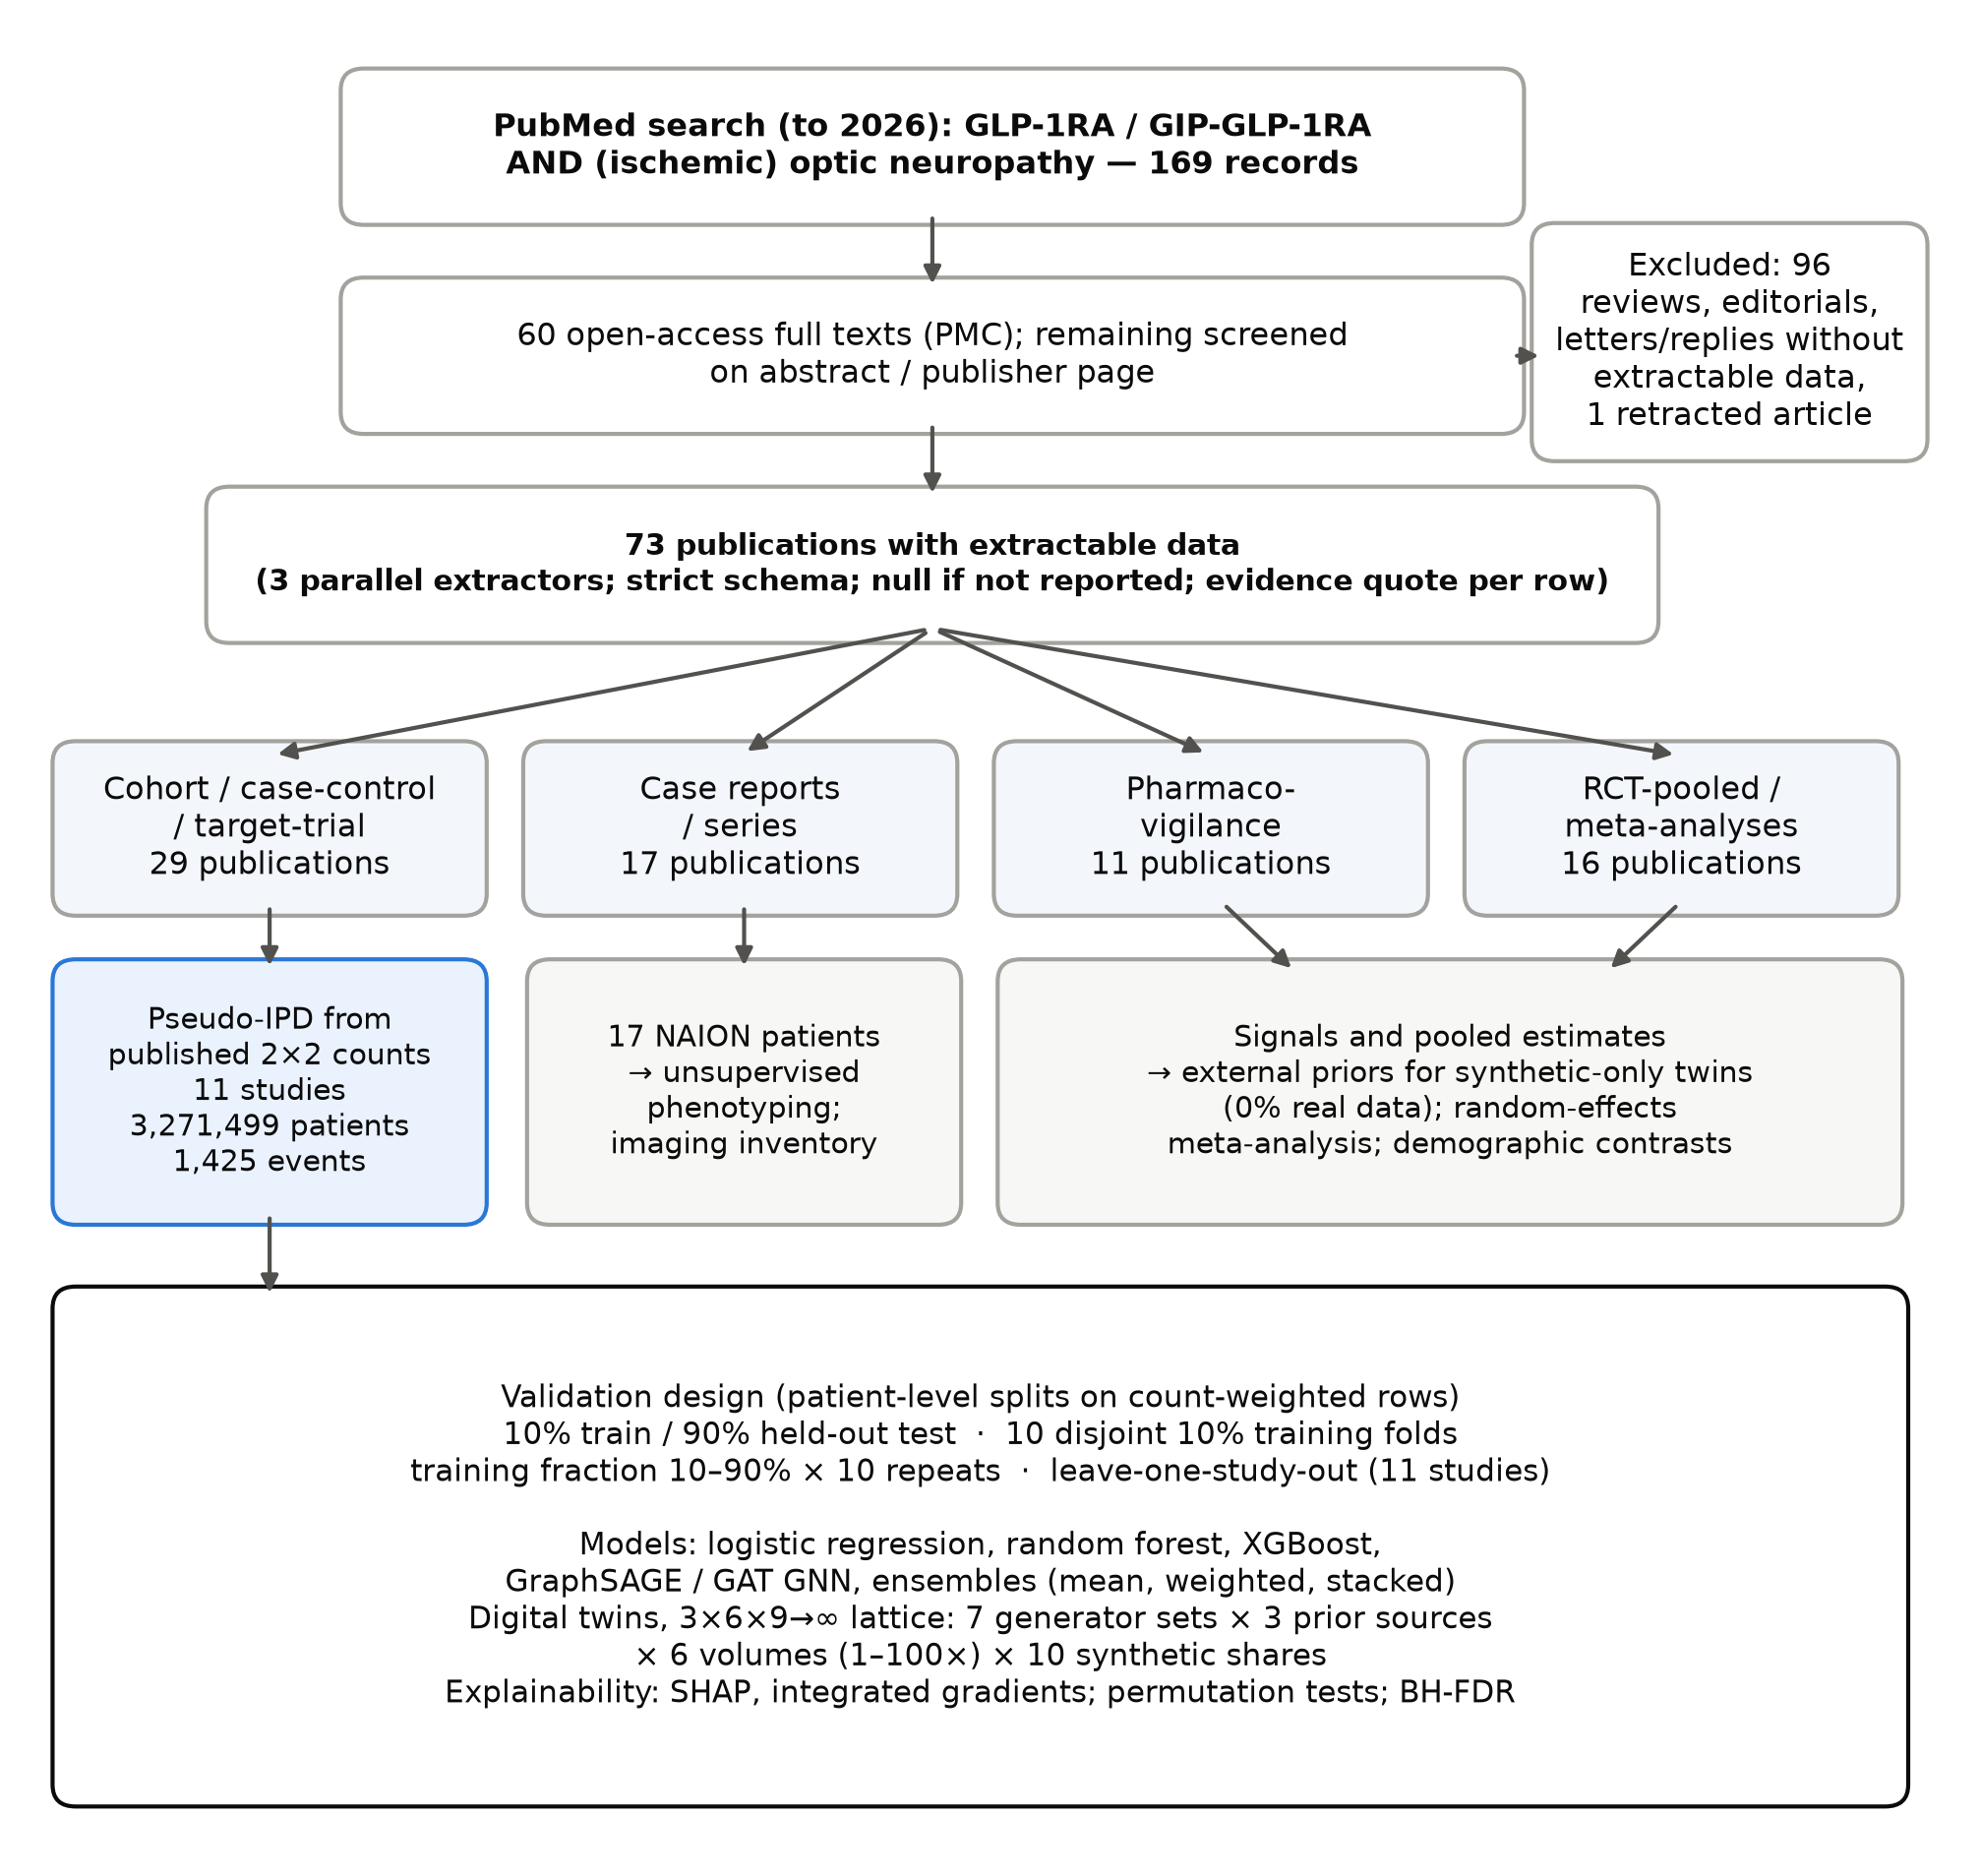
\includegraphics[width=1\linewidth,height=\textheight,keepaspectratio,alt={Study flow and validation design. Boxes show the PubMed search, screening of PubMed Central full texts, structured extraction by publication type, reconstruction of count-weighted pseudo-individual patient data from published 2x2 counts, and the validation schemes (10\% train / 90\% test hold-out, ten disjoint 10\% training folds, training fractions of 10\% to 90\%, leave-one-study-out) applied to all models. Remaining abbreviations and variable names: Nomenclature appendix.}]{figures/fig1_study_flow.png}
\caption{Study flow and validation design. Boxes show the PubMed search,
screening of PubMed Central full texts, structured extraction by
publication type, reconstruction of count-weighted pseudo-individual
patient data from published 2x2 counts, and the validation schemes (10\%
train / 90\% test hold-out, ten disjoint 10\% training folds, training
fractions of 10\% to 90\%, leave-one-study-out) applied to all models.
Remaining abbreviations and variable names: Nomenclature
appendix.}\label{fig:flow}
\end{figure*}

\subsection{Associations}\label{associations}

With study fixed effects, GLP-1RA exposure was associated with NAION
(odds ratio 1.59 (95\% CI, 1.42 to 1.77); q\textless0.001). Estimates
were 1.73 (95\% CI, 1.44 to 2.08) for semaglutide, 2.70 (95\% CI, 1.64
to 4.44) when the indication was obesity and 1.62 (95\% CI, 1.45 to
1.82) for type 2 diabetes. The association depended on the comparator:
1.81 (95\% CI, 1.54 to 2.11) against SGLT2 inhibitors and 2.35 (95\% CI,
1.74 to 3.16) against other antidiabetic drugs, but 1.03 (95\% CI, 0.57
to 1.85) against DPP-4 inhibitors and 1.14 (95\% CI, 0.94 to 1.39)
against untreated comparators. In patients with idiopathic intracranial
hypertension the direction reversed (0.43 (95\% CI, 0.22 to 0.84)). The
exposure effect was larger in studies with older participants
(interaction odds ratio 1.99 (95\% CI, 1.30 to 3.04) per 10 years;
q=0.002) and did not vary with the percentage of women (q=0.943).
Random-effects pooling of published estimates gave a ratio of 1.34 (95\%
CI, 1.16 to 1.55; I\textsuperscript{2} = 87\%) (Fig.~\ref{fig:forestpub}). Patients in
case reports were younger than exposed cohort participants (median 47 vs
60 years; q=0.016); the excess of men was not significant (q=0.274).

\subsection{Discrimination, calibration and
explainability}\label{discrimination-calibration-and-explainability}

Trained on 10\% of patients, XGBoost reached an AUROC of 0.657 on the
remaining 90\% with calibration slope 0.97; across ten disjoint 10\%
training folds the AUROC was 0.656 \ensuremath{\pm} 0.011 and O/E 1.00
(Fig.~\ref{fig:roc}). Logistic regression (0.616) and random forest
(0.646) did not differ significantly from XGBoost (all corrected
q\ensuremath{\geq}0.27). AUROC rose with training fraction to a plateau near 0.67 at
40\% to 60\%. In unseen studies, AUROC fell to 0.534. SHAP rankings were
stable across folds; permutation tests confirmed signal for exposure
(q=0.004) and therapy (q=0.015), while data source and region ---
markers of setting rather than patient risk --- carried the largest
attributions.

\begin{figure*}[!t]
\centering
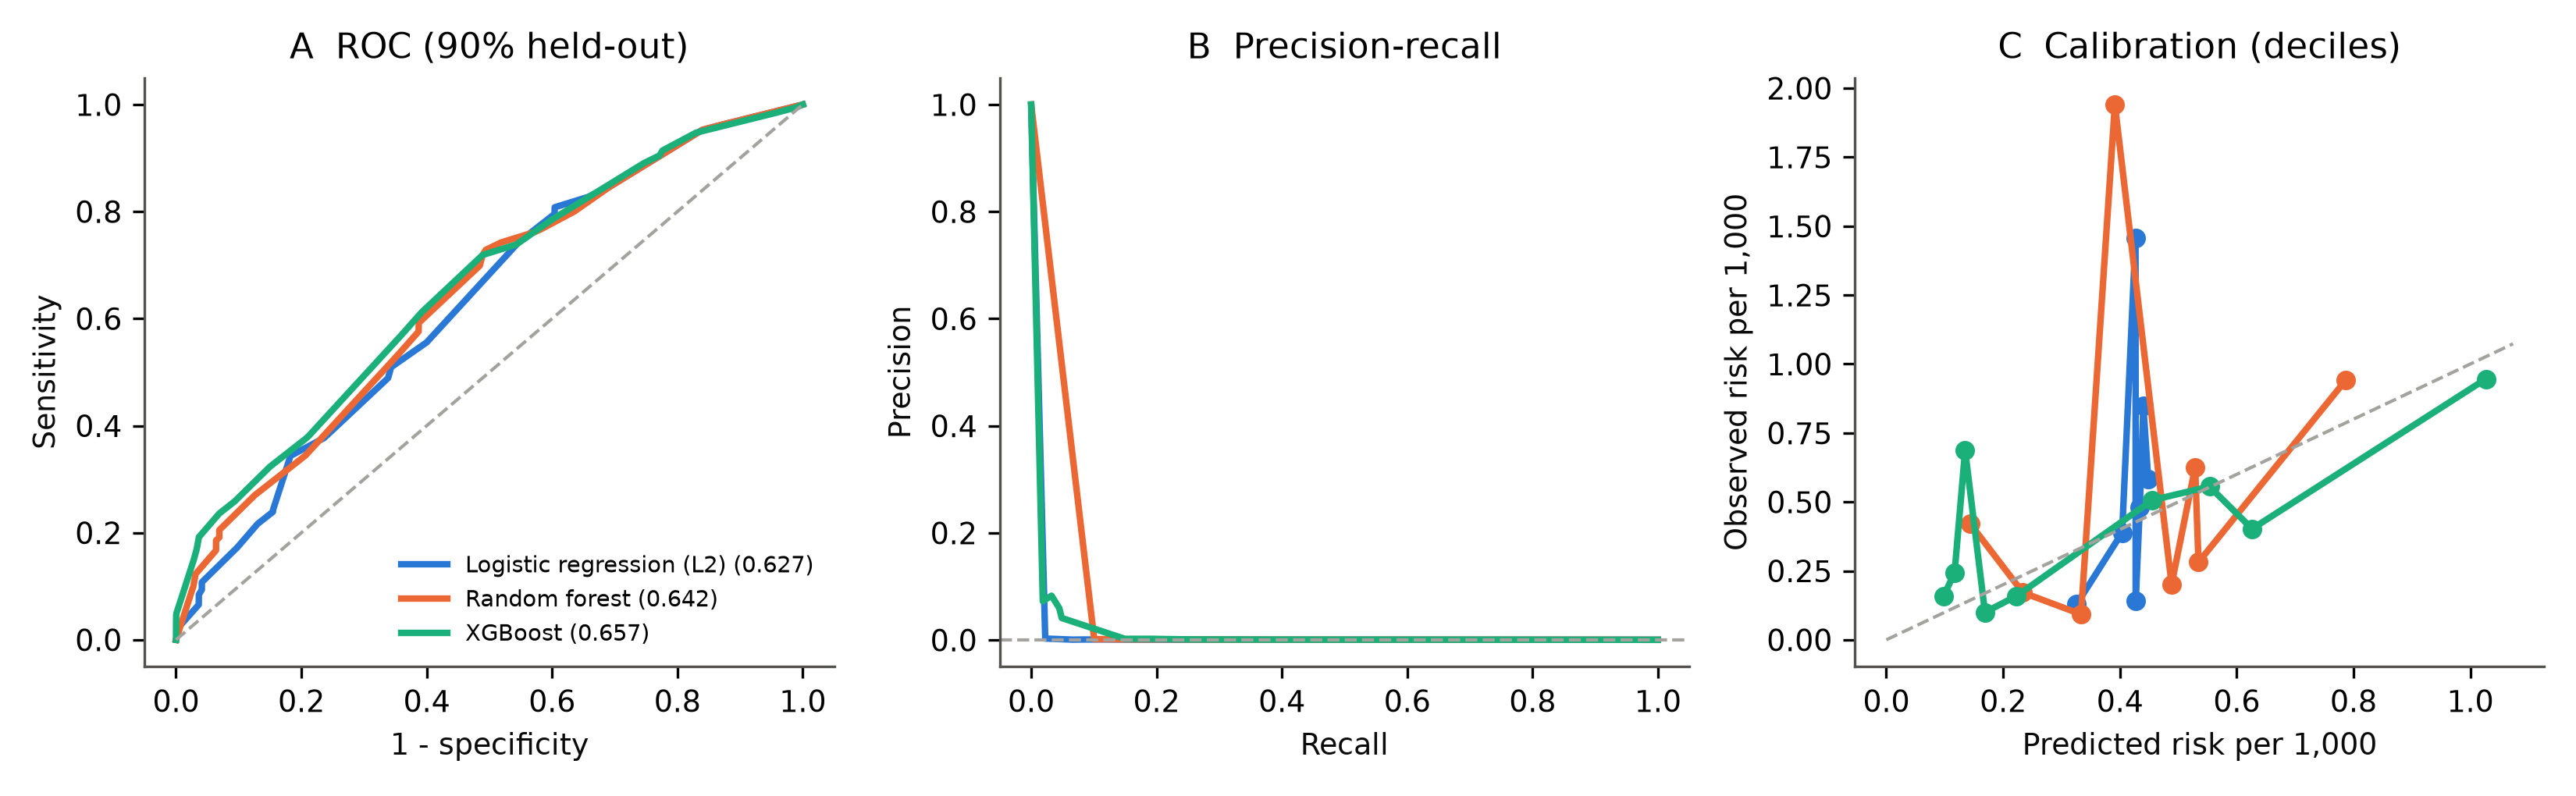
\includegraphics[width=1\linewidth,height=\textheight,keepaspectratio,alt={Discrimination and calibration of PubMed-only models on the 90\% hold-out (trained on 10\%). (A) Receiver operating characteristic curves; AUROC in the legend; dashed diagonal = chance. (B) Precision-recall curves; precision is bounded by the NAION prevalence (0.044\%), so curves fall close to zero. (C) Calibration by decile of predicted risk: predicted versus observed NAION risk per 1,000 patients; dashed line = perfect calibration. Blue, logistic regression (L2); orange, random forest; green, XGBoost. Remaining abbreviations and variable names: Nomenclature appendix.}]{figures/fig_holdout_roc_pr_cal.png}
\caption{Discrimination and calibration of PubMed-only models on the
90\% hold-out (trained on 10\%). (A) Receiver operating characteristic
curves; AUROC in the legend; dashed diagonal = chance. (B)
Precision-recall curves; precision is bounded by the NAION prevalence
(0.044\%), so curves fall close to zero. (C) Calibration by decile of
predicted risk: predicted versus observed NAION risk per 1,000 patients;
dashed line = perfect calibration. Blue, logistic regression (L2);
orange, random forest; green, XGBoost. Remaining abbreviations and
variable names: Nomenclature appendix.}\label{fig:roc}
\end{figure*}

\subsection{Threshold performance}\label{threshold-performance}

At the top-10\% threshold, XGBoost had sensitivity 0.35, specificity
0.82, PPV 0.087\% and NPV 99.97\% (positive likelihood ratio 2.01); at
the Youden threshold sensitivity was 0.59 and specificity 0.61.
Sensitivity and PPV exceeded chance (P\textless0.001), whereas
specificity did not exceed the value expected at the same flag rate and
accuracy remained below the no-information rate of 99.96\%. Net benefit
exceeded treat-all and treat-none strategies only at threshold
probabilities below 0.1\%. No metric differed between models (all
q\ensuremath{\geq}0.99).

\subsection{Graph neural networks, ensembles and digital
twins}\label{graph-neural-networks-ensembles-and-digital-twins}

The GraphSAGE GNN reached an AUROC of 0.649 \ensuremath{\pm} 0.014 across the 10 folds,
not different from XGBoost on identical splits (difference -0.0077;
P=0.779), with O/E 1.01. In leave-one-study-out validation its AUROC was
0.531 (P=0.034 vs 0.5). Integrated-gradient attributions ranked therapy,
data source and region highest, mirroring SHAP.

Nested tuning over 366 GNN configurations selected a SAGE network of
depth 6 with k=20 neighbours, uniform edge weighting and same-study
weight 5.0; on the untouched folds it differed from the default network
by 0.0006 AUROC (P=0.948).

Among 11 member combinations \ensuremath{\times} 3 combiners, the best ensemble
(cross\_family(pubmed+hybrid+synthetic), mean) reached AUROC 0.657, a
difference of 0.0010 from the best single model (q=1.000).

In the XGBoost grid (5,310 fits), no hybrid cell improved AUROC over
PubMed-only training (0 of 162 cells with a confidence interval above
zero); the best hybrid changed AUROC by 0.0009 (95\% CI, -0.0004 to
0.0022), synthetic-only training with twins fitted to real data lost
0.010, and twins built only from published priors reached AUROC values
near 0.55. Adding twins beyond about 9 to 27 times the real training
size reduced performance.

Across the full factorial grid (45,360 configurations), 4452 hybrid or
synthetic configurations improved discrimination over PubMed-only
training after Benjamini-Hochberg correction.

Table~\ref{tbl:models} summarizes the main model families.

\subsection{Transport, fine-tuning and convolutional
networks}\label{transport-fine-tuning-and-convolutional-networks}

\textbf{Background-risk model transported to GLP-1RA users.} Trained on
1,983,956 non-GLP patients (740 events), background models discriminated
within non-users (AUROC 0.626 to 0.666) but much less among 1,287,543
GLP-1RA users (685 events): AUROC 0.533 to 0.597 (best, ensemble).
Observed events among GLP-1RA users exceeded background predictions (O/E
1.41 to 1.63), an independent estimate of excess risk consistent with
the within-study odds ratio. Traditional and setting features therefore
explain little of which GLP-1RA users develop NAION.

\textbf{Fine-tuning.} The best update (pooled refit; pretraining
synthetic, fine-tuning hybrid, 10\% of GLP-1RA patients) reached AUROC
0.618 in held-out GLP-1RA users with O/E 1.08. 49 configurations
improved on the pretrained background model after Benjamini-Hochberg
correction. Recalibration corrected under-prediction without changing
discrimination, as expected; synthetic fine-tuning data did not
outperform real data.

\textbf{Convolutional network.} The 1D-CNN reached AUROC 0.653 \ensuremath{\pm} 0.011
across ten folds, not different from XGBoost (difference -0.0037;
P=0.782), and 0.514 in leave-one-study-out validation. Convolutions add
nothing when features lack spatial or sequential structure. Two- and
three-dimensional CNNs and multimodal fusion were not trainable: the
corpus contains one usable modality (structured tabular data derived
from text), imaging only as published figures for about six patients,
and no video.

\subsection{Incidence, rare-event and anomaly
models}\label{incidence-rare-event-and-anomaly-models}

\textbf{Incidence.} NAION occurred at 32.0 per 100,000 person-years
among GLP-1RA users and 17.9 among comparators (incidence rate ratio
1.79; 95\% CI, 1.61 to 1.99; Mantel-Haenszel ratio stratified by study
1.73), a rate difference of 14.1 per 100,000 person-years. Both rates
lie within or above the published background range for adults aged 50
years or older \cite{p8032479, p9186104}. The ratio was 1.84 in type 2
diabetes and 0.43 in idiopathic intracranial hypertension, and Poisson
models with study fixed effects showed heterogeneity of the exposure
effect by study age band (P=\textless0.001), indication
(P=\textless0.001), drug (P=0.002), comparator (P=0.026) and follow-up
(P=\textless0.001) but not by the percentage of women (P=0.756). Because
age is a study-level attribute and person-years were reported by only
two studies, these strata describe settings rather than individual
patients.

\textbf{Rare-event and anomaly-detection models.} A Poisson rate model
with a person-time offset (AUROC 0.652), King-Zeng corrected logistic
regression (0.655) and incidence-anchored XGBoost (0.657) matched
standard XGBoost (0.656); class weighting required prior correction to
restore calibration, and a focal-loss network was miscalibrated. Anomaly
detectors trained only on patients without NAION performed near chance
(AUROC 0.413 to 0.575), because patients with and without NAION from the
same study arm share identical features in reconstructed aggregate data;
anomaly methods need individual-level covariates.

\begin{table*}[!htbp]\centering\caption{NAION incidence per 100,000 person-years (rate) in GLP-1RA users and
comparators by stratum. Events = NAION events; IRR = incidence rate
ratio (GLP-1RA / comparator) with exact conditional binomial 95\% CI; MH
IRR = Mantel-Haenszel IRR pooled within studies; q = Benjamini-Hochberg
adjusted P value. Rates are per 100,000 person-years; Study mean age,
Women in study and Follow-up are study-level bands; T2D, type 2
diabetes; IIH, idiopathic intracranial hypertension. Remaining
abbreviations and variable names: Nomenclature appendix.}\scriptsize
\maxwbox{\textwidth}{\begin{tabular}{llllllllllll}\toprule
Stratifier & Level & Studies & GLP events & GLP rate & Non-GLP events & Non-GLP rate & IRR & 95\% CI low & 95\% CI high & MH IRR & q \\
\midrule
Overall & All studies & 11 & 685 & 32.0 & 740 & 17.9 & 1.79 & 1.61 & 1.99 & 1.73 & \textless0.001 \\
Study mean age & \textless55 y & 1 & 12 & 37.6 & 28 & 87.8 & 0.43 & 0.20 & 0.87 & 0.43 & 0.023 \\
Study mean age & 55-59 y & 4 & 206 & 16.4 & 270 & 18.7 & 0.88 & 0.73 & 1.06 & 1.47 & 0.194 \\
Study mean age & 60 y or older & 1 & 270 & 103.5 & 144 & 55.2 & 1.88 & 1.53 & 2.31 & 1.88 & \textless0.001 \\
Study mean age & Not reported & 5 & 197 & 33.1 & 298 & 12.4 & 2.66 & 2.21 & 3.20 & 2.13 & \textless0.001 \\
Women in study & \textless40\% & 1 & 30 & 122.9 & 143 & 66.5 & 1.85 & 1.20 & 2.75 & 1.85 & 0.005 \\
Women in study & 40-54\% & 5 & 513 & 28.8 & 422 & 13.6 & 2.12 & 1.86 & 2.42 & 1.76 & \textless0.001 \\
Women in study & 55\% or more & 2 & 58 & 172.8 & 51 & 144.5 & 1.20 & 0.81 & 1.78 & 1.71 & 0.432 \\
Women in study & Not reported & 3 & 84 & 28.1 & 124 & 16.0 & 1.75 & 1.31 & 2.33 & 1.52 & \textless0.001 \\
Follow-up & 1 y or less & 3 & 346 & 72.8 & 261 & 30.2 & 2.41 & 2.04 & 2.84 & 1.74 & \textless0.001 \\
Follow-up & 1-2.5 y & 4 & 173 & 29.5 & 269 & 34.6 & 0.85 & 0.70 & 1.04 & 1.27 & 0.123 \\
Follow-up & \textgreater2.5 y & 4 & 166 & 15.4 & 210 & 8.4 & 1.83 & 1.48 & 2.25 & 2.43 & \textless0.001 \\
Indication & IIH & 1 & 12 & 37.6 & 28 & 87.8 & 0.43 & 0.20 & 0.87 & 0.43 & 0.023 \\
Indication & T2D & 10 & 673 & 31.9 & 712 & 17.4 & 1.84 & 1.65 & 2.05 & 1.81 & \textless0.001 \\
Drug & GLP-1RA class & 5 & 454 & 51.8 & 368 & 29.1 & 1.78 & 1.55 & 2.05 & 1.50 & \textless0.001 \\
Drug & Semaglutide or tirzepatide & 1 & 35 & 22.0 & 19 & 11.9 & 1.84 & 1.03 & 3.41 & 1.84 & 0.052 \\
Drug & Semaglutide & 5 & 196 & 17.8 & 353 & 13.0 & 1.36 & 1.14 & 1.63 & 2.29 & 0.001 \\
Comparator & DPP-4i & 1 & 14 & 13.1 & 53 & 12.7 & 1.03 & 0.53 & 1.88 & 1.03 & 0.880 \\
Comparator & No GLP-1RA & 3 & 175 & 25.1 & 258 & 12.8 & 1.97 & 1.62 & 2.40 & 1.44 & \textless0.001 \\
Comparator & Other antidiabetic & 3 & 126 & 14.7 & 71 & 8.2 & 1.78 & 1.32 & 2.41 & 2.25 & \textless0.001 \\
Comparator & SGLT2i & 4 & 370 & 77.6 & 358 & 43.0 & 1.80 & 1.56 & 2.09 & 1.84 & \textless0.001 \\
Region & Nordic & 3 & 137 & 28.2 & 222 & 11.2 & 2.51 & 2.01 & 3.12 & 2.07 & \textless0.001 \\
Region & UK & 1 & 14 & 13.1 & 53 & 12.7 & 1.03 & 0.53 & 1.88 & 1.03 & 0.880 \\
Region & US & 7 & 534 & 34.5 & 465 & 26.7 & 1.29 & 1.14 & 1.47 & 1.67 & \textless0.001 \\
Data source & Claims & 1 & 270 & 103.5 & 144 & 55.2 & 1.88 & 1.53 & 2.31 & 1.88 & \textless0.001 \\
Data source & EHR network & 4 & 188 & 14.9 & 155 & 12.3 & 1.21 & 0.98 & 1.51 & 1.21 & 0.094 \\
Data source & Primary-care EHR & 1 & 14 & 13.1 & 53 & 12.7 & 1.03 & 0.53 & 1.88 & 1.03 & 0.880 \\
Data source & National registry & 3 & 137 & 28.2 & 222 & 11.2 & 2.51 & 2.01 & 3.12 & 2.07 & \textless0.001 \\
Data source & Single center & 1 & 46 & 2762.8 & 23 & 676.1 & 4.09 & 2.43 & 7.06 & 4.09 & \textless0.001 \\
Data source & VA EHR & 1 & 30 & 122.9 & 143 & 66.5 & 1.85 & 1.20 & 2.75 & 1.85 & 0.005 \\
\bottomrule\end{tabular}}
\end{table*}

\subsection{Detection within GLP-1RA users and
non-users}\label{detection-within-glp-1ra-users-and-non-users}

\textbf{Performance within GLP-1RA users and within non-users.} Trained
on mixed data, every model discriminated better among non-users (AUROC
0.577 to 0.674) than among GLP-1RA users (0.511 to 0.600; best, xgb).
The within-group difference in AUROC was significant after correction
for 0 of 9 models. Together with the under-prediction of a background
model in GLP-1RA users, this indicates that the features available in
published data capture background NAION risk but little of what
determines which GLP-1RA users develop NAION.

\begin{table*}[!htbp]\centering\caption{Model performance within GLP-1RA users and within non-users (mean over
ten folds; threshold = top 10\% of training risk). PR-AUC = area under
the precision-recall curve; O/E = observed/expected events; Sens,
sensitivity; Spec, specificity; Acc, accuracy; PPV and NPV = positive
and negative predictive values (proportions). LR, logistic regression;
RF, random forest; XGB, XGBoost; GNN, graph neural network; CNN,
one-dimensional convolutional network; Ens., mean ensemble; Poisson,
Poisson regression with person-time offset; IForest, isolation forest;
AE, autoencoder; --- = not applicable (anomaly scores are not calibrated
probabilities). Remaining abbreviations and variable names: Nomenclature
appendix.}\scriptsize
\maxwbox{\textwidth}{\begin{tabular}{llllllllll}\toprule
Model & Group & AUROC & PR-AUC & O/E & Sens & Spec & Acc & PPV & NPV \\
\midrule
LR & GLP-1RA users & 0.5612 & 0.0008 & 1.1752 & 0.3310 & 0.7352 & 0.7350 & 0.0008 & 0.9995 \\
LR & non-users & 0.6350 & 0.0007 & 0.8887 & 0.1925 & 0.9213 & 0.9211 & 0.0012 & 0.9997 \\
RF & GLP-1RA users & 0.5902 & 0.0009 & 1.0958 & 0.3449 & 0.7536 & 0.7534 & 0.0008 & 0.9995 \\
RF & non-users & 0.6632 & 0.0008 & 0.9392 & 0.2630 & 0.9181 & 0.9178 & 0.0015 & 0.9997 \\
XGB & GLP-1RA users & 0.5995 & 0.0062 & 1.0111 & 0.3937 & 0.7106 & 0.7104 & 0.0008 & 0.9995 \\
XGB & non-users & 0.6740 & 0.0017 & 1.0089 & 0.3150 & 0.8917 & 0.8914 & 0.0014 & 0.9997 \\
GNN & GLP-1RA users & 0.5942 & 0.0061 & 1.0097 & 0.3943 & 0.7060 & 0.7059 & 0.0008 & 0.9995 \\
GNN & non-users & 0.6673 & 0.0015 & 1.0100 & 0.3099 & 0.8911 & 0.8909 & 0.0014 & 0.9997 \\
CNN & GLP-1RA users & 0.5946 & 0.0060 & 1.0018 & 0.3845 & 0.7143 & 0.7141 & 0.0008 & 0.9995 \\
CNN & non-users & 0.6731 & 0.0017 & 0.9998 & 0.3112 & 0.8918 & 0.8916 & 0.0014 & 0.9997 \\
Ens. & GLP-1RA users & 0.5977 & 0.0061 & 1.0674 & 0.3662 & 0.7374 & 0.7372 & 0.0012 & 0.9995 \\
Ens. & non-users & 0.6719 & 0.0015 & 0.9581 & 0.3150 & 0.8917 & 0.8914 & 0.0014 & 0.9997 \\
Poisson & GLP-1RA users & 0.5972 & 0.0060 & 1.0153 & 0.3636 & 0.7426 & 0.7424 & 0.0010 & 0.9996 \\
Poisson & non-users & 0.6706 & 0.0016 & 1.0112 & 0.3254 & 0.8817 & 0.8815 & 0.0013 & 0.9997 \\
IForest & GLP-1RA users & 0.5110 & 0.0006 & --- & 0.2234 & 0.7991 & 0.7988 & 0.0006 & 0.9995 \\
IForest & non-users & 0.5767 & 0.0007 & --- & 0.2405 & 0.9292 & 0.9289 & 0.0013 & 0.9997 \\
AE & GLP-1RA users & 0.5136 & 0.0037 & --- & 0.2349 & 0.8168 & 0.8165 & 0.0008 & 0.9995 \\
AE & non-users & 0.6114 & 0.0008 & --- & 0.1617 & 0.9475 & 0.9472 & 0.0012 & 0.9997 \\
\bottomrule\end{tabular}}
\end{table*}

\subsection{Vascular score features and a proposed NAION-adapted
score}\label{vascular-score-features-and-a-proposed-naion-adapted-score}

\textbf{Validated vascular score as a feature.} Only three ABCD2/ABCD3-I
items could be derived: age 60 years or older (7 of 11 studies, from
study mean age), blood pressure (5 of 11, using hypertension prevalence
as a proxy) and diabetes (11 of 11); clinical features, symptom
duration, dual events and imaging are specific to transient ischemic
attack. Adding the partial items to XGBoost changed AUROC by -0.0019
(P=0.917). The partial score alone, in studies with all items, reached
AUROC 0.545.

\textbf{Proposed NAION-adapted points score.} Fitting point weights to
the reconstructed data produced implausible protective signs for
hypertension, diabetes and GLP-1RA exposure, because these items vary
only between studies; we therefore report this fit only as a
demonstration of ecological bias. A literature-informed version assigned
points from published patient-level ratios (male sex, hypertension,
hyperlipidemia, diabetes, coronary heart disease and sleep apnea
\cite{p34671609}) and from our within-study GLP-1RA estimates
(indication-specific), with age carried from the ABCD2 convention: male
sex 2 points, hypertension 1 point, hyperlipidemia 1 point, diabetes 2
points, coronary heart disease 2 points, sleep apnea 5 points, age ge60
1 point, cdr le 0.20 post exposure fellow eye 16 points, cdr 0.21 0.40
post exposure fellow eye 8 points, glp1ra t2d 2 points, glp1ra obesity 4
points. On setting-level data it ranked cohorts poorly (AUROC 0.417;
difference from XGBoost -0.240), as expected when settings with more
vascular risk factors recorded fewer events; the score requires
prospective, patient-level calibration, including disc morphology.

\textbf{Limitations of the partial score.} only A, B and D of
ABCD2/ABCD3-I are derivable; C, duration, dual-TIA and imaging items are
TIA-specific; A and B are study-level proxies (age from study mean with
assumed SD 12; hypertension diagnosis for BP \textgreater= 140/90); A
available for 7/11 and B for 5/11 studies; remaining values imputed and
flagged; both arms of a study share the same A and B, so the score
cannot separate exposed from unexposed patients within a study; any
apparent importance reflects between-setting differences, not individual
patient risk.

\textbf{Cup-to-disc ratio.} No source reported a pre-treatment
(pre-GLP-1RA) cup-to-disc ratio. In the case reports, disc status was
recorded at or after NAION diagnosis, usually in the unaffected fellow
eye. The largest source, a 16-center case-control study of 1,812
unaffected fellow eyes, found a fellow-eye ratio of 0.20 or less in 54\%
of patients with NAION versus 9\% of controls (odds ratio 46.3; 95\% CI,
22.9 to 93.4; ratio 0.21 to 0.40: 6.8; 3.5 to 13.2) and no difference
between semaglutide users, other GLP-1RA users and unexposed patients
\cite{p42556433}. We therefore entered the cup-to-disc ratio as the
highest-weighted item of the proposed score but labelled it a
post-exposure fellow-eye measurement: disc anatomy is structurally
stable and the fellow eye is the accepted proxy, yet this is weaker
evidence than a baseline measured before GLP-1RA initiation, and it
could not be validated in the cohort data. The same limitation applies
to NAION without GLP-1RA exposure: the classic and recent disc-at-risk
studies measured the cup-to-disc ratio after the event, in fellow eyes
or in affected eyes after edema resolved
\cite{p6514298, p3684223, p38211825, p42556433}, and none had a
measurement taken before NAION. Because both groups share this
post-event design, the comparison between exposed and unexposed NAION is
balanced, but no source supports a truly prospective (pre-event)
estimate of disc-related risk. Baseline optic disc photography or OCT
before GLP-1RA initiation in a prospective cohort would close this gap.

\textbf{With versus without ABCD features across all experiments.} Over
455 paired comparisons using identical splits and seeds, adding the
partial ABCD items changed AUROC by 0.0016 on average; 0 comparisons
differed after Benjamini-Hochberg correction.

\emph{(Table in Appendix, "Long result tables".)}

\subsection{Restriction to cohorts reporting vascular risk
factors}\label{restriction-to-cohorts-reporting-vascular-risk-factors}

No study reported medical history for individual patients, so
hypertension, sleep apnea and other NAION risk factors could not be
modelled per patient. As a sensitivity analysis we restricted the
within-study analysis to cohorts that reported these risk factors at
study level (hypertension prevalence 48-86\%, sleep apnea 13-42\%), in
which users and comparators were matched on them by design. The
association persisted and was, if anything, stronger: OR 1.79 (95\% CI,
1.55 to 2.07) in the 5 cohorts reporting hypertension (1,846,211
patients, 786 events), OR 2.02 (95\% CI, 1.70 to 2.38) in the 4 also
reporting sleep apnea, and OR 1.67 (95\% CI, 1.45 to 1.92) in the 6
cohorts with 1:1 or 1:2 propensity-score matching, compared with OR 1.59
(95\% CI, 1.42 to 1.77) overall (all P\textless0.001; Mantel-Haenszel
estimates agreed within 0.03). Discrimination was not better in these
subsets (XGBoost AUROC 0.613 to 0.631), because study-level prevalences
are balanced between arms and carry no information about which patient
develops NAION.

\begin{table*}[!htbp]\centering\caption{Sensitivity analysis restricted to cohorts reporting NAION risk-factor
prevalence at study level (hypertension; hypertension and obstructive
sleep apnea; 1:1 or 1:2 propensity-score matching). OR = within-study
odds ratio for GLP-1RA exposure (count-weighted logistic regression with
study fixed effects) with 95\% CI; MH OR = Mantel-Haenszel odds ratio;
I2 = between-study heterogeneity; XGBoost AUROC = mean over ten disjoint
10\% training folds. Remaining abbreviations and variable names:
Nomenclature appendix.}\scriptsize
\maxwbox{\textwidth}{\begin{tabular}{llllllllll}\toprule
Cohorts included & Cohorts & Patients & Events & OR & 95\% CI low & 95\% CI high & MH OR & I2 (\%) & XGBoost AUROC \\
\midrule
All cohorts & 11 & 3,271,499 & 1425 & 1.59 & 1.42 & 1.77 & 1.59 & 75.0 & 0.654 \\
Reported hypertension prevalence & 5 & 1,846,211 & 786 & 1.79 & 1.55 & 2.07 & 1.78 & 79.0 & 0.613 \\
Reported hypertension and sleep apnea prevalence & 4 & 1,476,079 & 611 & 2.02 & 1.7 & 2.38 & 1.99 & 72.0 & 0.631 \\
1:1 or 1:2 propensity-score matched & 6 & 1,877,330 & 826 & 1.67 & 1.45 & 1.92 & 1.66 & 86.0 & 0.618 \\
\bottomrule\end{tabular}}
\end{table*}

\subsection{Feature combinations and the compounding
hypothesis}\label{feature-combinations-and-the-compounding-hypothesis}

\textbf{Feature combinations and the compounding hypothesis.} Across all
511 combinations of nine feature groups, the largest Shapley
contributions to XGBoost AUROC came from setting (0.0350), duration
(0.0290), sex (0.0270), drug (0.0212). For the hypothesis that
individually negligible features contribute in combination, no feature
group met the prespecified criteria; no pair showed significant positive
interaction. For an optional-input calculator, a single XGBoost trained
with random feature-group dropout differed from a bank of dedicated
sub-models by -0.0121 AUROC on average across input patterns.

\emph{(Table in Appendix, "Long result tables".)}

\begin{table*}[!htbp]\centering\caption{Reliability of each feature's odds ratio (OR) across all combinations
containing it (count-weighted logistic regression with cluster-robust
standard errors by study). Combinations = number of feature combinations
containing the feature; Median/Min/Max OR across them; OR\textgreater1 =
share of combinations with OR above 1; q\textless0.05 = share
significant after Benjamini-Hochberg correction. Study-level covariates
are ecological and imprecise with 11 clusters. Remaining abbreviations
and variable names: Nomenclature appendix.}\scriptsize
\maxwbox{\textwidth}{\begin{tabular}{lllllll}\toprule
Feature & Combinations & Median OR & Min OR & Max OR & OR\textgreater1 & q\textless0.05 \\
\midrule
therapy\_dpp4i & 256 & 0.73 & 0.24 & 1.86 & 25\% & 100\% \\
source\_type\_single\_center & 256 & 254.36 & 0.01 & \textgreater10,000 & 99\% & 91\% \\
therapy\_other\_antiobesity & 256 & 0.19 & 0.05 & 32.57 & 16\% & 91\% \\
pct\_female & 256 & 0.61 & 0.06 & 1.42 & 13\% & 84\% \\
indication\_obesity & 256 & 34.12 & 0.11 & 182.78 & 56\% & 78\% \\
region\_uk & 256 & 0.34 & 0.01 & 49.64 & 16\% & 75\% \\
glp1ra\_exposed & 256 & 1.59 & 1.04 & 1.92 & 100\% & 74\% \\
indication\_iih & 256 & 2.99 & \textless0.01 & \textgreater10,000 & 69\% & 67\% \\
source\_type\_va\_ehr & 224 & 4.99 & \textless0.01 & 298.92 & 73\% & 65\% \\
therapy\_sglt2i & 128 & 0.58 & 0.52 & 0.97 & 0\% & 62\% \\
abcd\_D & 128 & 0.29 & 0.01 & 8.11 & 27\% & 62\% \\
abcd\_B & 256 & 1.33 & 0.96 & 8.92 & 98\% & 61\% \\
region\_nordic & 256 & 1.33 & \textless0.01 & 153.49 & 70\% & 57\% \\
outcome\_def\_ion & 216 & 1.08 & 0.16 & \textgreater10,000 & 53\% & 56\% \\
source\_type\_ehr\_network & 256 & 1.38 & \textless0.01 & 96.85 & 66\% & 50\% \\
mean\_age & 256 & \textless0.01 & \textless0.01 & \textgreater10,000 & 30\% & 44\% \\
abcd\_A & 256 & 9.69 & \textless0.01 & \textgreater10,000 & 69\% & 39\% \\
followup\_years & 256 & 0.98 & 0.67 & 22.81 & 47\% & 36\% \\
therapy\_no\_glp1ra & 256 & 0.99 & 0.86 & 1.82 & 49\% & 29\% \\
therapy\_other\_antidiabetic & 256 & 0.93 & 0.36 & 6.10 & 45\% & 12\% \\
therapy\_sema\_or\_tirz & 256 & 1.07 & 0.53 & 7.63 & 71\% & 0\% \\
therapy\_semaglutide & 256 & 1.12 & 0.77 & 2.47 & 89\% & 0\% \\
\bottomrule\end{tabular}}
\end{table*}

\subsection{Compute footprint and imaging
what-if}\label{compute-footprint-and-imaging-what-if}

\textbf{Compute, energy and token use.} All model training and inference
ran locally on one laptop (Apple M3 Pro, 11 cores, 18 GB). Across every
experiment the analyses used 7.6 wall-clock hours and 62.6 core-hours
(87\% of run time measured from logs, the rest estimated), consuming an
estimated 0.25 kWh (range 0.19 to 0.31) and emitting 92 g CO2e at the US
average grid intensity (range 19 to 215 g), about 0.5 km of car travel.
The largest single consumer was the full-factorial twins (2.4 h).
Inference was negligible: logreg 0.75 ms, rf 26.68 ms, xgb 1.69 ms per
1,000 patients. The AI assistant used for retrieval, extraction and
drafting consumed at least 764,562 tokens in the four metered extraction
and literature agents; tokens of the main session were not metered, and
assistant inference energy, which occurs in remote data centres, is not
included in these totals.

\textbf{What-if: adding ocular imaging (simulation).} Imaging values
were simulated for the reconstructed patients conditional on their
observed outcome. Adding cup-to-disc ratio from fundus photographs, with
published odds ratios \cite{p42556433} and 25\% photographic
misclassification, raised AUROC from 0.653 to 0.770; OCT-measured ratio
reached 0.818. Adding hypothetical effects for optic disc drusen, OCT
angiography perfusion and serial on-treatment imaging reached 0.840
(range across hypothetical effect sizes 0.825 to 0.876), and 0.854 with
sleep apnoea added; sleep apnoea alone reached 0.708. Positive
predictive value at the top-10\% threshold rose from 0.098\% to 0.262\%,
still below 1\% because NAION is rare. A prospective cohort would need
about 263 NAION events, roughly 604,000 GLP-1RA initiators at the
observed incidence, to estimate AUROC within \ensuremath{\pm}0.03; a case-control
design enriched for NAION would need far fewer imaged patients. These
figures are simulations that assume conditional independence of features
and, for drusen, OCT angiography and serial imaging, effect sizes that
have not been measured.

\begin{figure*}[!t]
\centering
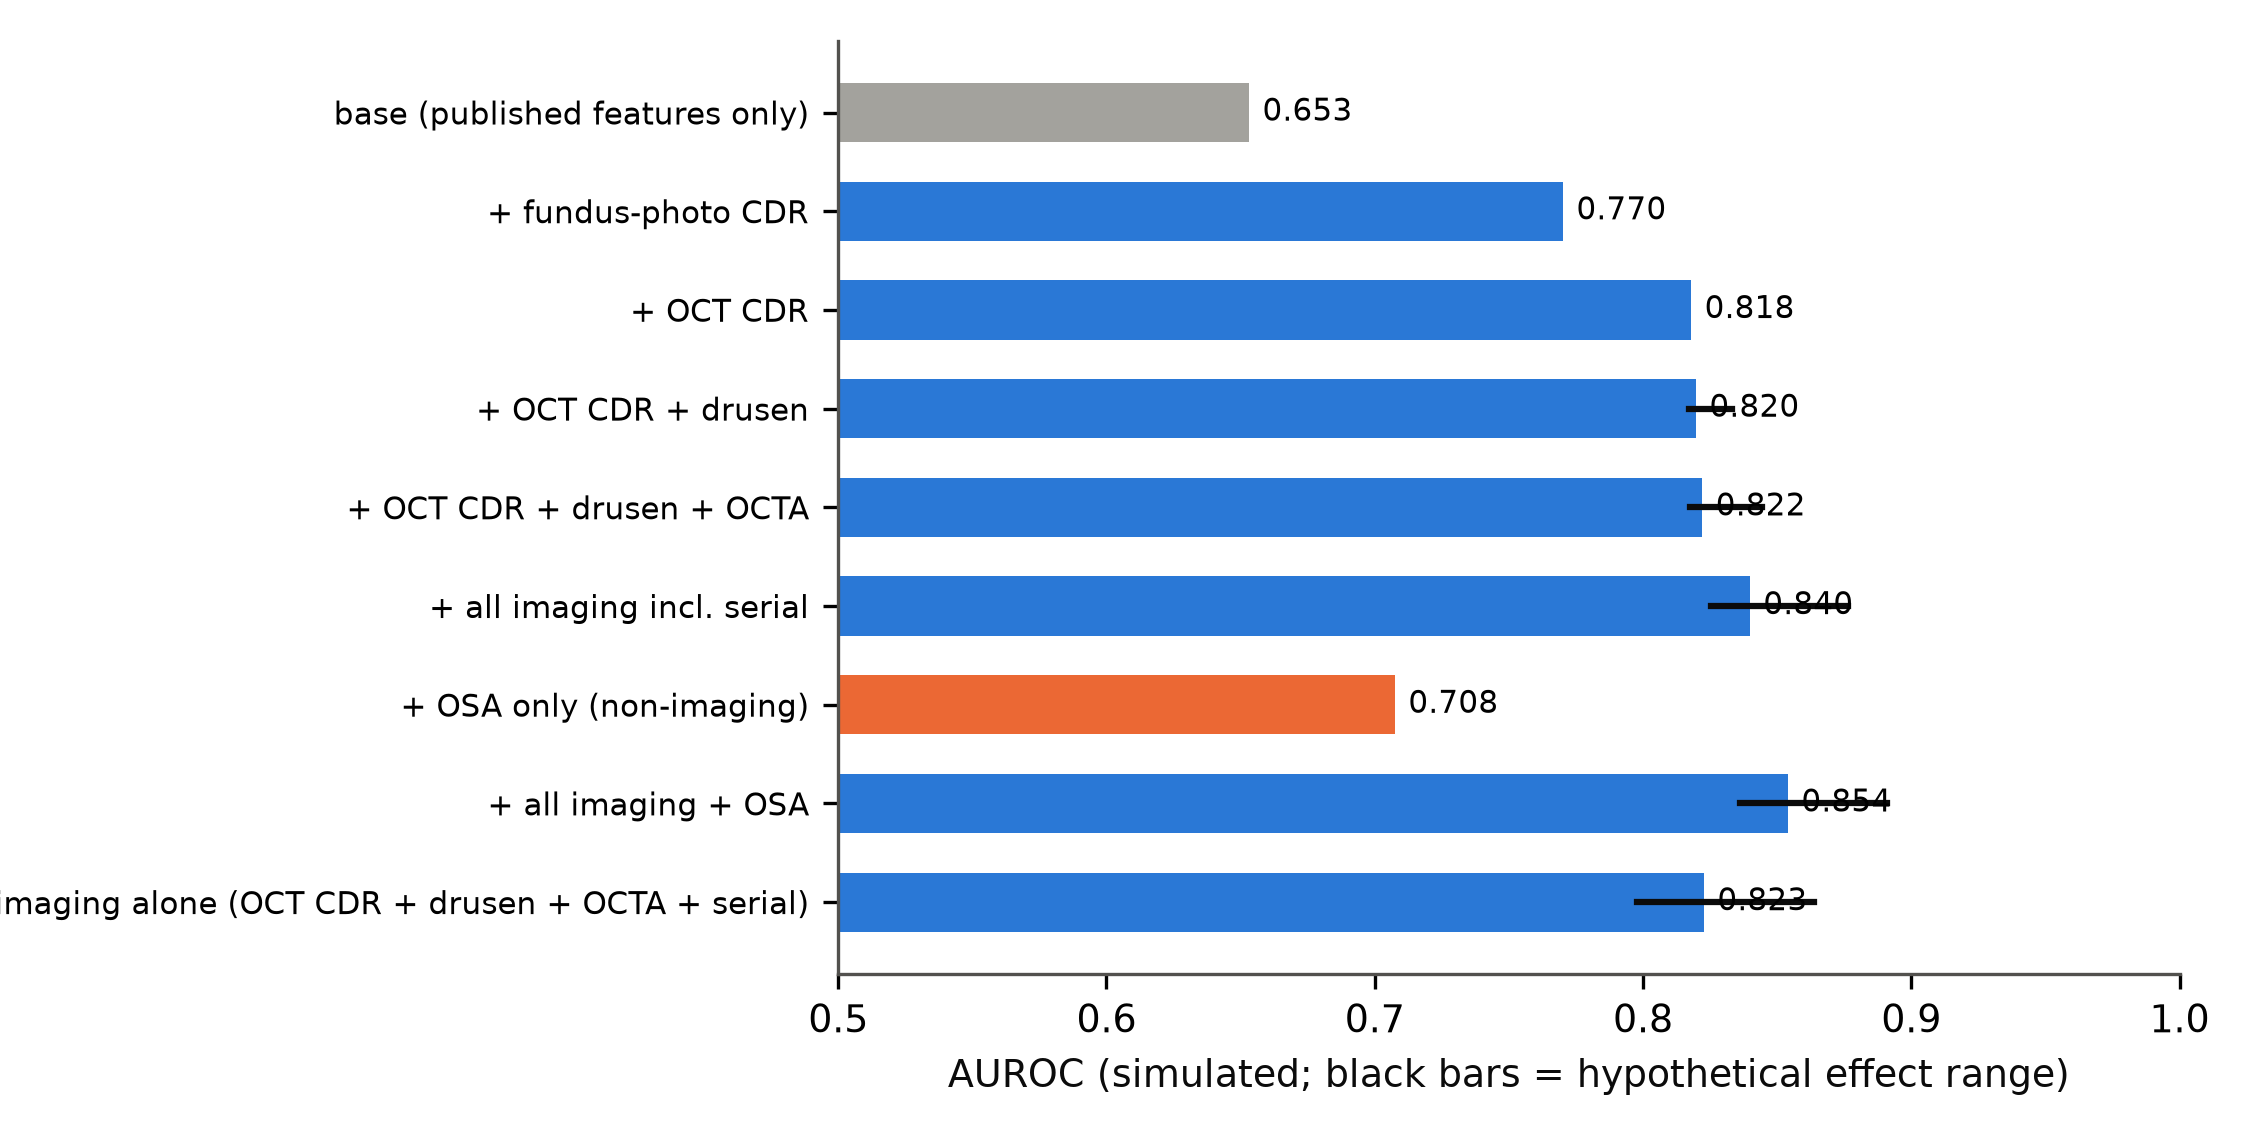
\includegraphics[width=1\linewidth,height=\textheight,keepaspectratio,alt={Simulated effect of adding ocular imaging and obstructive sleep apnoea (OSA) to the published-feature XGBoost model (AUROC; values at bar ends). Grey = base model; blue = with imaging features; orange = with OSA (non-imaging comparator). CDR = cup-to-disc ratio from fundus photographs or optical coherence tomography (OCT); drusen = optic disc drusen; OCTA = OCT angiography (peripapillary perfusion); serial = on-treatment change on repeat imaging. CDR and OSA effects use published odds ratios; drusen, OCTA and serial effects are hypothetical, and black bars show the range across low and high assumed effect sizes. All imaging values are synthetic. Remaining abbreviations and variable names: Nomenclature appendix.}]{figures/fig_imaging_whatif.png}
\caption{Simulated effect of adding ocular imaging and obstructive sleep
apnoea (OSA) to the published-feature XGBoost model (AUROC; values at
bar ends). Grey = base model; blue = with imaging features; orange =
with OSA (non-imaging comparator). CDR = cup-to-disc ratio from fundus
photographs or optical coherence tomography (OCT); drusen = optic disc
drusen; OCTA = OCT angiography (peripapillary perfusion); serial =
on-treatment change on repeat imaging. CDR and OSA effects use published
odds ratios; drusen, OCTA and serial effects are hypothetical, and black
bars show the range across low and high assumed effect sizes. All
imaging values are synthetic. Remaining abbreviations and variable
names: Nomenclature appendix.}
\end{figure*}

\begin{figure*}[!t]
\centering
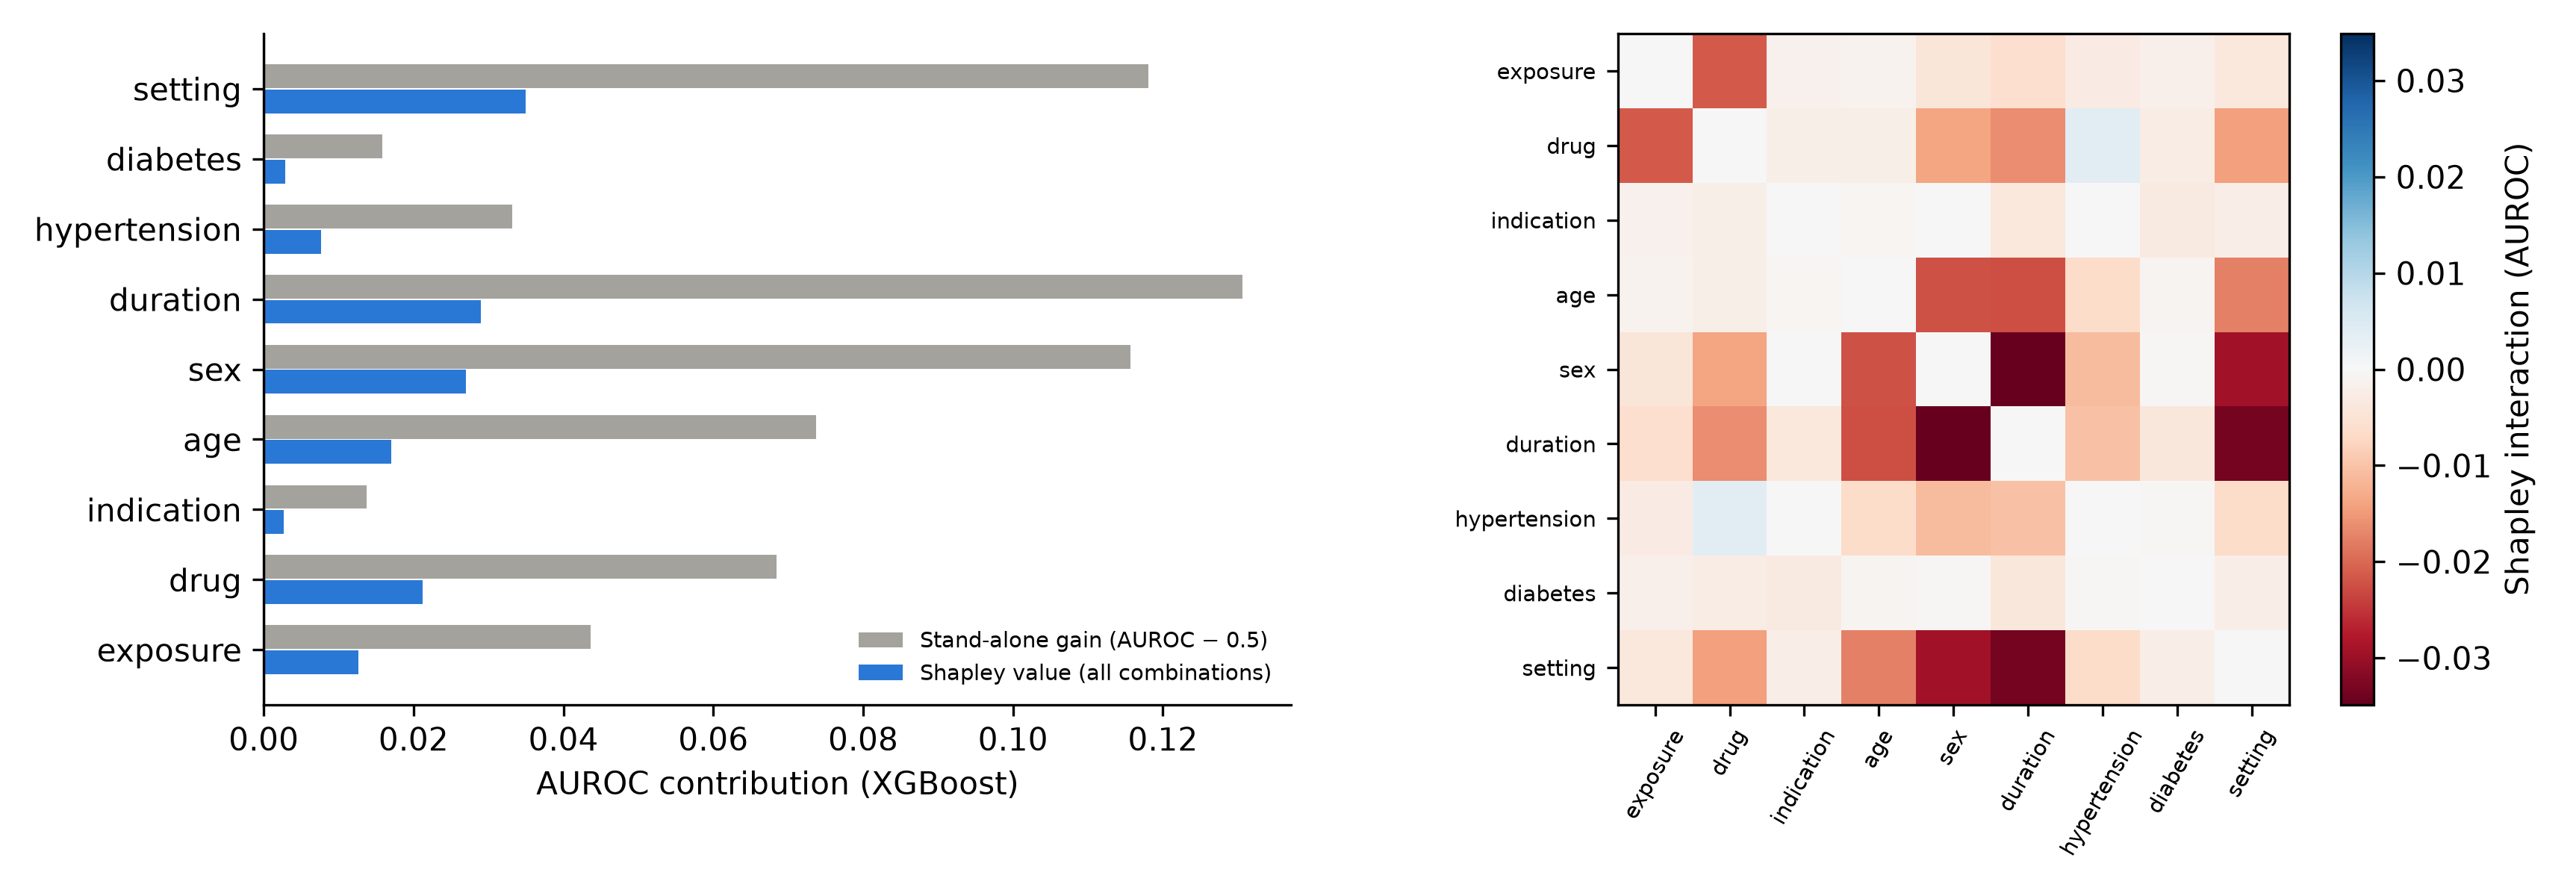
\includegraphics[width=1\linewidth,height=\textheight,keepaspectratio,alt={Feature-group contributions across all 511 combinations of nine feature groups (XGBoost). Left: grey = stand-alone gain (AUROC - 0.5 of a model using only that group); blue = Shapley value (average gain in AUROC when the group is added, over all combinations). Right: pairwise Shapley interaction indices (AUROC); red = redundancy (the pair adds less together than separately), blue = synergy. Groups: exposure = GLP-1RA exposure; drug = therapy arm; indication; age = study mean age (with partial ABCD2 age item); sex = share of women; duration = follow-up; hypertension and diabetes = partial ABCD2 items; setting = region, data source and outcome definition. Remaining abbreviations and variable names: Nomenclature appendix.}]{figures/fig_feature_combinations.png}
\caption{Feature-group contributions across all 511 combinations of nine
feature groups (XGBoost). Left: grey = stand-alone gain (AUROC - 0.5 of
a model using only that group); blue = Shapley value (average gain in
AUROC when the group is added, over all combinations). Right: pairwise
Shapley interaction indices (AUROC); red = redundancy (the pair adds
less together than separately), blue = synergy. Groups: exposure =
GLP-1RA exposure; drug = therapy arm; indication; age = study mean age
(with partial ABCD2 age item); sex = share of women; duration =
follow-up; hypertension and diabetes = partial ABCD2 items; setting =
region, data source and outcome definition. Remaining abbreviations and
variable names: Nomenclature appendix.}
\end{figure*}

\begin{figure*}[!t]
\centering
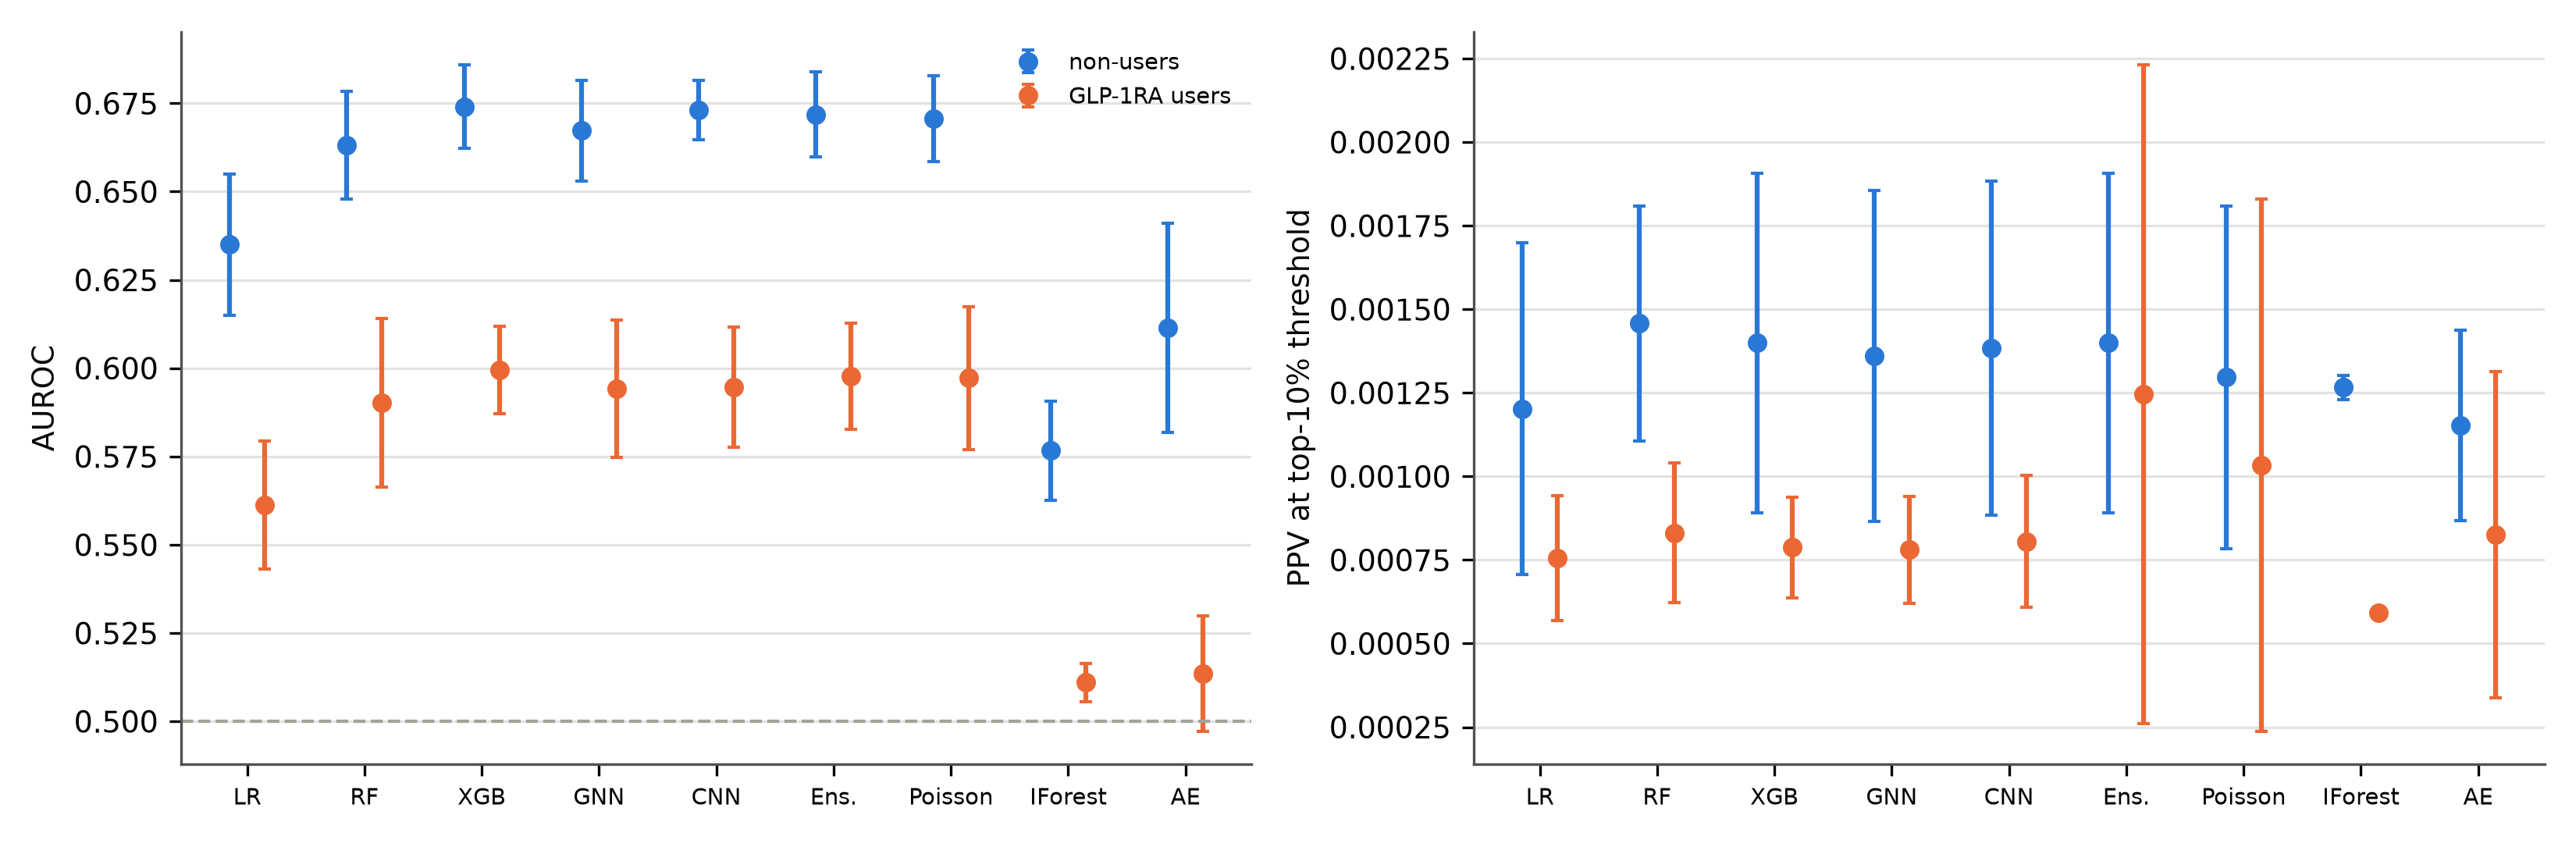
\includegraphics[width=1\linewidth,height=\textheight,keepaspectratio,alt={Detection within GLP-1RA users (orange) and within non-users (blue): (left) AUROC and (right) PPV at the threshold flagging the top 10\% of training risk (proportion; 0.001 = 0.1\%), mean \ensuremath{\pm} SD over ten folds; dashed line = AUROC 0.5. LR, logistic regression; RF, random forest; XGB, XGBoost; GNN, graph neural network; CNN, one-dimensional convolutional network; Ens., mean ensemble; Poisson, Poisson regression with person-time offset; IForest, isolation forest; AE, autoencoder (both anomaly detectors trained on non-events). Remaining abbreviations and variable names: Nomenclature appendix.}]{figures/fig_subgroups.png}
\caption{Detection within GLP-1RA users (orange) and within non-users
(blue): (left) AUROC and (right) PPV at the threshold flagging the top
10\% of training risk (proportion; 0.001 = 0.1\%), mean \ensuremath{\pm} SD over ten
folds; dashed line = AUROC 0.5. LR, logistic regression; RF, random
forest; XGB, XGBoost; GNN, graph neural network; CNN, one-dimensional
convolutional network; Ens., mean ensemble; Poisson, Poisson regression
with person-time offset; IForest, isolation forest; AE, autoencoder
(both anomaly detectors trained on non-events). Remaining abbreviations
and variable names: Nomenclature appendix.}
\end{figure*}

\begin{figure*}[!t]
\centering
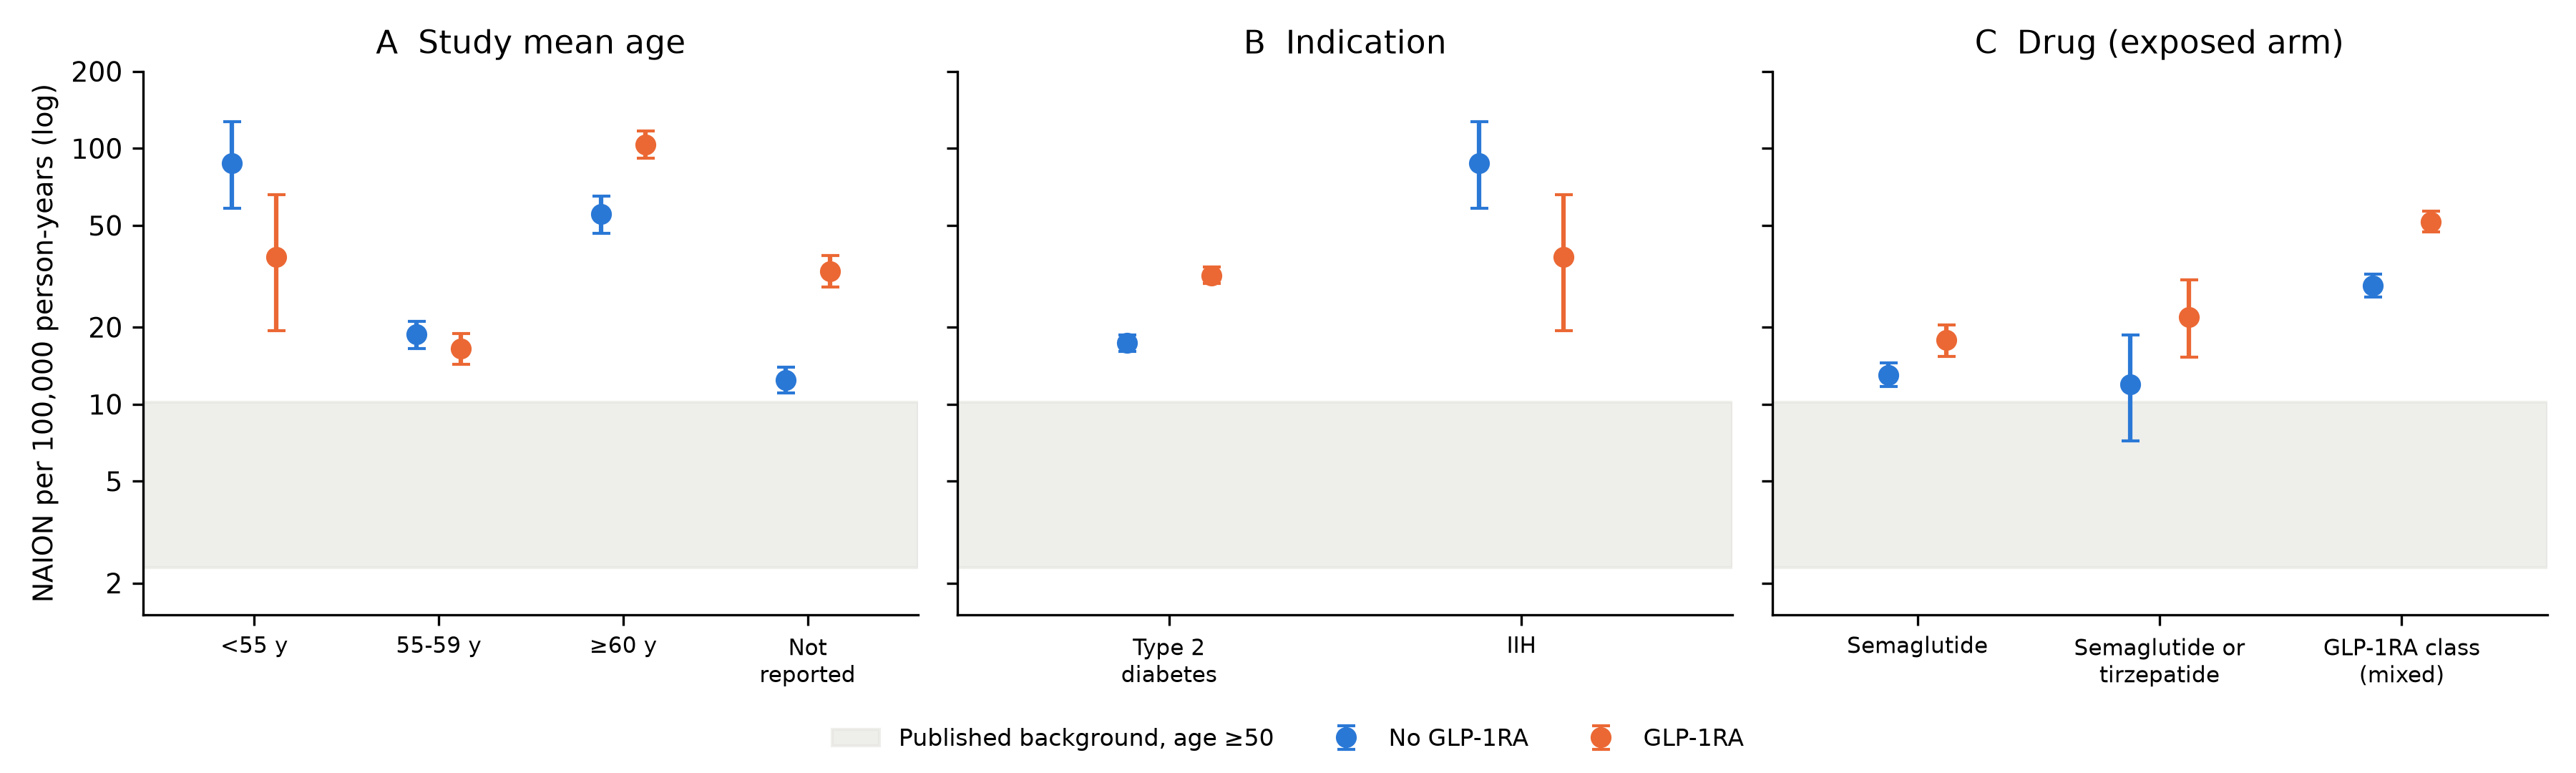
\includegraphics[width=1\linewidth,height=\textheight,keepaspectratio,alt={NAION incidence per 100,000 person-years (log scale; points = pooled rate, bars = exact Poisson 95\% CI) in GLP-1RA users (orange) and comparators (blue), by (A) study mean age band, (B) indication (IIH = idiopathic intracranial hypertension) and (C) drug of the exposed arm (GLP-1RA class = studies pooling several GLP-1RAs). Grey band = published background incidence in adults aged 50 years or older. Remaining abbreviations and variable names: Nomenclature appendix.}]{figures/fig_incidence_strata.png}
\caption{NAION incidence per 100,000 person-years (log scale; points =
pooled rate, bars = exact Poisson 95\% CI) in GLP-1RA users (orange) and
comparators (blue), by (A) study mean age band, (B) indication (IIH =
idiopathic intracranial hypertension) and (C) drug of the exposed arm
(GLP-1RA class = studies pooling several GLP-1RAs). Grey band =
published background incidence in adults aged 50 years or older.
Remaining abbreviations and variable names: Nomenclature appendix.}
\end{figure*}

\section{Discussion}\label{discussion}

Published evidence on GLP-1RAs and NAION contains a consistent exposure
signal: within the same studies, exposed patients had roughly 1.6 times
the odds of NAION, and the estimate was higher for semaglutide and for
obesity indications. Machine learning on the same evidence, however,
discriminated only modestly, and most of what it learned was where a
patient was treated rather than who the patient was. Discrimination
collapsed toward chance in studies the model had not seen, and the
strongest attributions went to data source and region. More flexible
learners --- graph neural networks, ensembles and synthetic digital
twins --- did not change this picture.

The threshold metrics show what this means in practice. Sensitivity and
PPV beat chance, so the score enriches for cases roughly twofold, which
is an advantage for selecting patients for closer surveillance or for
enrolment in research. Absolute PPV, however, stayed below 0.1\%: about
one in 1,100 flagged patients would develop NAION. Specificity added
nothing beyond the flag rate, accuracy was uninformative because the
outcome is rare, and the high NPV mainly reflected the low prevalence.
Net benefit was positive only at threshold probabilities suited to
low-risk actions such as a dilated examination or optical coherence
tomography before treatment, counselling, or slower dose escalation,
consistent with recent consensus recommendations
\cite{p42132708, p41058255}.

The intended clinical question is whether a validated score can identify
patients who should start antiplatelet therapy. These data cannot answer
it. Risk prediction is not treatment-effect prediction; none of the
extracted cohorts or case reports recorded antiplatelet exposure, NAION
is not primarily thromboembolic, and the evidence for aspirin after
NAION is limited. At the observed PPV, treating every flagged patient
would expose roughly a thousand people to bleeding risk per event that
occurs, before any benefit is assumed. Answering the question requires
prospective validation with patient-level predictors (disc morphology,
sleep apnoea, nocturnal hypotension, dose escalation) followed by a
risk-stratified trial with bleeding as a co-primary safety outcome.

Synthetic twins helped only weak learners. In the full factorial
experiment, thousands of hybrid configurations improved logistic
regression, consistent with regularization, but the best hybrid XGBoost
gained only 0.0015 AUROC; twins built from published priors alone
produced little more than chance discrimination, and fine-tuning a
background model worked only with real GLP-1RA data. Twins cannot create
patient-level information that the source data do not contain.

The limiting factor is the feature set, not the learner. In simulation,
adding cup-to-disc ratio from fundus photographs or OCT, with published
effect sizes, raised AUROC from about 0.65 to 0.77 to 0.82, and
plausible additional imaging reached about 0.84; even then positive
predictive value stayed below 1\%. A prospective cohort of GLP-1RA
initiators with baseline optic-disc imaging, which no published study
has reported, is therefore the most informative next step. The entire
analysis used about 0.25 kWh of local compute, so the environmental cost
of the modelling itself is negligible relative to the data collection it
motivates.

We describe this work as a foundation machine learning model in the
sense of a base layer: it fixes the outcome definition, the
reconstructed evidence base, the validation protocol and a benchmark
(AUROC about 0.66 within settings, about 0.53 across settings) against
which every later module must be judged. It is not a large pretrained
model. The intended next layers are encoders for optic-disc photography
and OCT and separately pretrained components such as an oculomotor world
model, a learned generative model of eye-movement dynamics adapted from
Ha and Schmidhuber \cite{ha2018}, trained on synthetic eye-movement
data and sharing no variables with the present data, combined in a
multimodal neuro-ophthalmic foundation model. No transfer between
components was performed or evaluated here; it requires patients with
linked risk factors, imaging and oculomotor recordings.

This study has limitations. Predictors were arm- or study-level, so
associations with age, sex and setting are ecological. Reconstructed
patients share covariate patterns, which makes thresholds coarse.
Outcome definitions differed (one cohort reported ischemic optic
neuropathy), TriNetX cells below 10 were masked, several studies were
available only as abstracts, and overlapping registries were handled by
selection rather than by individual linkage. No imaging was available,
so multimodal and computer-vision models could not be trained. All
results are retrospective and in silico.

\section{Conclusion}\label{conclusion}

This study asked whether published evidence can stratify the risk of
NAION in GLP-1RA users, which features carry that risk, and which model
architecture predicts it best.

\textbf{Risk features.} Within studies, GLP-1RA exposure was associated
with NAION (OR 1.59, 95\% CI 1.42 to 1.77, P\textless0.001,
q\textless0.001). The highest-risk subgroup was GLP-1RA use for obesity
(OR 2.70, 95\% CI 1.64 to 4.44, P\textless0.001, q\textless0.001),
followed by semaglutide (OR 1.73, 95\% CI 1.44 to 2.08, P\textless0.001,
q\textless0.001) and comparison with SGLT2 inhibitors (OR 1.81, 95\% CI
1.54 to 2.11, P\textless0.001, q\textless0.001); the exposure effect was
larger in studies with older participants (OR 1.99, 95\% CI 1.30 to
3.04, P=0.001, q=0.002 per 10 years of mean age). Exposure was the most
stable single feature: its odds ratio exceeded 1 in all 256 feature
combinations that contained it (median 1.59, range 1.04 to 1.92).

\textbf{Feature combinations.} The best-discriminating combination was
age + exposure + setting + sex (XGBoost, AUROC 0.660 \ensuremath{\pm} 0.008), no better
than all nine groups together (0.655 \ensuremath{\pm} 0.012). The largest contribution
came from study setting (region, data source and outcome definition;
Shapley value 0.035 AUROC, q=0.059), which describes where a patient was
studied rather than the patient; among the remaining features, the
largest contribution came from follow-up duration (time at risk)
(Shapley value 0.029 AUROC, q=0.006). No pair of feature groups was
synergistic, so the hypothesis that weak features compound into strong
risk was not supported.

\textbf{Best architecture.} PubMed-only XGBoost discriminated best
(AUROC 0.656 \ensuremath{\pm} 0.011 over ten folds), but its advantage over random
forest (+0.011 AUROC, P=0.745) and logistic regression (+0.041, P=0.218)
was not significant, and graph, convolutional, ensemble,
anomaly-detection and synthetic digital-twin variants did not improve on
it. In studies the model had not seen, AUROC fell to 0.534 (P=0.021
versus chance).

\textbf{Answer.} Published evidence supports a reproducible association
between GLP-1RA exposure and NAION, strongest with obesity indications,
but it does not support individual risk prediction good enough to select
patients for treatment, including antiplatelet therapy. The model is a
research tool for enriching cohorts, and its main product is a benchmark
and protocol for the patient-level, imaging-linked prospective data that
the question requires.

\clearpage\onecolumn
\appendices

\section{Nomenclature: abbreviations and variable
names}\label{nomenclature-abbreviations-and-variable-names}

Abbreviations are also defined at first use in the text. Variable and
label names are those printed in tables and figures; ``\ldots{}'' stands
for any suffix or prefix (for example, therapy\_\ldots{} covers
therapy\_semaglutide and therapy\_sglt2i).

{\footnotesize
\begin{longtable}[]{@{}
  >{\raggedright\arraybackslash}p{(\linewidth - 2\tabcolsep) * \real{0.5000}}
  >{\raggedright\arraybackslash}p{(\linewidth - 2\tabcolsep) * \real{0.5000}}@{}}
\caption{Abbreviations.}\tabularnewline
\toprule\noalign{}
\begin{minipage}[b]{\linewidth}\raggedright
Abbreviation
\end{minipage} & \begin{minipage}[b]{\linewidth}\raggedright
Definition
\end{minipage} \\
\midrule\noalign{}
\endfirsthead
\toprule\noalign{}
\begin{minipage}[b]{\linewidth}\raggedright
Abbreviation
\end{minipage} & \begin{minipage}[b]{\linewidth}\raggedright
Definition
\end{minipage} \\
\midrule\noalign{}
\endhead
\bottomrule\noalign{}
\endlastfoot
ABCD\textsuperscript{2} & Age, Blood pressure, Clinical features, Duration of symptoms and
Diabetes score for stroke risk after transient ischemic attack \\
ABCD\textsuperscript{3}-I & ABCD\textsuperscript{2} extended with dual transient ischemic attack and Imaging
findings \\
Acc & accuracy \\
AE & autoencoder (anomaly detector) \\
AI & artificial intelligence \\
AION & anterior ischemic optic neuropathy \\
AUROC & area under the receiver operating characteristic curve \\
B & number of permutations \\
BP & blood pressure \\
CDR & cup-to-disc ratio \\
CI & confidence interval \\
CNN & convolutional neural network (CNN-1D, one-dimensional) \\
CO2e & carbon dioxide equivalent \\
CV & cross-validation \\
DL & deep learning \\
DPP-4i & dipeptidyl peptidase-4 inhibitor \\
EBGM & empirical Bayes geometric mean (pharmacovigilance
disproportionality) \\
EHR & electronic health record \\
Ens. & ensemble (mean of member models) \\
FAERS & US Food and Drug Administration Adverse Event Reporting
System \\
FE & fixed effects \\
GAT & graph attention network \\
GB & gigabyte \\
GCIPL & ganglion cell-inner plexiform layer \\
GIP & glucose-dependent insulinotropic polypeptide \\
GLP-1 & glucagon-like peptide-1 \\
GLP-1RA & glucagon-like peptide-1 receptor agonist \\
GNN & graph neural network \\
Grad-CAM & gradient-weighted class activation mapping \\
GraphSAGE & graph sample-and-aggregate network \\
IC025 & lower 95\% credibility bound of the information component
(pharmacovigilance) \\
IForest & isolation forest (anomaly detector) \\
IIH & idiopathic intracranial hypertension \\
ION & ischemic optic neuropathy \\
IONDT & Ischemic Optic Neuropathy Decompression Trial \\
IPD & individual patient data \\
IRR & incidence rate ratio \\
I\textsuperscript{2} & percentage of between-study variance due to heterogeneity \\
k & number of estimates (meta-analysis) or neighbours per node
(graph) \\
L2 & ridge (squared-coefficient) penalty \\
LOF & local outlier factor \\
LOSO & leave-one-study-out validation \\
LR & logistic regression \\
LR+ & positive likelihood ratio \\
MH & Mantel-Haenszel \\
ML & machine learning \\
MLP & multilayer perceptron \\
MRI & magnetic resonance imaging \\
NAION & nonarteritic anterior ischemic optic neuropathy \\
NB & net benefit \\
NIR & no-information rate \\
NPV & negative predictive value \\
O/E & observed-to-expected event ratio \\
OCT & optical coherence tomography \\
OCTA & optical coherence tomography angiography \\
OR & odds ratio \\
OSA & obstructive sleep apnea \\
PC & principal component \\
PCA & principal component analysis \\
PMC & PubMed Central \\
PMID & PubMed identifier \\
PPV & positive predictive value \\
PR-AUC & area under the precision-recall curve \\
PRR & proportional reporting ratio \\
PUE & power usage effectiveness \\
PY & person-years \\
q & Benjamini-Hochberg adjusted P value \\
QPI-1007 & intravitreal small interfering RNA against caspase-2
(investigational) \\
RCT & randomized controlled trial \\
RF & random forest \\
RNFL & retinal nerve fiber layer \\
ROC & receiver operating characteristic \\
ROR & reporting odds ratio \\
SD & standard deviation \\
SE & standard error \\
Sens & sensitivity \\
SGLT2i & sodium-glucose cotransporter-2 inhibitor \\
SHAP & Shapley additive explanations \\
Spec & specificity \\
SUSTAIN-6 & Trial to Evaluate Cardiovascular and Other Long-term
Outcomes with Semaglutide in Subjects with Type 2 Diabetes \\
SVM & support vector machine \\
T2D & type 2 diabetes \\
TIA & transient ischemic attack \\
TRIPOD+AI & Transparent Reporting of a multivariable prediction model
for Individual Prognosis Or Diagnosis, AI extension \\
VA & US Department of Veterans Affairs \\
XGB & XGBoost (extreme gradient boosting) \\
\end{longtable}
}

{\footnotesize
\begin{longtable}[]{@{}
  >{\raggedright\arraybackslash}p{(\linewidth - 2\tabcolsep) * \real{0.5000}}
  >{\raggedright\arraybackslash}p{(\linewidth - 2\tabcolsep) * \real{0.5000}}@{}}
\caption{Variable and label names used in tables and
figures.}\tabularnewline
\toprule\noalign{}
\begin{minipage}[b]{\linewidth}\raggedright
Name
\end{minipage} & \begin{minipage}[b]{\linewidth}\raggedright
Definition
\end{minipage} \\
\midrule\noalign{}
\endfirsthead
\toprule\noalign{}
\begin{minipage}[b]{\linewidth}\raggedright
Name
\end{minipage} & \begin{minipage}[b]{\linewidth}\raggedright
Definition
\end{minipage} \\
\midrule\noalign{}
\endhead
\bottomrule\noalign{}
\endlastfoot
therapy\_\ldots{} & drug arm of the patient (one-hot): semaglutide;
sema\_or\_tirz = semaglutide or tirzepatide; glp1ra\_class = any or
unspecified GLP-1RA; comparators sglt2i, dpp4i, no\_glp1ra (no GLP-1RA),
other\_antidiabetic, other\_antiobesity \\
indication\_\ldots{} & study population: t2d = type 2 diabetes, obesity
= obesity without diabetes, iih = idiopathic intracranial
hypertension \\
region\_\ldots{} & study region: us = United States, nordic = Nordic
countries, uk = United Kingdom \\
source\_type\_\ldots{} & data source: claims = insurance claims,
ehr\_network = multi-institution EHR network, ehr\_primary\_care =
primary-care EHR, national\_registry = national registry, single\_center
= single-center records, va\_ehr = Veterans Affairs EHR \\
outcome\_def\_\ldots{} & outcome definition: naion = NAION, ion =
ischemic optic neuropathy (when NAION was not reported separately) \\
source\_type & data source (see source\_type\_\ldots) \\
outcome\_def & outcome definition (see outcome\_def\_\ldots) \\
case\_control & case-control design \\
target\_trial & target-trial emulation design \\
variable\_level & naming pattern of one-hot features: variable name,
underscore, level \\
glp1ra\_exposed & 1 if the patient was in a GLP-1RA arm, 0 if in a
comparator arm \\
followup\_years & mean study follow-up (years) \\
mean\_age & mean age of the study arm (years) \\
pct\_female & percentage of women in the study arm \\
\ldots\_missing & 1 if the preceding variable was not reported and was
replaced by the median across studies \\
semaglutide & semaglutide \\
sema\_or\_tirz & semaglutide or tirzepatide \\
glp1ra\_class & any or unspecified GLP-1RA \\
no\_glp1ra & no GLP-1RA (comparator) \\
sglt2i & SGLT2 inhibitor \\
dpp4i & DPP-4 inhibitor \\
other\_antidiabetic & other glucose-lowering drug \\
other\_antiobesity & other anti-obesity drug \\
ehr\_network & multi-institution EHR network \\
ehr\_primary\_care & primary-care EHR \\
national\_registry & national registry \\
single\_center & single-center records \\
va\_ehr & Veterans Affairs EHR \\
claims & insurance claims \\
any\_glp1ra & any GLP-1RA \\
t2d\_or\_obesity & type 2 diabetes or obesity \\
exposed\_vs\_\ldots{} & GLP-1RA exposure versus the named comparator
(within-study contrast) \\
exposed\_x\_\ldots{} & interaction of GLP-1RA exposure with the named
study-level covariate \\
exposed\_\ldots{} & GLP-1RA exposure within the named drug or indication
subgroup \\
age\_per\_10y & per 10-year higher mean age \\
female\_per\_10pct & per 10-percentage-point higher share of women \\
age\_band & stratum of study mean age \\
female\_band & stratum of the share of women \\
fu\_band & stratum of follow-up duration \\
dataset\_\ldots{} & data source of a published estimate (e.g.~danish =
Danish registries, trinetx = TriNetX network, medicare = Medicare
claims) \\
design\_\ldots{} & study design of a published estimate (cohort,
target\_trial = target-trial emulation, case\_control, other) \\
comparator\_cls\_\ldots{} & comparator class of a published estimate
(sglt2, unexposed, other\_antidiabetic, \ldots) \\
exposure\_drug\_\ldots{} & exposure drug of a published estimate
(semaglutide, any\_glp1ra, tirzepatide, \ldots) \\
followup & reported follow-up of a published estimate (years) \\
followup\_missing & 1 if follow-up was not reported \\
population & study population of a published estimate \\
adjusted\_f & 1 if the estimate was covariate-adjusted \\
abcd\_\ldots{} & partial ABCD\textsuperscript{2} component derived from study-level data:
A = age, B = blood pressure (hypertension prevalence), D = diabetes \\
logreg & L2-penalized logistic regression \\
rf & random forest \\
xgb & XGBoost \\
gnn & graph neural network \\
cnn1d & one-dimensional convolutional neural network \\
ensemble & ensemble (mean of member predictions unless stated) \\
cross\_family & ensemble combining PubMed-only, synthetic and hybrid
models \\
focal\_mlp & multilayer perceptron trained with focal loss \\
poisson\_offset & Poisson regression with log person-time offset \\
logreg\_kingzeng & logistic regression with King-Zeng rare-event
correction \\
xgb\_standard & XGBoost, unweighted \\
xgb\_balanced\_raw & XGBoost with class-balanced weights, uncorrected \\
xgb\_balanced\_priorcorrected & XGBoost with class-balanced weights,
prior-corrected probabilities \\
xgb\_incidence\_anchored & XGBoost with predictions anchored to
published incidence \\
xgb\_continue & XGBoost fine-tuned by continued boosting \\
isolation\_forest & isolation forest (anomaly detection) \\
one\_class\_svm & one-class support vector machine (anomaly
detection) \\
lof\_novelty & local outlier factor in novelty mode (anomaly
detection) \\
gnn\_joint & graph neural network trained jointly on both groups \\
pooled\_refit & model refitted on pooled source and target data \\
pretrain\_only & model trained on non-users only, applied unchanged \\
recal\_intercept & intercept-only recalibration \\
recal\_logistic & logistic (intercept and slope) recalibration \\
glp\_only & model trained on GLP-1RA users only \\
internal\_nonGLP & internal validation in non-users \\
external\_GLP & external validation in GLP-1RA users \\
\ldots\_mean & mean across folds or repeats \\
\ldots\_sd & standard deviation across folds or repeats \\
auroc & AUROC \\
pr\_auc & PR-AUC \\
cal\_slope & calibration slope \\
o\_e & observed-to-expected event ratio \\
lr\_pos & positive likelihood ratio \\
flagged\_frac & fraction of patients flagged as high risk \\
train\_frac & fraction of patients used for training \\
T1\_youden & threshold maximizing Youden's J (sensitivity + specificity
- 1) \\
T2\_top10pct & threshold flagging the top 10\% of training risk \\
T3\_top20pct & threshold flagging the top 20\% of training risk \\
brier & Brier score (mean squared error of predicted risk) \\
uniform & graph edges all weighted 1 \\
gauss\ldots{} & graph edges weighted by a Gaussian kernel of feature
distance with the stated bandwidth \\
threshold & decision threshold (see T1\_youden, T2\_top10pct,
T3\_top20pct) \\
synthetic\_only & 1 for computationally generated synthetic records \\
research\_prototype & research-prototype flag (not for clinical use) \\
\end{longtable}
}

\section{Data inventory and
modalities}\label{data-inventory-and-modalities}

\begin{table}[!htbp]\centering\caption{Data sources by type and modality. Structured tabular data (categorical
and numeric) were the only modality usable for modelling; imaging
existed only as figures in case reports and no video was located.
Records = publications or extracted rows; Patients = reconstructed or
reported patients; Used in = analyses that used the source. Remaining
abbreviations and variable names: Nomenclature appendix.}\scriptsize
\maxwbox{\textwidth}{\begin{tabular}{lllllll}\toprule
Source & Data type & Modalities & No.~of modalities & Records & Patients & Used in \\
\midrule
PubMed bibliographic records & unstructured text (title, abstract) + metadata & text & 1 & 169 & --- & screening, extraction \\
PMC open-access full texts & unstructured text + embedded tables & text, tabular & 2 & 60 & --- & extraction \\
Cohort / case-control studies (extracted) & structured tabular: categorical + numeric counts/effects & categorical, numeric & 2 & 166 & --- & pseudo-IPD (Stage 1), meta-regression, twin generators \\
Reconstructed pseudo-IPD & structured tabular (count-weighted patient rows) & categorical, numeric, binary outcome & 2 & 48 & 3,271,499 & Stage 1 supervised ML, Stage 2 test sets \\
Case reports / series (extracted) & structured tabular from narrative text & categorical, numeric, free-text notes & 3 & 20 & 20 & unsupervised phenotyping \\
Case-report ophthalmic imaging (figures only, not analysed as pixels) & image (fundus photo, OCT RNFL/GCIPL, visual fields, MRI) & image & 1 & 17 & 8 & inventory only (pre/post pairs counted); insufficient n for CV/DL \\
Pharmacovigilance (FAERS, VigiBase, EudraVigilance) & structured tabular (disproportionality statistics) & categorical, numeric & 2 & 25 & --- & external priors, discussion \\
RCT-pooled analyses and meta-analyses & structured tabular (pooled estimates) & categorical, numeric & 2 & 44 & --- & external priors for synthetic-only (h=100\%) generators \\
Video & - & none located & 0 & 0 & 0 & - \\
\bottomrule\end{tabular}}
\end{table}

\begin{table}[!htbp]\centering\caption{Reconstructed cohorts (one primary, non-overlapping contrast per study).
Setting = data source; Population: T2D, type 2 diabetes; IIH, idiopathic
intracranial hypertension; events/N = NAION events and patients in each
arm. Remaining abbreviations and variable names: Nomenclature
appendix.\label{tbl:cohorts}}\scriptsize
\maxwbox{\textwidth}{\begin{tabular}{llllllll}\toprule
Study & Setting & Region & Population & Exposure & Comparator & Exposed, events/N & Comparator, events/N \\
\midrule
Hathaway 2024 \cite{p38958939} & Single center & US & T2D & Semaglutide & Other antidiabetic & 46/555 & 23/1,134 \\
Grauslund 2024 \cite{p39696569} & National registry & Nordic & T2D & Semaglutide & No GLP-1RA & 67/106,454 & 151/317,698 \\
Simonsen 2025 \cite{p40098249} & National registry & Nordic & T2D & Semaglutide & SGLT2i & 8/16,860 & 7/34,153 \\
Hsu 2025 \cite{p40146102} & EHR network & US & T2D & Semaglutide & Other antidiabetic & 45/174,584 & 29/174,584 \\
Wang 2025 \cite{p40788646} & EHR network & US & T2D & Semaglutide or tirzepatide & Other antidiabetic & 35/79,699 & 19/79,699 \\
Ramsey 2025 \cite{p40788647} & EHR network & US & T2D & GLP-1RA class & No GLP-1RA & 96/185,066 & 79/185,066 \\
Tesfaye 2026 \cite{p41104517} & Claims & US & T2D & GLP-1RA class & SGLT2i & 270/482,912 & 144/482,912 \\
Heberer 2026 \cite{p41678180} & VA EHR & US & T2D & Semaglutide & SGLT2i & 30/11,478 & 143/90,883 \\
Noh 2026 \cite{p41701611} & Primary-care EHR & UK & T2D & GLP-1RA class & DPP-4i & 14/106,858 & 53/416,369 \\
Al-Harbi 2026 \cite{p41994958} & EHR network & US & IIH & GLP-1RA class & No GLP-1RA & 12/15,559 & 28/15,560 \\
Ueda 2026 \cite{p42441962} & National registry & Nordic & T2D & GLP-1RA class & SGLT2i & 62/107,518 & 64/185,898 \\
\bottomrule\end{tabular}}
\end{table}

\section{PubMed-only supervised
models}\label{pubmed-only-supervised-models}

\begin{figure}
\centering
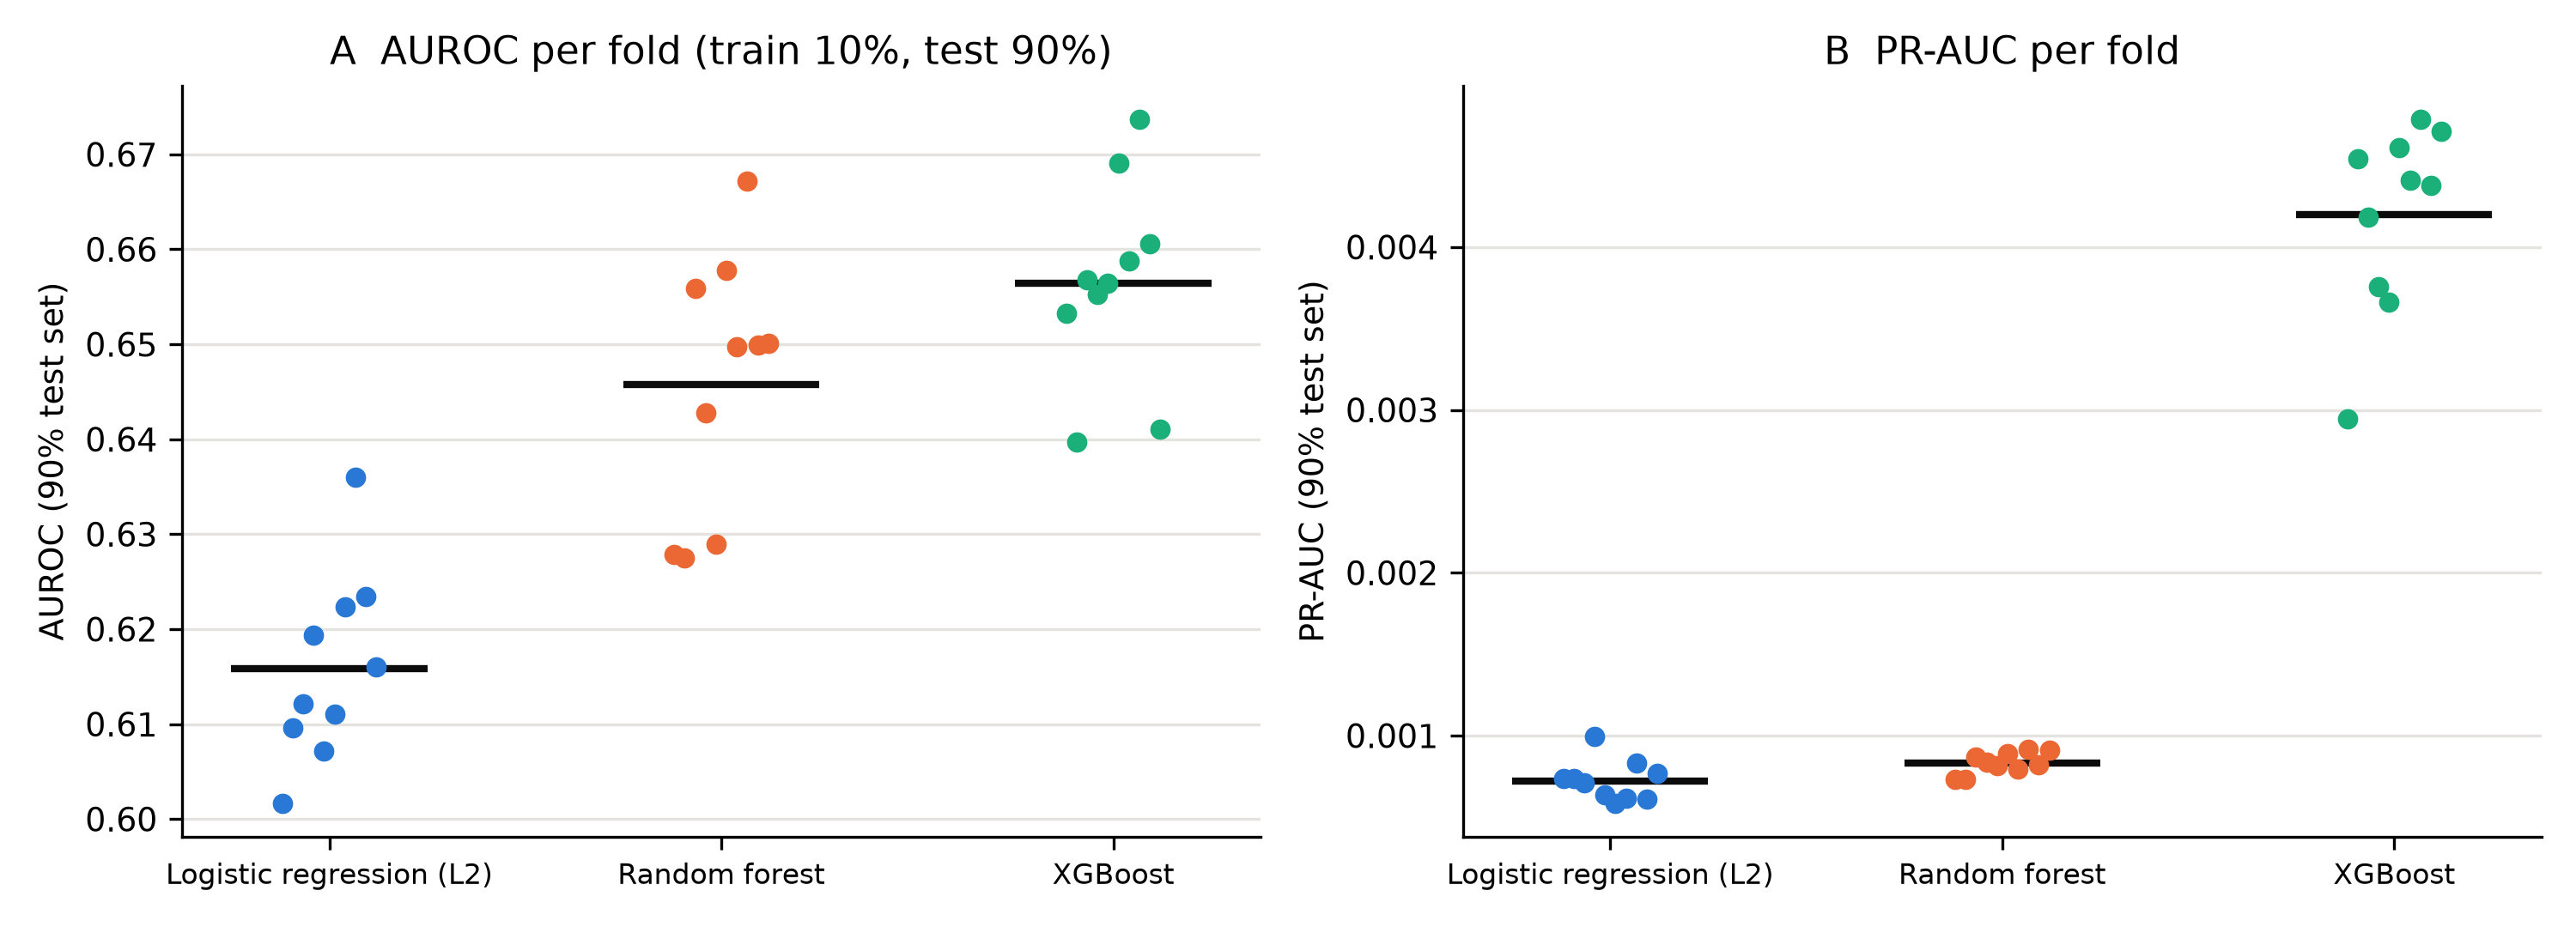
\includegraphics[width=1\linewidth,height=\textheight,keepaspectratio,alt={Performance across ten disjoint 10\% training folds (each tested on the remaining 90\%). (A) AUROC and (B) PR-AUC; each dot is one fold and the horizontal bar is the mean. Blue, logistic regression (L2); orange, random forest; green, XGBoost. PR-AUC values are small because the event rate is 0.044\%. Remaining abbreviations and variable names: Nomenclature appendix.}]{figures/fig_kfold.png}
\caption{Performance across ten disjoint 10\% training folds (each
tested on the remaining 90\%). (A) AUROC and (B) PR-AUC; each dot is one
fold and the horizontal bar is the mean. Blue, logistic regression (L2);
orange, random forest; green, XGBoost. PR-AUC values are small because
the event rate is 0.044\%. Remaining abbreviations and variable names:
Nomenclature appendix.}
\end{figure}

\begin{figure}
\centering
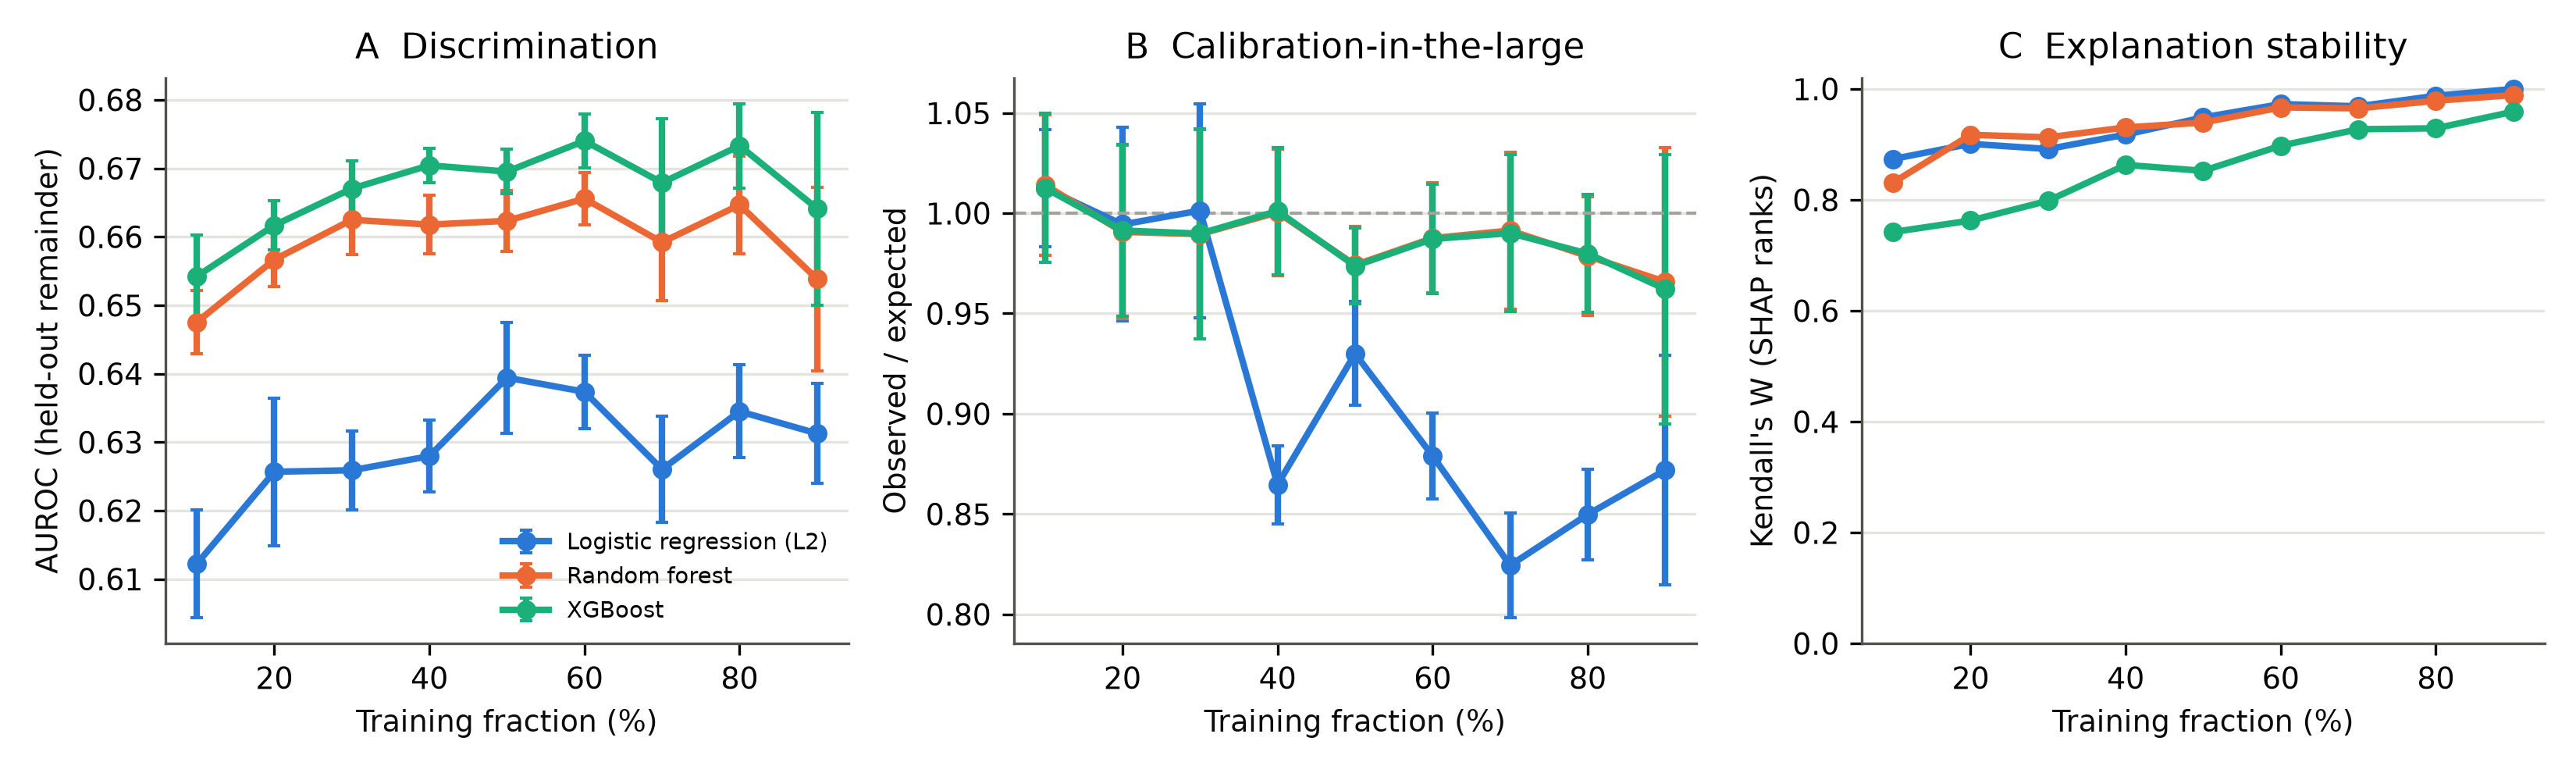
\includegraphics[width=1\linewidth,height=\textheight,keepaspectratio,alt={Training-fraction sweep: models trained on 10\% to 90\% of patients and tested on the remainder (10 repeats per fraction; points = mean, bars = SD). (A) AUROC on the held-out remainder. (B) Calibration-in-the-large as observed/expected (O/E) events; dashed line = 1 (perfect). (C) Stability of explanations: Kendall's W agreement of SHAP feature rankings across repeats (1 = identical rankings). Blue, logistic regression (L2); orange, random forest; green, XGBoost. Remaining abbreviations and variable names: Nomenclature appendix.}]{figures/fig_train_fraction_curves.png}
\caption{Training-fraction sweep: models trained on 10\% to 90\% of
patients and tested on the remainder (10 repeats per fraction; points =
mean, bars = SD). (A) AUROC on the held-out remainder. (B)
Calibration-in-the-large as observed/expected (O/E) events; dashed line
= 1 (perfect). (C) Stability of explanations: Kendall's W agreement of
SHAP feature rankings across repeats (1 = identical rankings). Blue,
logistic regression (L2); orange, random forest; green, XGBoost.
Remaining abbreviations and variable names: Nomenclature appendix.}
\end{figure}

\begin{table}[!htbp]\centering\caption{Training-fraction sweep (mean over 10 repeats). Training fraction =
share of patients used for training; AUROC and AUROC SD = mean and SD of
AUROC on the remainder; PR-AUC = area under the precision-recall curve;
Brier = Brier score; Cal. slope = calibration slope (1 = ideal); O/E and
O/E SD = observed/expected events (1 = ideal). LR, L2 logistic
regression; RF, random forest; XGB, XGBoost. Remaining abbreviations and
variable names: Nomenclature appendix.}\scriptsize
\maxwbox{\textwidth}{\begin{tabular}{lllllllll}\toprule
Model & Training fraction & AUROC & AUROC SD & PR-AUC & Brier & Cal. slope & O/E & O/E SD \\
\midrule
LR & 10\% & 0.6122 & 0.0127 & 0.0007 & 0.0004 & 0.9831 & 1.0125 & 0.0471 \\
LR & 20\% & 0.6257 & 0.0174 & 0.0011 & 0.0004 & 0.9851 & 0.9944 & 0.0779 \\
LR & 30\% & 0.6259 & 0.0093 & 0.001 & 0.0004 & 0.9849 & 1.0013 & 0.0861 \\
LR & 40\% & 0.628 & 0.0085 & 0.0009 & 0.0004 & 1.0021 & 0.8647 & 0.0313 \\
LR & 50\% & 0.6394 & 0.0131 & 0.0008 & 0.0004 & 0.9942 & 0.93 & 0.0418 \\
LR & 60\% & 0.6374 & 0.0087 & 0.0009 & 0.0004 & 1.0002 & 0.879 & 0.0345 \\
LR & 70\% & 0.626 & 0.0125 & 0.0013 & 0.0004 & 1.0084 & 0.8244 & 0.0422 \\
LR & 80\% & 0.6345 & 0.0109 & 0.0015 & 0.0004 & 1.005 & 0.8498 & 0.0365 \\
LR & 90\% & 0.6313 & 0.0118 & 0.0035 & 0.0004 & 1.0018 & 0.8719 & 0.0921 \\
RF & 10\% & 0.6475 & 0.0074 & 0.0008 & 0.0004 & 0.9823 & 1.0141 & 0.0565 \\
RF & 20\% & 0.6567 & 0.0063 & 0.001 & 0.0004 & 0.9864 & 0.9907 & 0.0697 \\
RF & 30\% & 0.6625 & 0.0082 & 0.0009 & 0.0004 & 0.9869 & 0.9895 & 0.0842 \\
RF & 40\% & 0.6618 & 0.0069 & 0.0009 & 0.0004 & 0.9844 & 1.0004 & 0.0509 \\
RF & 50\% & 0.6623 & 0.0071 & 0.0009 & 0.0004 & 0.9877 & 0.9742 & 0.031 \\
RF & 60\% & 0.6656 & 0.0062 & 0.0009 & 0.0004 & 0.9861 & 0.9876 & 0.0443 \\
RF & 70\% & 0.6592 & 0.0137 & 0.0009 & 0.0004 & 0.9856 & 0.9914 & 0.0632 \\
RF & 80\% & 0.6647 & 0.0115 & 0.0009 & 0.0004 & 0.9874 & 0.9786 & 0.048 \\
RF & 90\% & 0.6538 & 0.0217 & 0.0009 & 0.0004 & 0.9891 & 0.9658 & 0.1082 \\
XGB & 10\% & 0.6542 & 0.0097 & 0.0043 & 0.0004 & 0.9792 & 1.0126 & 0.06 \\
XGB & 20\% & 0.6617 & 0.0058 & 0.0044 & 0.0004 & 0.9848 & 0.9914 & 0.069 \\
XGB & 30\% & 0.667 & 0.0066 & 0.0047 & 0.0004 & 0.9864 & 0.9898 & 0.0844 \\
XGB & 40\% & 0.6704 & 0.0041 & 0.0048 & 0.0004 & 0.9833 & 1.0011 & 0.0513 \\
XGB & 50\% & 0.6695 & 0.0053 & 0.0047 & 0.0004 & 0.9873 & 0.9737 & 0.0304 \\
XGB & 60\% & 0.674 & 0.0063 & 0.0054 & 0.0004 & 0.9856 & 0.9872 & 0.0439 \\
XGB & 70\% & 0.6679 & 0.015 & 0.0051 & 0.0004 & 0.9843 & 0.99 & 0.063 \\
XGB & 80\% & 0.6733 & 0.0099 & 0.0053 & 0.0004 & 0.9867 & 0.9799 & 0.0475 \\
XGB & 90\% & 0.6641 & 0.0227 & 0.0053 & 0.0004 & 0.9885 & 0.9621 & 0.1082 \\
\bottomrule\end{tabular}}
\end{table}

\begin{figure}
\centering
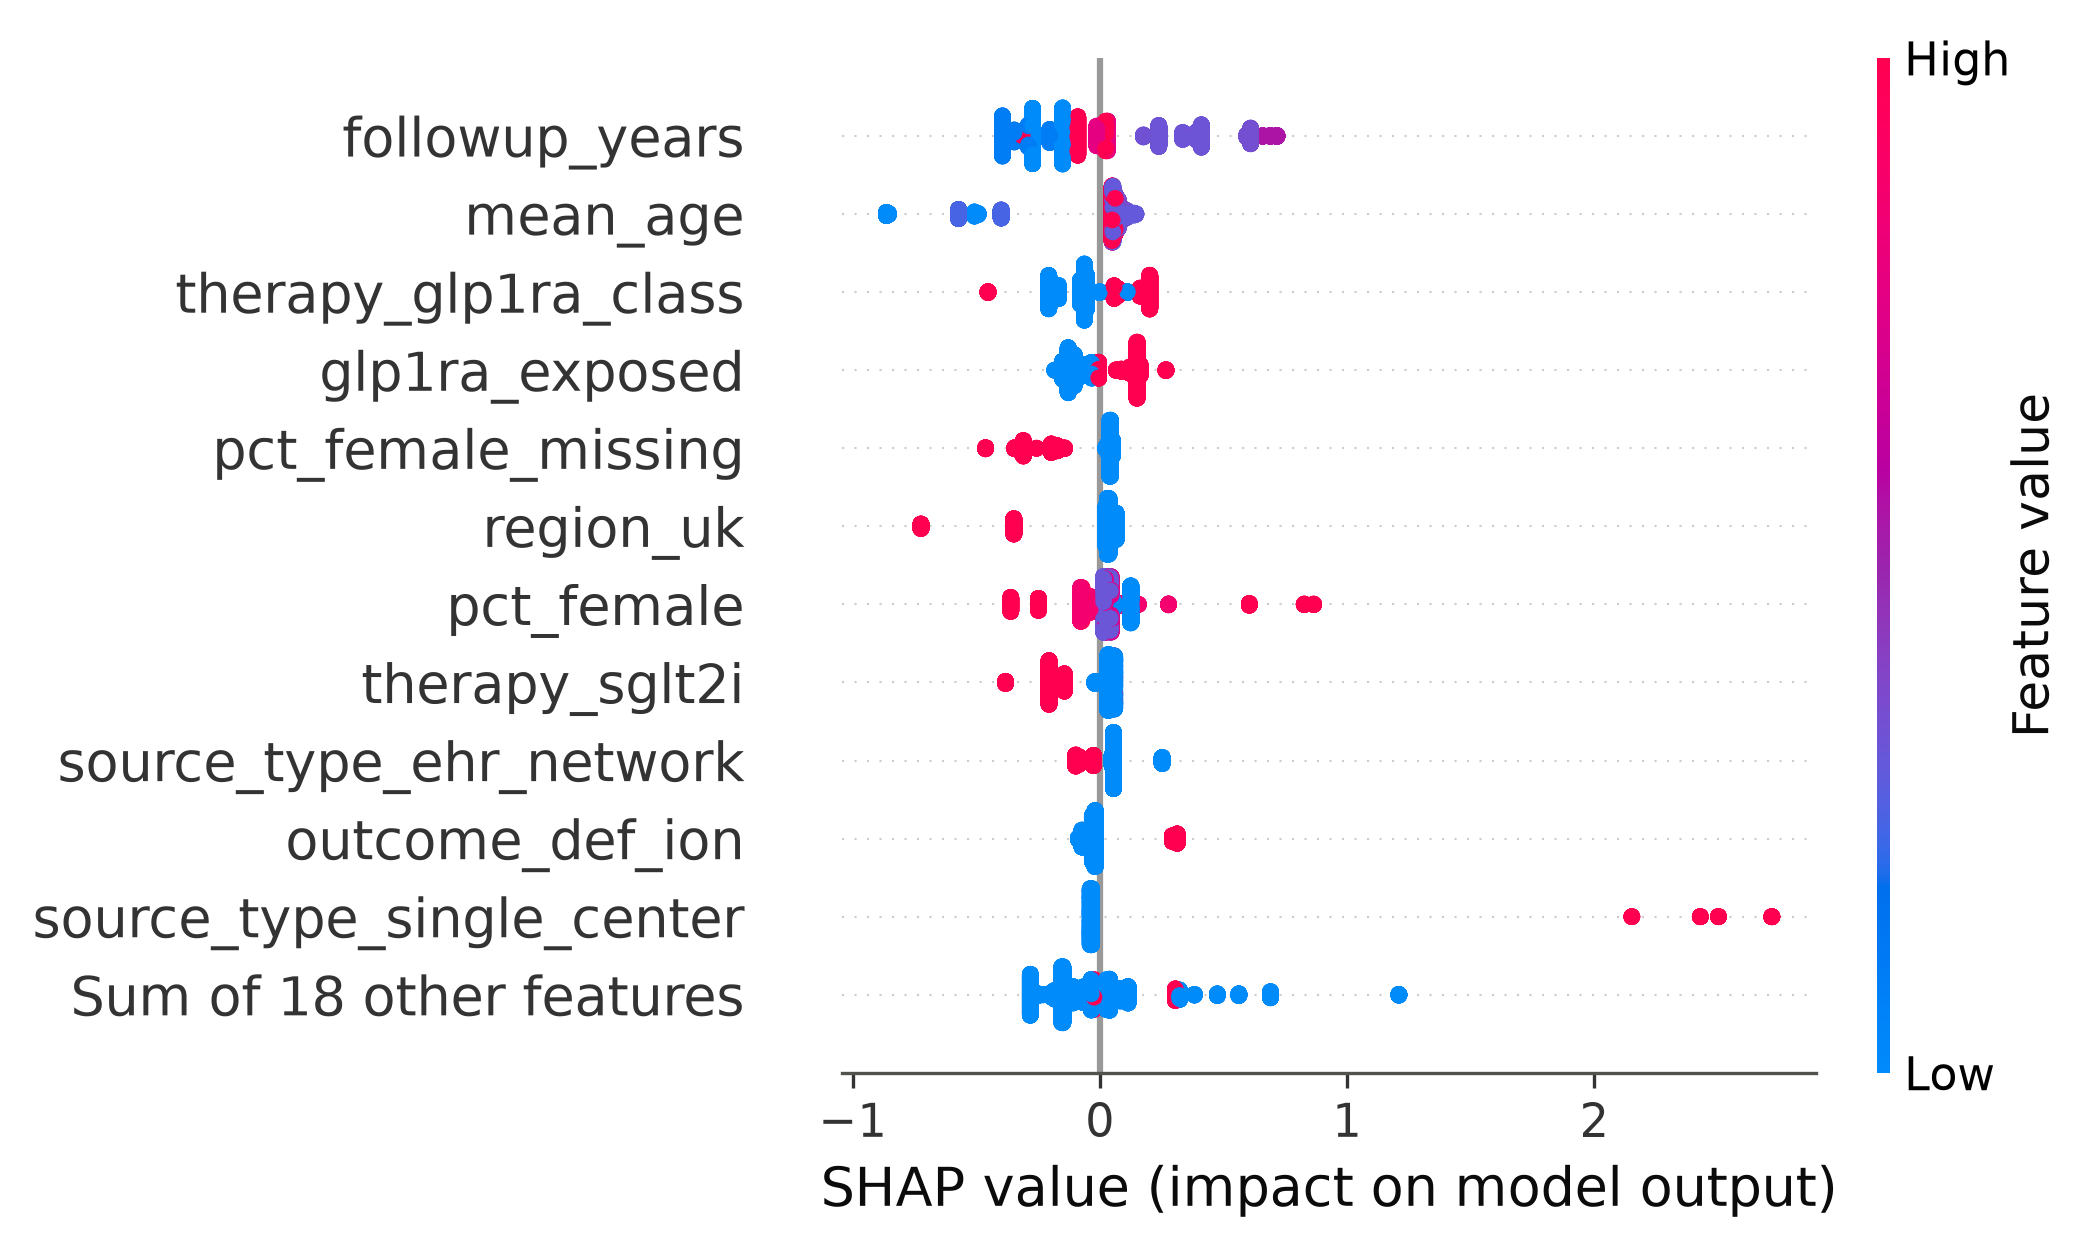
\includegraphics[width=0.85\linewidth,height=\textheight,keepaspectratio,alt={SHAP summary (beeswarm) for XGBoost on the 90\% hold-out. Each dot is one covariate pattern; the x-axis is its SHAP value (contribution to the predicted log-odds of NAION; right = higher risk); colour is the feature value (red = high or 1, blue = low or 0). Features are ordered by mean absolute SHAP value; one-hot features are named variable\_level (e.g., therapy\_sglt2i = SGLT2-inhibitor comparator arm; source\_type\_single\_center = single-center data source). Remaining abbreviations and variable names: Nomenclature appendix.}]{figures/fig_shap_beeswarm_xgb.png}
\caption{SHAP summary (beeswarm) for XGBoost on the 90\% hold-out. Each
dot is one covariate pattern; the x-axis is its SHAP value (contribution
to the predicted log-odds of NAION; right = higher risk); colour is the
feature value (red = high or 1, blue = low or 0). Features are ordered
by mean absolute SHAP value; one-hot features are named variable\_level
(e.g., therapy\_sglt2i = SGLT2-inhibitor comparator arm;
source\_type\_single\_center = single-center data source). Remaining
abbreviations and variable names: Nomenclature appendix.}
\end{figure}

\begin{figure}
\centering
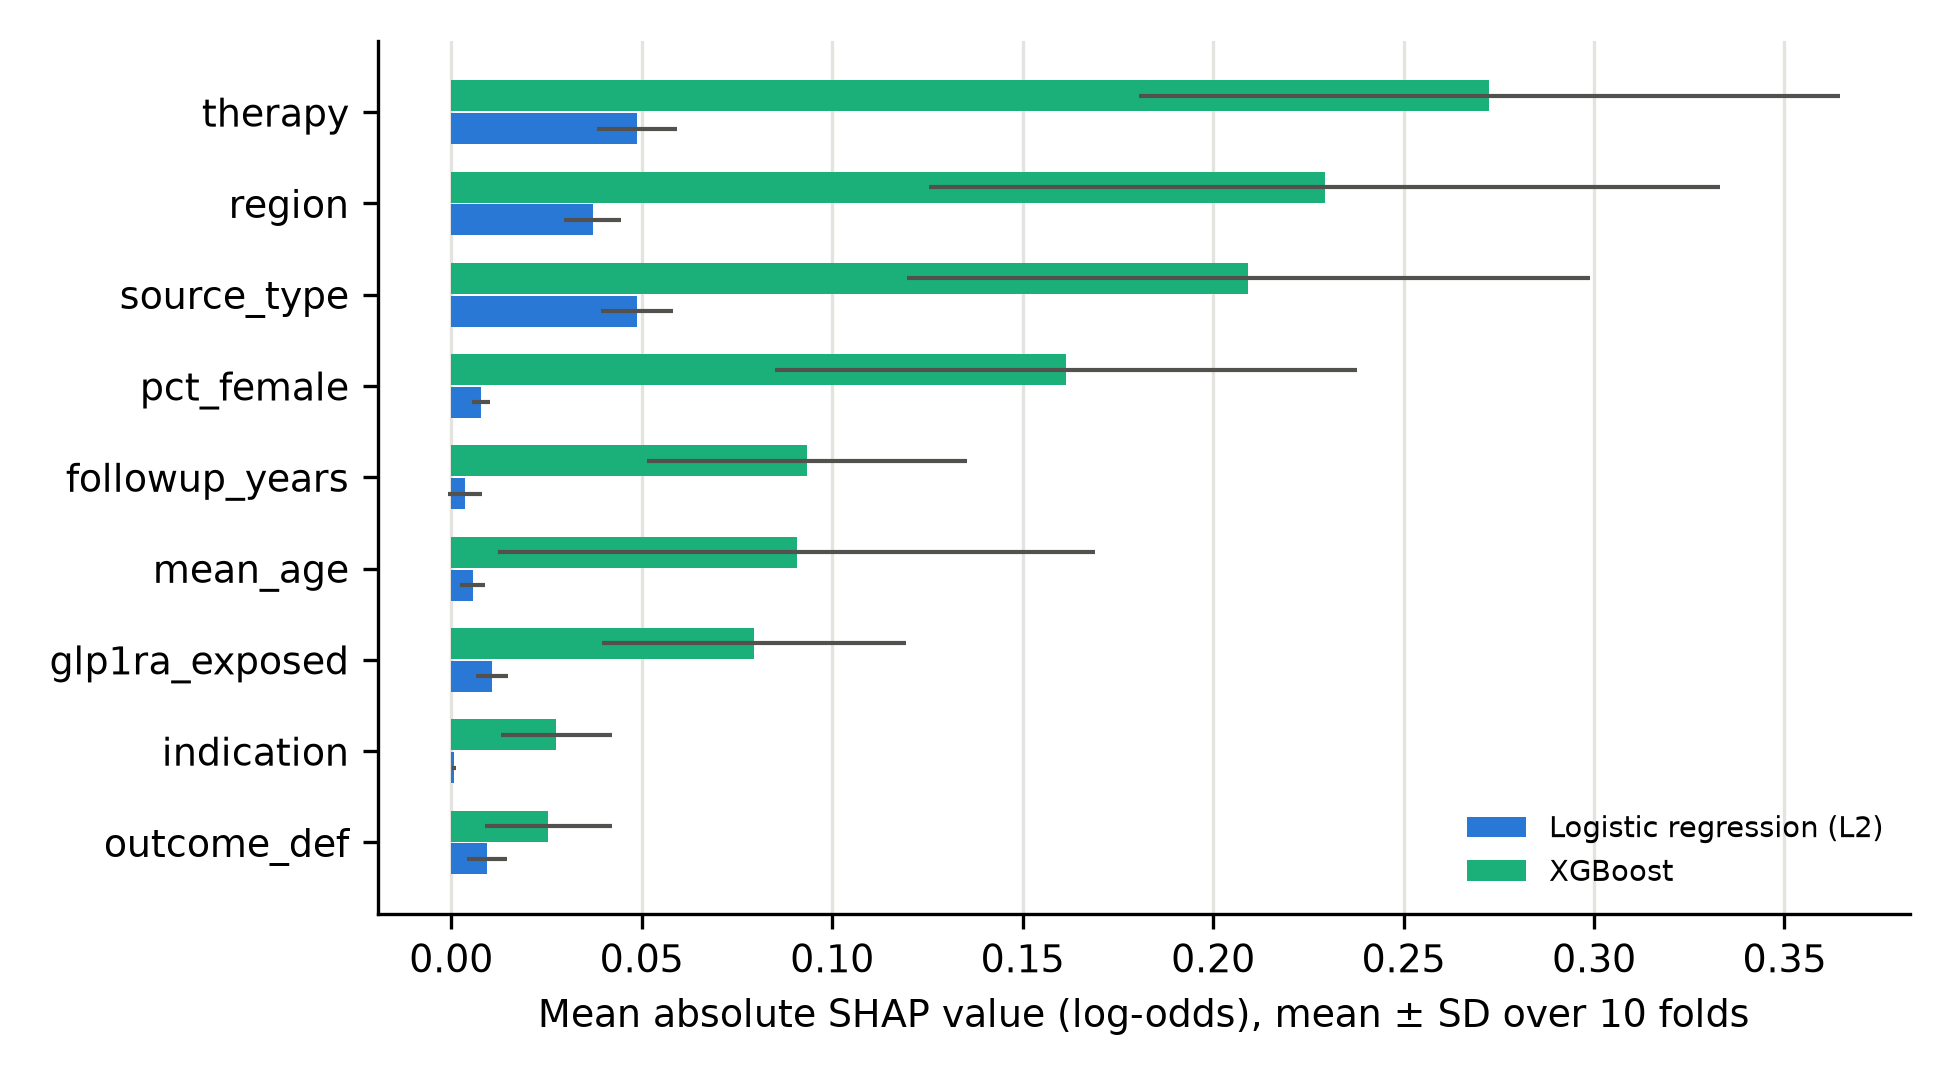
\includegraphics[width=0.85\linewidth,height=\textheight,keepaspectratio,alt={Feature-group importance across ten folds: mean absolute SHAP value (log-odds scale; bars = mean, whiskers = SD over folds), with one-hot levels summed into their parent variable (therapy = drug arm; region; source\_type = data source; outcome\_def = outcome definition). Blue, logistic regression (L2); green, XGBoost; random-forest SHAP values are on the probability scale (about 0.0001) and therefore not shown. Remaining abbreviations and variable names: Nomenclature appendix.}]{figures/fig_shap_kfold_importance.png}
\caption{Feature-group importance across ten folds: mean absolute SHAP
value (log-odds scale; bars = mean, whiskers = SD over folds), with
one-hot levels summed into their parent variable (therapy = drug arm;
region; source\_type = data source; outcome\_def = outcome definition).
Blue, logistic regression (L2); green, XGBoost; random-forest SHAP
values are on the probability scale (about 0.0001) and therefore not
shown. Remaining abbreviations and variable names: Nomenclature
appendix.}
\end{figure}

\section{Statistical inference (all P values, Benjamini-Hochberg q
within
family)}\label{statistical-inference-all-p-values-benjamini-hochberg-q-within-family}

{\footnotesize
\begin{longtable}[]{@{}
  >{\raggedright\arraybackslash}p{(\linewidth - 12\tabcolsep) * \real{0.1879}}
  >{\raggedright\arraybackslash}p{(\linewidth - 12\tabcolsep) * \real{0.4970}}
  >{\raggedright\arraybackslash}p{(\linewidth - 12\tabcolsep) * \real{0.0424}}
  >{\raggedright\arraybackslash}p{(\linewidth - 12\tabcolsep) * \real{0.0848}}
  >{\raggedright\arraybackslash}p{(\linewidth - 12\tabcolsep) * \real{0.0909}}
  >{\raggedright\arraybackslash}p{(\linewidth - 12\tabcolsep) * \real{0.0485}}
  >{\raggedright\arraybackslash}p{(\linewidth - 12\tabcolsep) * \real{0.0485}}@{}}
\caption{Within-study associations with NAION (count-weighted logistic
regression with study fixed effects). Specification = the regression
model in which the term was estimated. Terms: exposed\_ = GLP-1RA
exposure in the named drug or indication subgroup; exposed\_vs\_ =
versus the named comparator; exposed\_x\_ = interaction with the named
study-level covariate (per 10 years of mean age, per 10 percentage
points of women, per year of follow-up). OR = odds ratio; q =
Benjamini-Hochberg adjusted P value. Remaining abbreviations and
variable names: Nomenclature appendix.}\tabularnewline
\toprule\noalign{}
\begin{minipage}[b]{\linewidth}\raggedright
Term
\end{minipage} & \begin{minipage}[b]{\linewidth}\raggedright
Specification
\end{minipage} & \begin{minipage}[b]{\linewidth}\raggedright
OR
\end{minipage} & \begin{minipage}[b]{\linewidth}\raggedright
95\% CI low
\end{minipage} & \begin{minipage}[b]{\linewidth}\raggedright
95\% CI high
\end{minipage} & \begin{minipage}[b]{\linewidth}\raggedright
P
\end{minipage} & \begin{minipage}[b]{\linewidth}\raggedright
q
\end{minipage} \\
\midrule\noalign{}
\endfirsthead
\toprule\noalign{}
\begin{minipage}[b]{\linewidth}\raggedright
Term
\end{minipage} & \begin{minipage}[b]{\linewidth}\raggedright
Specification
\end{minipage} & \begin{minipage}[b]{\linewidth}\raggedright
OR
\end{minipage} & \begin{minipage}[b]{\linewidth}\raggedright
95\% CI low
\end{minipage} & \begin{minipage}[b]{\linewidth}\raggedright
95\% CI high
\end{minipage} & \begin{minipage}[b]{\linewidth}\raggedright
P
\end{minipage} & \begin{minipage}[b]{\linewidth}\raggedright
q
\end{minipage} \\
\midrule\noalign{}
\endhead
\bottomrule\noalign{}
\endlastfoot
glp1ra\_exposed & A2 study fixed effects: any GLP-1RA vs comparator &
1.587 & 1.422 & 1.772 & \textless0.001 & \textless0.001 \\
exposed\_semaglutide & A2 study FE: exposure by drug & 1.730 & 1.439 &
2.080 & \textless0.001 & \textless0.001 \\
exposed\_glp1ra\_class & A2 study FE: exposure by drug & 1.496 & 1.300 &
1.721 & \textless0.001 & \textless0.001 \\
exposed\_sema\_or\_tirz & A2 study FE: exposure by drug & 1.842 & 1.054
& 3.221 & 0.032 & 0.044 \\
exposed\_t2d & A2 study FE: exposure by indication & 1.622 & 1.448 &
1.817 & \textless0.001 & \textless0.001 \\
exposed\_obesity & A2 study FE: exposure by indication & 2.697 & 1.637 &
4.441 & \textless0.001 & \textless0.001 \\
exposed\_iih & A2 study FE: exposure by indication & 0.428 & 0.218 &
0.842 & 0.014 & 0.021 \\
exposed\_vs\_dpp4i & A2 study FE: exposure by comparator class & 1.029 &
0.571 & 1.855 & 0.924 & 0.943 \\
exposed\_vs\_no\_glp1ra & A2 study FE: exposure by comparator class &
1.143 & 0.936 & 1.394 & 0.189 & 0.236 \\
exposed\_vs\_other\_antidiabetic & A2 study FE: exposure by comparator
class & 2.348 & 1.743 & 3.164 & \textless0.001 & \textless0.001 \\
exposed\_vs\_sglt2i & A2 study FE: exposure by comparator class & 1.806
& 1.544 & 2.113 & \textless0.001 & \textless0.001 \\
glp1ra\_exposed & A2 study FE: exposure effect modification (study-level
age, \% female, follow-up) & 1.411 & 1.244 & 1.602 & \textless0.001 &
\textless0.001 \\
exposed\_x\_age\_per\_10y & A2 study FE: exposure effect modification
(study-level age, \% female, follow-up) & 1.989 & 1.301 & 3.041 & 0.001
& 0.002 \\
exposed\_x\_female\_per\_10pct & A2 study FE: exposure effect
modification (study-level age, \% female, follow-up) & 0.996 & 0.886 &
1.120 & 0.943 & 0.943 \\
exposed\_x\_followup\_years & A2 study FE: exposure effect modification
(study-level age, \% female, follow-up) & 1.021 & 0.945 & 1.103 & 0.595
& 0.687 \\
\end{longtable}
}

\begin{table}[!htbp]\centering\caption{Marginal associations with NAION across studies (count-weighted logistic
regression with cluster-robust standard errors by study). These
comparisons are ecological and confounded by study setting. Feature
names: therapy\_, indication\_, region\_, source\_type\_, outcome\_def\_
= one-hot levels (reference levels omitted); OR = odds ratio; q =
Benjamini-Hochberg adjusted P value. Remaining abbreviations and
variable names: Nomenclature appendix.}\scriptsize
\maxwbox{\textwidth}{\begin{tabular}{llllll}\toprule
Term & OR & 95\% CI low & 95\% CI high & P & q \\
\midrule
therapy\_dpp4i & 1.055 & 0.712 & 1.564 & 0.789 & 0.789 \\
therapy\_glp1ra\_class & 1.086 & 0.733 & 1.610 & 0.681 & 0.766 \\
therapy\_other\_antidiabetic & 0.628 & 0.342 & 1.154 & 0.134 & 0.201 \\
therapy\_other\_antiobesity & 0.123 & 0.096 & 0.156 & \textless0.001 & \textless0.001 \\
therapy\_sema\_or\_tirz & 1.158 & 0.630 & 2.127 & 0.637 & 0.764 \\
therapy\_semaglutide & 1.215 & 0.954 & 1.547 & 0.114 & 0.187 \\
therapy\_sglt2i & 0.614 & 0.424 & 0.890 & 0.010 & 0.023 \\
indication\_iih & 86.796 & 1.014 & 7429.090 & 0.049 & 0.089 \\
indication\_obesity & 0.630 & 0.402 & 0.985 & 0.043 & 0.086 \\
region\_nordic & 1.951 & 1.520 & 2.506 & \textless0.001 & \textless0.001 \\
region\_uk & 0.213 & 0.182 & 0.250 & \textless0.001 & \textless0.001 \\
source\_type\_claims & 0.540 & 0.180 & 1.627 & 0.274 & 0.379 \\
source\_type\_single\_center & 326.045 & 217.289 & 489.235 & \textless0.001 & \textless0.001 \\
source\_type\_va\_ehr & 0.551 & 0.090 & 3.385 & 0.520 & 0.669 \\
outcome\_def\_ion & 0.494 & 0.415 & 0.587 & \textless0.001 & \textless0.001 \\
age\_per\_10y & 1.538 & 0.098 & 24.122 & 0.759 & 0.789 \\
female\_per\_10pct & 0.499 & 0.301 & 0.828 & 0.007 & 0.018 \\
followup\_years & 0.756 & 0.697 & 0.820 & \textless0.001 & \textless0.001 \\
\bottomrule\end{tabular}}
\end{table}

\begin{table}[!htbp]\centering\caption{SHAP permutation tests (B = 500 permutations). Mean abs. SHAP = mean
absolute SHAP value (XGBoost, log-odds); P (global null) = outcome
permuted across all patients; P (within-study null) = outcome permuted
within studies, which tests whether the feature carries information
beyond study membership; q = Benjamini-Hochberg adjusted P value.
Remaining abbreviations and variable names: Nomenclature appendix.}\scriptsize
\maxwbox{\textwidth}{\begin{tabular}{lllll}\toprule
Feature & Mean abs. SHAP & P (global null) & q & P (within-study null) \\
\midrule
followup\_years & 0.031 & 0.186 & 0.209 & 0.996 \\
glp1ra\_exposed & 0.118 & 0.002 & 0.004 & 0.002 \\
indication & 0.015 & 0.008 & 0.014 & 1.000 \\
mean\_age & 0.057 & 0.026 & 0.033 & 0.255 \\
outcome\_def & 0.011 & 0.228 & 0.228 & 0.030 \\
pct\_female & 0.112 & 0.002 & 0.004 & 0.146 \\
region & 0.263 & 0.002 & 0.004 & 0.369 \\
source\_type & 0.143 & 0.002 & 0.004 & 0.916 \\
therapy & 0.141 & 0.010 & 0.015 & 0.012 \\
\bottomrule\end{tabular}}
\end{table}

\begin{table}[!htbp]\centering\caption{Random-effects (DerSimonian-Laird) meta-analysis of published ratio
estimates. k = number of estimates; I2 = percentage of variance due to
between-study heterogeneity; q = Benjamini-Hochberg adjusted P value.
Remaining abbreviations and variable names: Nomenclature appendix.}\scriptsize
\maxwbox{\textwidth}{\begin{tabular}{llllllll}\toprule
Analysis & k & Pooled ratio & 95\% CI low & 95\% CI high & I2 & P & q \\
\midrule
All studies (most precise estimate each) & 25.000 & 1.341 & 1.161 & 1.549 & 86.6 & \textless0.001 & \textless0.001 \\
Indication = T2D & 20.000 & 1.363 & 1.163 & 1.598 & 87.8 & \textless0.001 & \textless0.001 \\
Indication = T2D or obesity & 2.000 & 1.859 & 0.764 & 4.525 & 86.9 & 0.172 & 0.229 \\
Subgroup difference by indication & 2.000 & --- & --- & --- & --- & 0.501 & 0.501 \\
Drug = any GLP-1RA & 15.000 & 1.302 & 1.128 & 1.504 & 81.1 & \textless0.001 & \textless0.001 \\
Drug = semaglutide & 8.000 & 1.569 & 1.007 & 2.444 & 91.9 & 0.047 & 0.075 \\
Subgroup difference by drug & 2.000 & --- & --- & --- & --- & 0.434 & 0.496 \\
Excluding IIH cohort & 24.000 & 1.380 & 1.196 & 1.592 & 86.4 & \textless0.001 & \textless0.001 \\
\bottomrule\end{tabular}}
\end{table}

\begin{table}[!htbp]\centering\caption{Demographic contrasts: observed versus expected values (e.g., share of
men among case reports versus exposed cohorts) with the stated test; q =
Benjamini-Hochberg adjusted P value. Remaining abbreviations and
variable names: Nomenclature appendix.}\scriptsize
\maxwbox{\textwidth}{\begin{tabular}{llllll}\toprule
Contrast & Observed & Expected & Test & P & q \\
\midrule
case reports: male share vs exposed-cohort male share & 0.688 & 0.490 & exact binomial & 0.137 & 0.274 \\
case reports: age vs exposed-cohort mean age & 47.000 & 60.150 & Wilcoxon signed-rank vs cohort mean & 0.003 & 0.016 \\
case reports: obesity indication share vs 50\% & 0.786 & 0.500 & exact binomial & 0.057 & 0.172 \\
meta-analysis 42612051: age \textless65 vs \textgreater=65 & 2.187 & 1.000 & z-test of ratio of ratios (from published CIs) & 0.272 & 0.407 \\
meta-analysis 42612051: female- vs male-dominant cohorts & 0.951 & 1.000 & z-test of ratio of ratios (from published CIs) & 0.919 & 0.919 \\
meta-analysis 42612051: diabetes vs obesity indication & 1.095 & 1.000 & z-test of ratio of ratios (from published CIs) & 0.850 & 0.919 \\
\bottomrule\end{tabular}}
\end{table}

\begin{table}[!htbp]\centering\caption{Statistical tests of the machine-learning experiments. Estimate = the
tested quantity (AUROC, difference or rank correlation); Hanley-McNeil =
AUROC standard error; Nadeau-Bengio corrected = resampled t test
corrected for overlapping training sets; Wilcoxon and Spearman as
stated; q = Benjamini-Hochberg adjusted P value. Remaining abbreviations
and variable names: Nomenclature appendix.}\scriptsize
\maxwbox{\textwidth}{\begin{tabular}{lllll}\toprule
Experiment & Estimate & Test & P & q \\
\midrule
LR: AUROC \textgreater{} 0.5 (10/90 hold-out) & 0.627 & Hanley-McNeil one-sided & \textless0.001 & \textless0.001 \\
RF: AUROC \textgreater{} 0.5 (10/90 hold-out) & 0.642 & Hanley-McNeil one-sided & \textless0.001 & \textless0.001 \\
XGB: AUROC \textgreater{} 0.5 (10/90 hold-out) & 0.657 & Hanley-McNeil one-sided & \textless0.001 & \textless0.001 \\
XGB vs LR: AUROC difference (10 x 10\% folds) & 0.041 & Nadeau-Bengio corrected resampled t & 0.218 & 0.277 \\
XGB vs RF: AUROC difference (10 x 10\% folds) & 0.011 & Nadeau-Bengio corrected resampled t & 0.745 & 0.745 \\
RF vs LR: AUROC difference (10 x 10\% folds) & 0.030 & Nadeau-Bengio corrected resampled t & 0.314 & 0.339 \\
LR: leave-one-study-out AUROC \textgreater{} 0.5 & 0.510 & Wilcoxon over 11 held-out studies & 0.289 & 0.337 \\
RF: leave-one-study-out AUROC \textgreater{} 0.5 & 0.532 & Wilcoxon over 11 held-out studies & 0.087 & 0.136 \\
XGB: leave-one-study-out AUROC \textgreater{} 0.5 & 0.535 & Wilcoxon over 11 held-out studies & 0.021 & 0.037 \\
LR: AUROC trend with training fraction (10-90\%) & 0.304 & Spearman (90 runs) & 0.004 & 0.008 \\
RF: AUROC trend with training fraction (10-90\%) & 0.266 & Spearman (90 runs) & 0.011 & 0.023 \\
XGB: AUROC trend with training fraction (10-90\%) & 0.389 & Spearman (90 runs) & \textless0.001 & \textless0.001 \\
Stage 2 hybrid best vs PubMed-only (XGB, paired) & 0.001 & paired z over 27 split/seed pairs & 0.167 & 0.233 \\
Stage 2 synthetic-only best vs PubMed-only (XGB, paired) & -0.010 & paired z over 27 split/seed pairs & \textless0.001 & \textless0.001 \\
\bottomrule\end{tabular}}
\end{table}

\begin{figure}
\centering
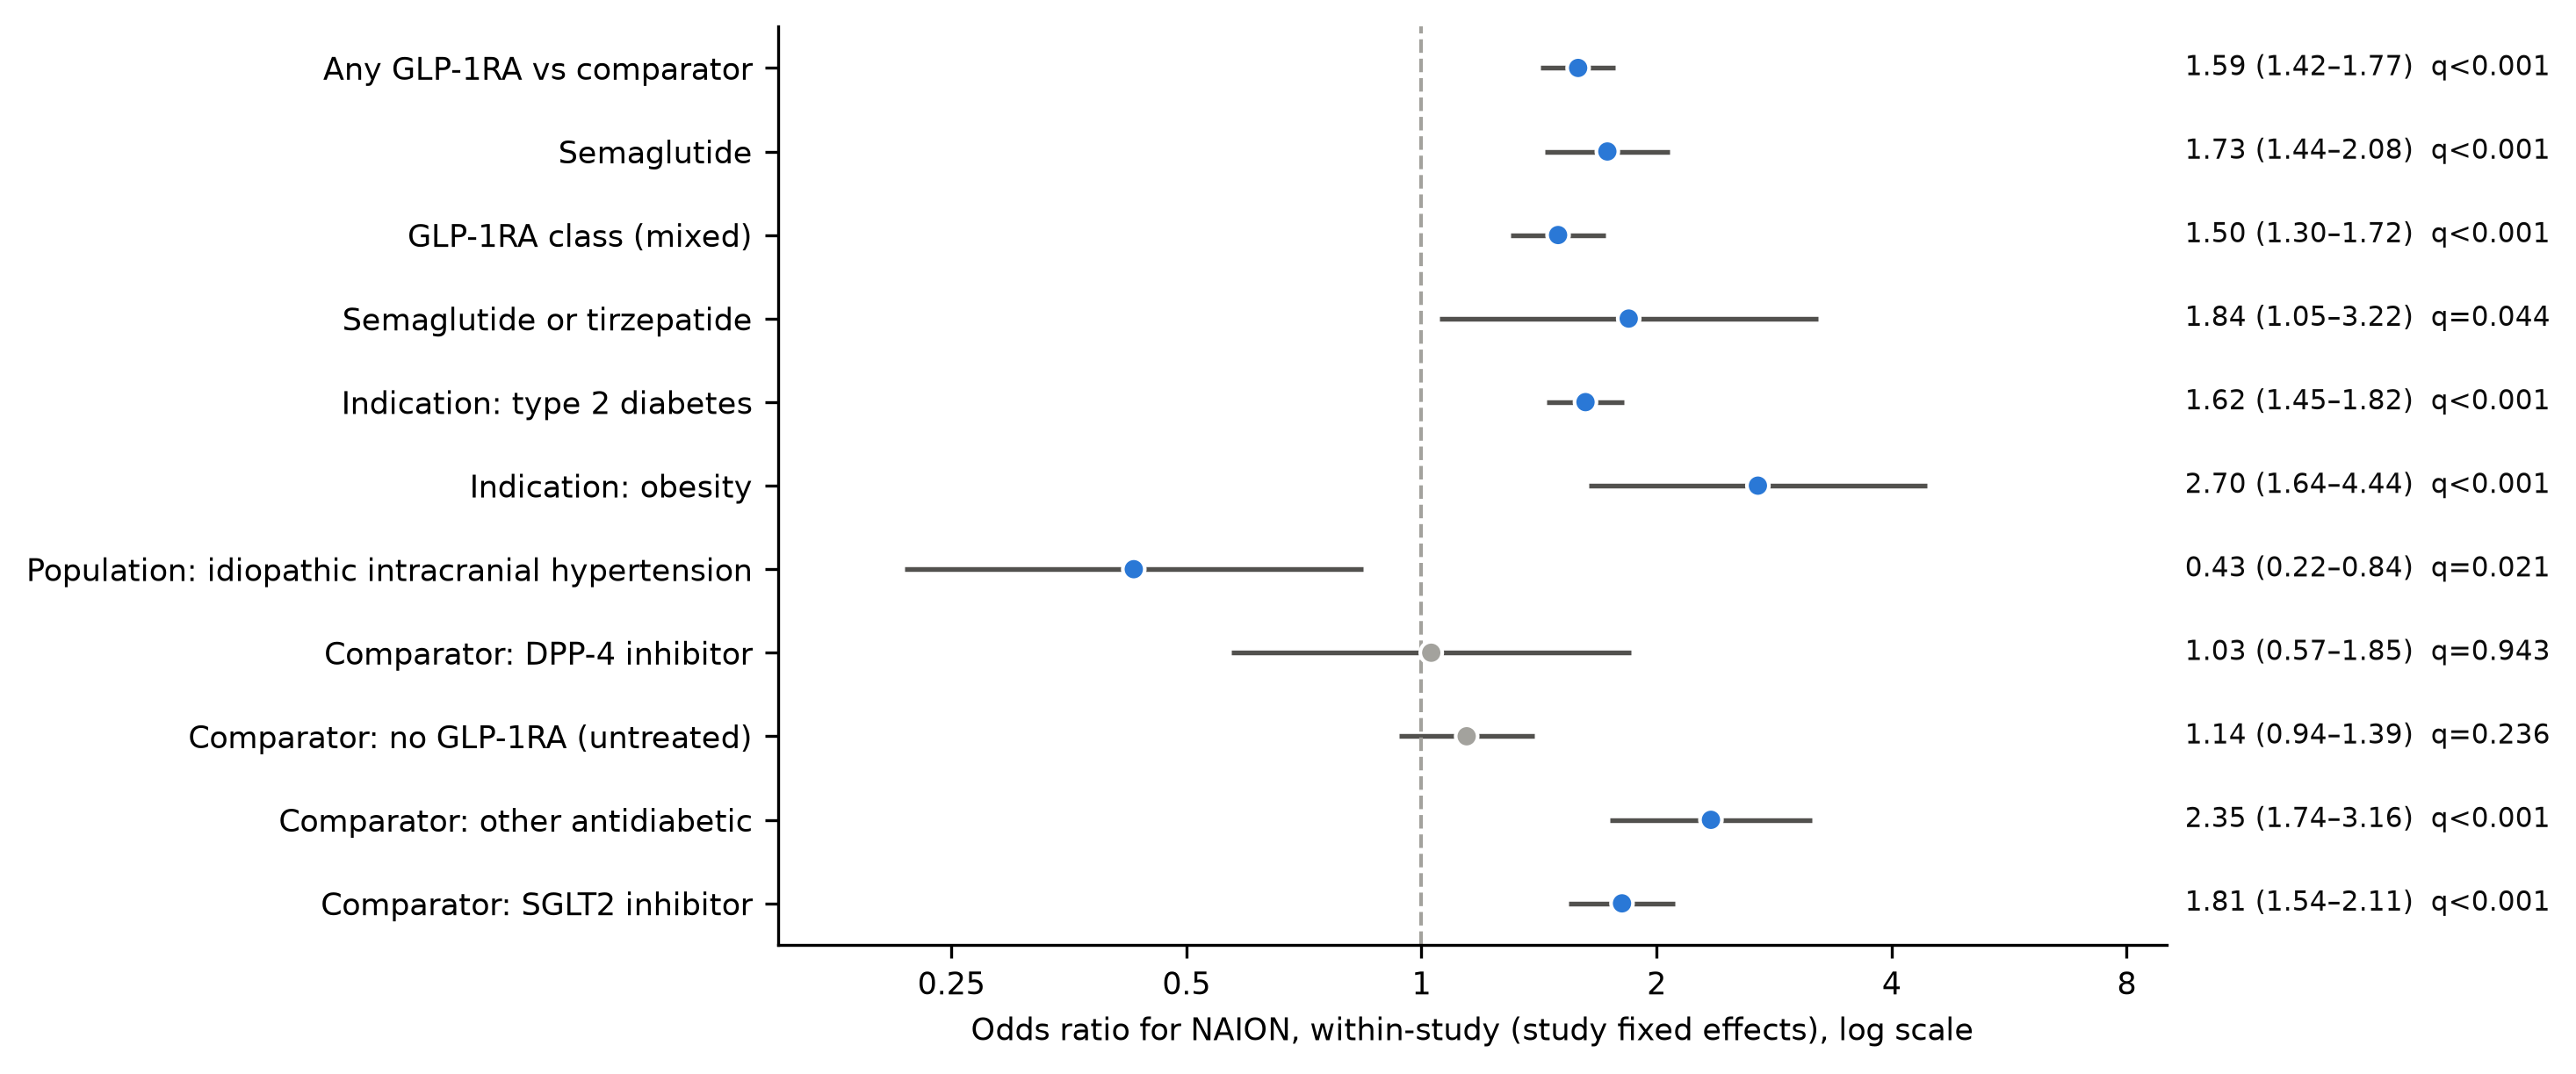
\includegraphics[width=1\linewidth,height=\textheight,keepaspectratio,alt={Within-study odds ratios for NAION (count-weighted logistic regression with study fixed effects, so each estimate compares patients within the same study). Points = odds ratio, lines = 95\% CI, log scale; dashed line = no association. Blue, q \textless{} 0.05; grey, not significant; q = Benjamini-Hochberg adjusted P value. Values at right: OR (95\% CI) and q. Remaining abbreviations and variable names: Nomenclature appendix.}]{figures/fig_forest_within_study.png}
\caption{Within-study odds ratios for NAION (count-weighted logistic
regression with study fixed effects, so each estimate compares patients
within the same study). Points = odds ratio, lines = 95\% CI, log scale;
dashed line = no association. Blue, q \textless{} 0.05; grey, not
significant; q = Benjamini-Hochberg adjusted P value. Values at right:
OR (95\% CI) and q. Remaining abbreviations and variable names:
Nomenclature appendix.}
\end{figure}

\begin{figure}
\centering
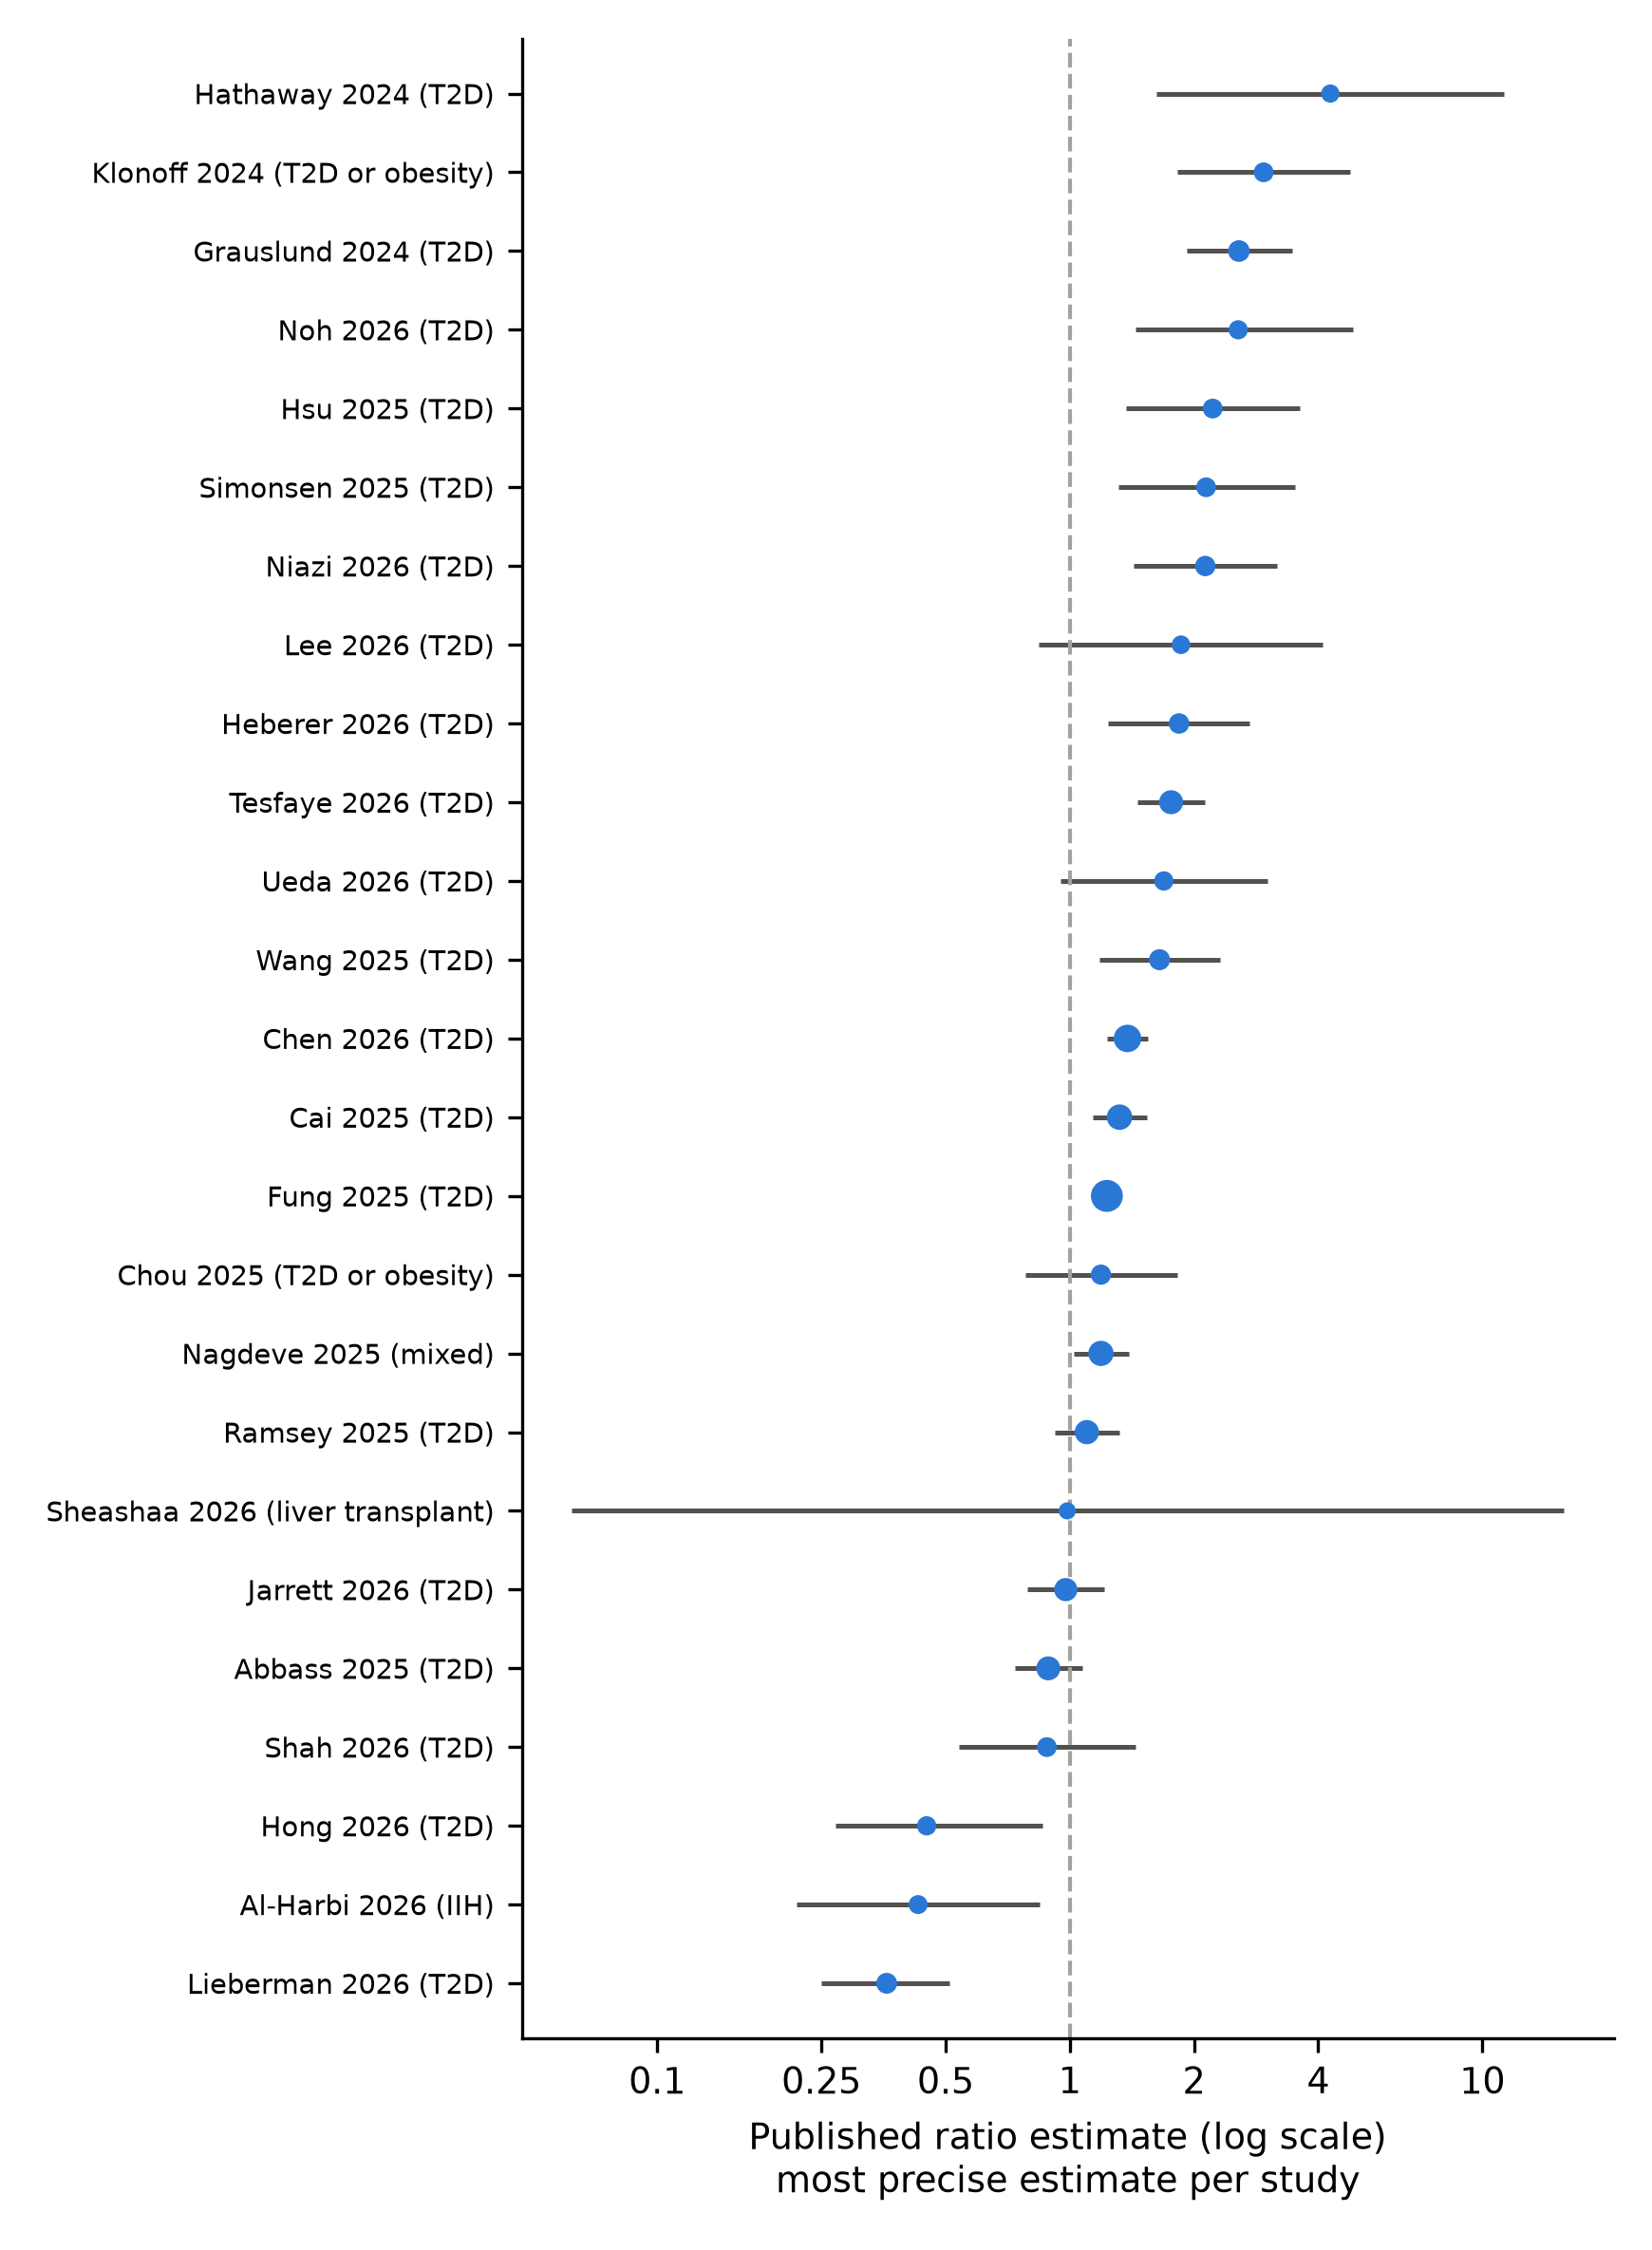
\includegraphics[width=0.8\linewidth,height=\textheight,keepaspectratio,alt={Most precise published ratio estimate per study (smallest standard error), as reported by the authors (hazard, odds, risk or incidence rate ratios; not directly interchangeable). Points = estimate (size proportional to precision), lines = 95\% CI, log scale; dashed line = 1. Labels: first author, year (population). T2D, type 2 diabetes; IIH, idiopathic intracranial hypertension. Remaining abbreviations and variable names: Nomenclature appendix.}]{figures/fig_forest.png}
\caption{Most precise published ratio estimate per study (smallest
standard error), as reported by the authors (hazard, odds, risk or
incidence rate ratios; not directly interchangeable). Points = estimate
(size proportional to precision), lines = 95\% CI, log scale; dashed
line = 1. Labels: first author, year (population). T2D, type 2 diabetes;
IIH, idiopathic intracranial hypertension. Remaining abbreviations and
variable names: Nomenclature appendix.}\label{fig:forestpub}
\end{figure}

\section{Threshold metrics (hold-out; P values against
chance)}\label{threshold-metrics-hold-out-p-values-against-chance}

\begin{table}[!htbp]\centering\caption{Threshold metrics on the 90\% hold-out with P values against chance.
Thresholds: Youden = maximizes sensitivity + specificity - 1; Top 10\% /
Top 20\% = flags the top 10\% or 20\% of training risk. Sens,
sensitivity; Spec, specificity; Acc, accuracy; P (Sens) and P (Spec) =
versus chance; P vs NIR = accuracy versus the no-information rate; P
(NPV) = NPV versus 1 - prevalence; PPV versus prevalence (P vs prev);
NPV, negative predictive value; LR+, positive likelihood ratio; NB, net
benefit at the threshold probability; NB treat-all, net benefit of
treating everyone. Remaining abbreviations and variable names:
Nomenclature appendix.}\scriptsize
\maxwbox{\textwidth}{\begin{tabular}{llllllllllllllll}\toprule
Model & Threshold & AUROC & Sens & P (Sens) & Spec & P (Spec) & Acc & P vs NIR & PPV & P vs prev & NPV & P (NPV) & LR+ & NB & NB treat-all \\
\midrule
LR & Youden & 0.6275 & 0.8080 & \textless0.001 & 0.3958 & 0.377 & 0.3960 & 1.000 & 5.87e-04 & \textless0.001 & 0.9998 & \textless0.001 & 1.3373 & 9.97e-05 & 1.70e-05 \\
LR & Top 10\% & 0.6275 & 0.2167 & \textless0.001 & 0.8697 & 0.424 & 0.8694 & 1.000 & 7.30e-04 & \textless0.001 & 0.9996 & \textless0.001 & 1.6631 & 3.73e-05 & -4.75e-06 \\
LR & Top 20\% & 0.6275 & 0.3769 & \textless0.001 & 0.7640 & 0.402 & 0.7638 & 1.000 & 7.01e-04 & \textless0.001 & 0.9996 & \textless0.001 & 1.5969 & 6.19e-05 & 3.39e-07 \\
RF & Youden & 0.6421 & 0.7190 & \textless0.001 & 0.5107 & 0.365 & 0.5108 & 1.000 & 6.45e-04 & \textless0.001 & 0.9998 & \textless0.001 & 1.4694 & 9.86e-05 & -4.56e-06 \\
RF & Top 10\% & 0.6421 & 0.2051 & \textless0.001 & 0.9309 & 0.344 & 0.9305 & 1.000 & 0.0013 & \textless0.001 & 0.9996 & \textless0.001 & 2.9667 & 5.04e-05 & -1.34e-04 \\
RF & Top 20\% & 0.6421 & 0.3444 & \textless0.001 & 0.7934 & 0.399 & 0.7932 & 1.000 & 7.31e-04 & \textless0.001 & 0.9996 & \textless0.001 & 1.6674 & 4.17e-05 & -9.08e-05 \\
XGB & Youden & 0.6569 & 0.7190 & \textless0.001 & 0.5107 & 0.365 & 0.5108 & 1.000 & 6.45e-04 & \textless0.001 & 0.9998 & \textless0.001 & 1.4694 & 1.08e-04 & 1.51e-05 \\
XGB & Top 10\% & 0.6569 & 0.3235 & \textless0.001 & 0.8500 & 0.358 & 0.8498 & 1.000 & 9.46e-04 & \textless0.001 & 0.9997 & \textless0.001 & 2.1572 & 4.31e-05 & -2.20e-04 \\
XGB & Top 20\% & 0.6569 & 0.3754 & \textless0.001 & 0.7935 & 0.377 & 0.7933 & 1.000 & 7.97e-04 & \textless0.001 & 0.9997 & \textless0.001 & 1.8177 & 3.53e-05 & -1.88e-04 \\
Ensemble & Youden & 0.6568 & 0.7190 & \textless0.001 & 0.5107 & 0.365 & 0.5108 & 1.000 & 6.45e-04 & \textless0.001 & 0.9998 & \textless0.001 & 1.4694 & 9.73e-05 & -7.17e-06 \\
Ensemble & Top 10\% & 0.6568 & 0.3289 & \textless0.001 & 0.8449 & 0.359 & 0.8446 & 1.000 & 9.30e-04 & \textless0.001 & 0.9997 & \textless0.001 & 2.1204 & 5.77e-05 & -1.20e-04 \\
Ensemble & Top 20\% & 0.6568 & 0.3808 & \textless0.001 & 0.7883 & 0.378 & 0.7881 & 1.000 & 7.89e-04 & \textless0.001 & 0.9997 & \textless0.001 & 1.7990 & 5.49e-05 & -9.12e-05 \\
\bottomrule\end{tabular}}
\end{table}

\begin{table}[!htbp]\centering\caption{Threshold metrics across ten folds (mean). Thresholds: Youden =
maximizes Youden's J; Top 10\% and Top 20\% = flag the top 10\% or 20\%
of training risk. All values are means over folds; Sens, sensitivity;
Spec, specificity; Acc, accuracy; LR+, positive likelihood ratio;
Flagged = share of patients flagged. LR, logistic regression; RF, random
forest; XGB, XGBoost; Ensemble = mean of members. Remaining
abbreviations and variable names: Nomenclature appendix.}\scriptsize
\maxwbox{\textwidth}{\begin{tabular}{llllllllll}\toprule
Model & Threshold & AUROC & Sens & Spec & Acc & PPV & NPV & LR+ & Flagged \\
\midrule
Ensemble & Youden & 0.65561 & 0.57248 & 0.62969 & 0.62967 & 0.00069 & 0.99971 & 1.57919 & 0.3704 \\
Ensemble & Top 10\% & 0.65561 & 0.31414 & 0.85511 & 0.85487 & 0.00101 & 0.99965 & 2.31932 & 0.14497 \\
Ensemble & Top 20\% & 0.65561 & 0.42501 & 0.76448 & 0.76433 & 0.0008 & 0.99967 & 1.82865 & 0.2356 \\
LR & Youden & 0.61586 & 0.55674 & 0.61235 & 0.61233 & 0.00064 & 0.99969 & 1.47306 & 0.38772 \\
LR & Top 10\% & 0.61586 & 0.25847 & 0.8481 & 0.84784 & 0.00075 & 0.99962 & 1.72242 & 0.15195 \\
LR & Top 20\% & 0.61586 & 0.36911 & 0.76226 & 0.76209 & 0.00068 & 0.99964 & 1.55374 & 0.2378 \\
RF & Youden & 0.64577 & 0.59429 & 0.60213 & 0.60213 & 0.00066 & 0.99971 & 1.52031 & 0.39796 \\
RF & Top 10\% & 0.64577 & 0.3105 & 0.8459 & 0.84567 & 0.00096 & 0.99965 & 2.20604 & 0.15417 \\
RF & Top 20\% & 0.64577 & 0.40869 & 0.76917 & 0.76901 & 0.0008 & 0.99967 & 1.83686 & 0.23091 \\
XGB & Youden & 0.65646 & 0.59262 & 0.61114 & 0.61113 & 0.00068 & 0.99971 & 1.55053 & 0.38895 \\
XGB & Top 10\% & 0.65646 & 0.3522 & 0.8204 & 0.8202 & 0.00087 & 0.99966 & 2.00968 & 0.17967 \\
XGB & Top 20\% & 0.65646 & 0.43888 & 0.75359 & 0.75345 & 0.00078 & 0.99968 & 1.79597 & 0.24649 \\
\bottomrule\end{tabular}}
\end{table}

\section{Case-level phenotyping and study-level
meta-regression}\label{case-level-phenotyping-and-study-level-meta-regression}

Among 18 NAION case patients (median age 47; 69\% men; 15 semaglutide, 2
tirzepatide, 1 liraglutide; median onset 24 weeks), k-means, Gaussian
mixture and Ward clustering found no stable multi-patient phenotype: the
best solution (k=2, silhouette 0.41) isolated a single tirzepatide case.
A random-forest meta-regression of 148 published estimates from 25
studies did not predict effect size in held-out studies (grouped
cross-validated R\textsuperscript{2} -0.06).

\begin{figure}
\centering
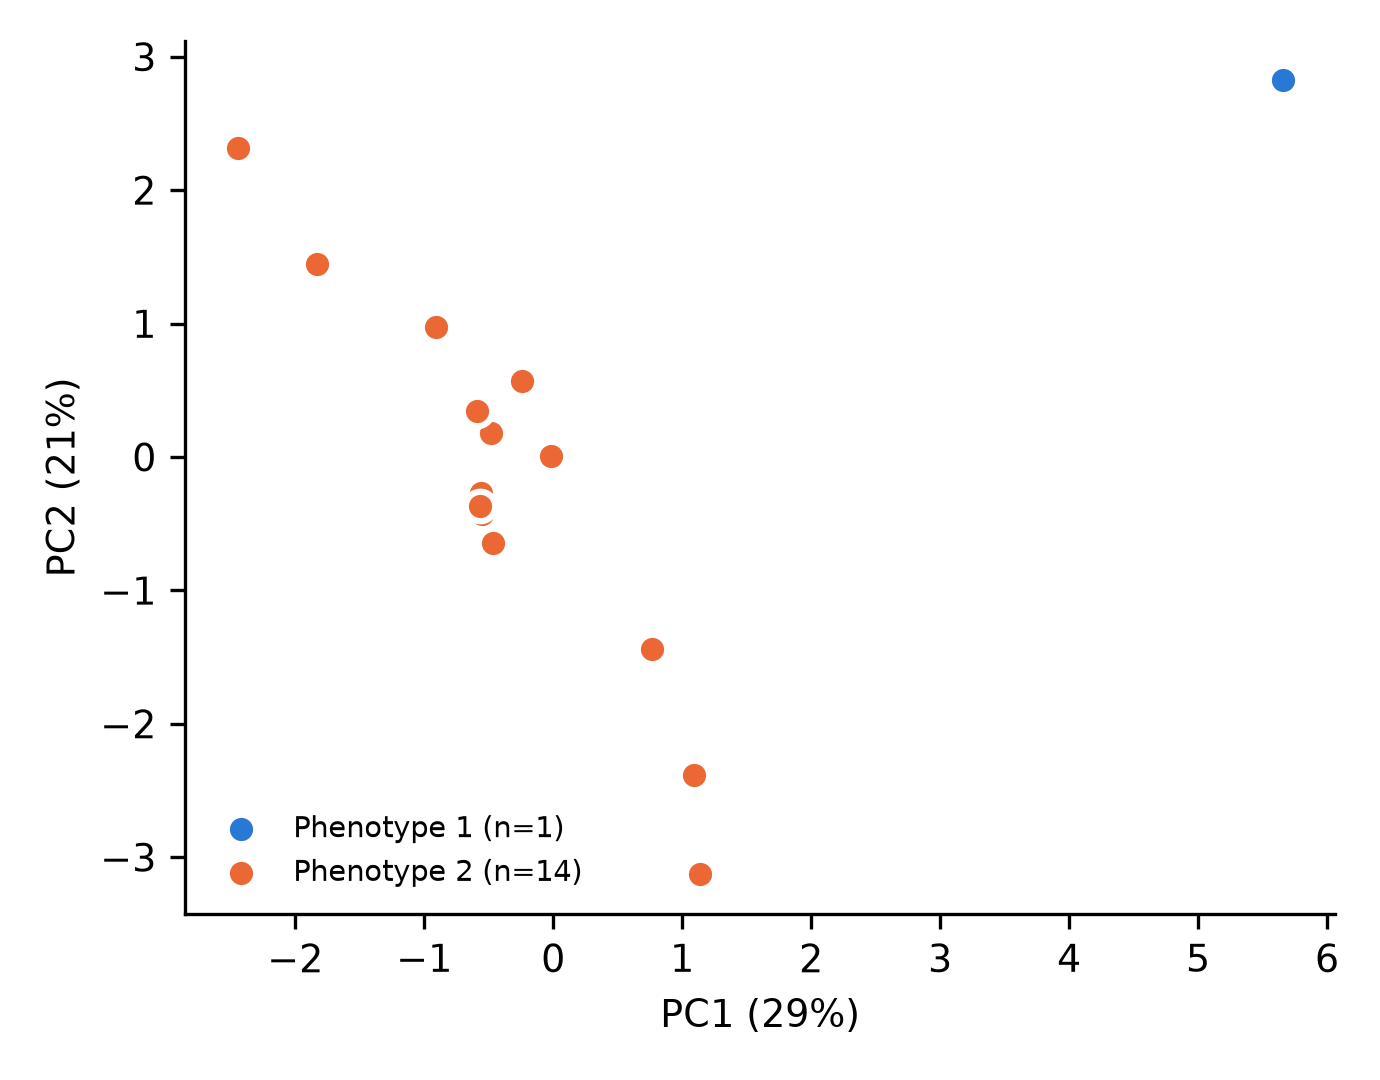
\includegraphics[width=0.6\linewidth,height=\textheight,keepaspectratio,alt={Case-report phenotypes: NAION case patients from case reports and series projected onto the first two principal components (PC1, PC2; percentage of variance explained in parentheses) of standardized clinical features. Colours = k-means clusters at the best silhouette solution (k = 2); one cluster contains a single tirzepatide-treated patient, so no stable multi-patient phenotype was found. Remaining abbreviations and variable names: Nomenclature appendix.}]{figures/fig_case_phenotypes_pca.png}
\caption{Case-report phenotypes: NAION case patients from case reports
and series projected onto the first two principal components (PC1, PC2;
percentage of variance explained in parentheses) of standardized
clinical features. Colours = k-means clusters at the best silhouette
solution (k = 2); one cluster contains a single tirzepatide-treated
patient, so no stable multi-patient phenotype was found. Remaining
abbreviations and variable names: Nomenclature appendix.}
\end{figure}

\begin{figure}
\centering
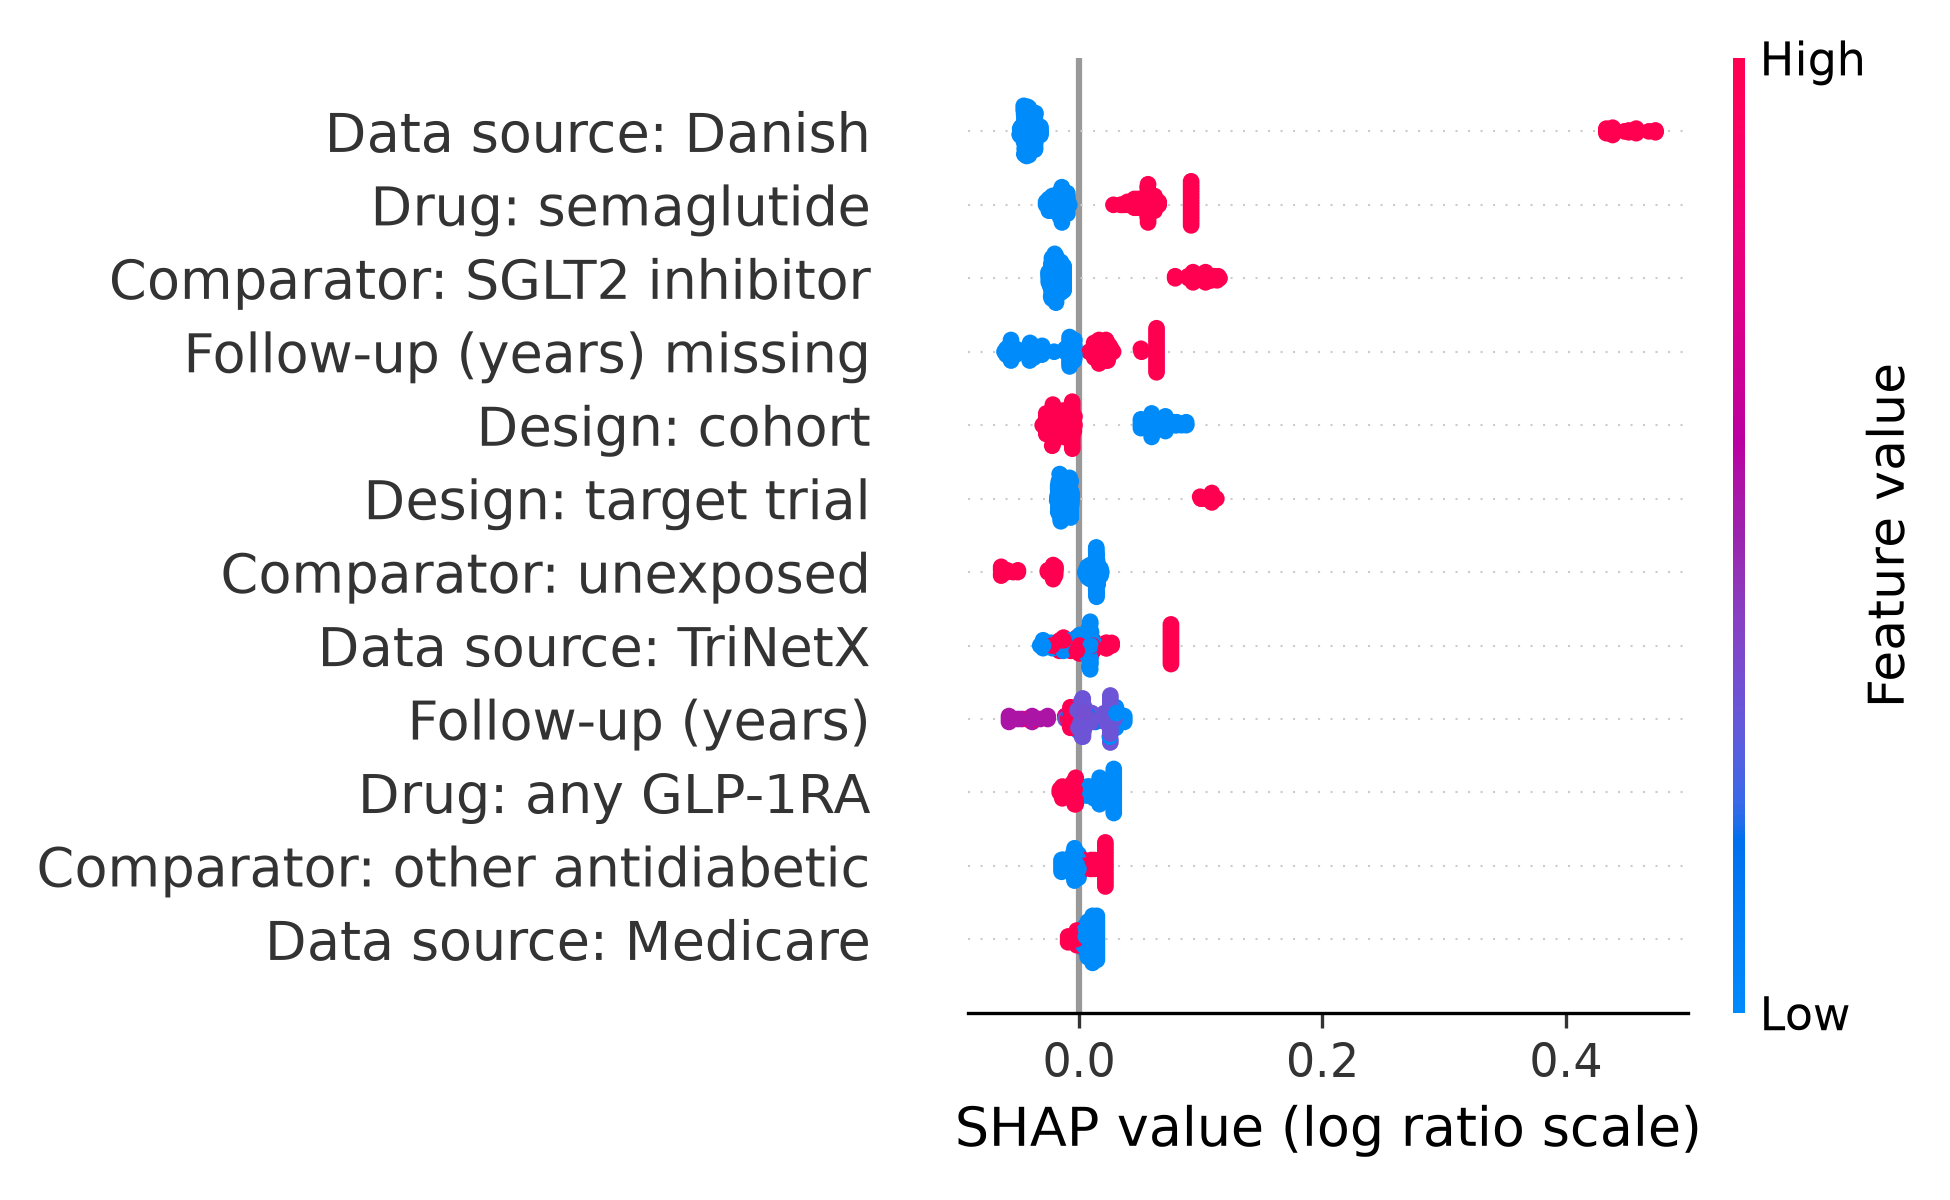
\includegraphics[width=0.8\linewidth,height=\textheight,keepaspectratio,alt={SHAP summary for the random-forest meta-regression of 148 published log ratio estimates from 25 studies. Each dot is one published estimate; the x-axis is its SHAP value on the log-ratio scale; colour is the feature value (red = 1 or high, blue = 0 or low). Features describe the publication: dataset\_ (data source, e.g., danish = Danish registries, trinetx = TriNetX network, medicare = Medicare claims), design\_ (cohort or target-trial emulation), comparator\_cls\_ (comparator class), exposure\_drug\_ (exposure drug), followup (years) and followup\_missing (not reported). Remaining abbreviations and variable names: Nomenclature appendix.}]{figures/fig_meta_shap.png}
\caption{SHAP summary for the random-forest meta-regression of 148
published log ratio estimates from 25 studies. Each dot is one published
estimate; the x-axis is its SHAP value on the log-ratio scale; colour is
the feature value (red = 1 or high, blue = 0 or low). Features describe
the publication: dataset\_ (data source, e.g., danish = Danish
registries, trinetx = TriNetX network, medicare = Medicare claims),
design\_ (cohort or target-trial emulation), comparator\_cls\_
(comparator class), exposure\_drug\_ (exposure drug), followup (years)
and followup\_missing (not reported). Remaining abbreviations and
variable names: Nomenclature appendix.}
\end{figure}

\section{Graph neural networks}\label{graph-neural-networks-1}

The GraphSAGE GNN reached an AUROC of 0.649 \ensuremath{\pm} 0.014 across the 10 folds,
not different from XGBoost on identical splits (difference -0.0077;
P=0.779), with O/E 1.01. In leave-one-study-out validation its AUROC was
0.531 (P=0.034 vs 0.5). Integrated-gradient attributions ranked therapy,
data source and region highest, mirroring SHAP.

Nested tuning over 366 GNN configurations selected a SAGE network of
depth 6 with k=20 neighbours, uniform edge weighting and same-study
weight 5.0; on the untouched folds it differed from the default network
by 0.0006 AUROC (P=0.948).

\begin{figure}
\centering
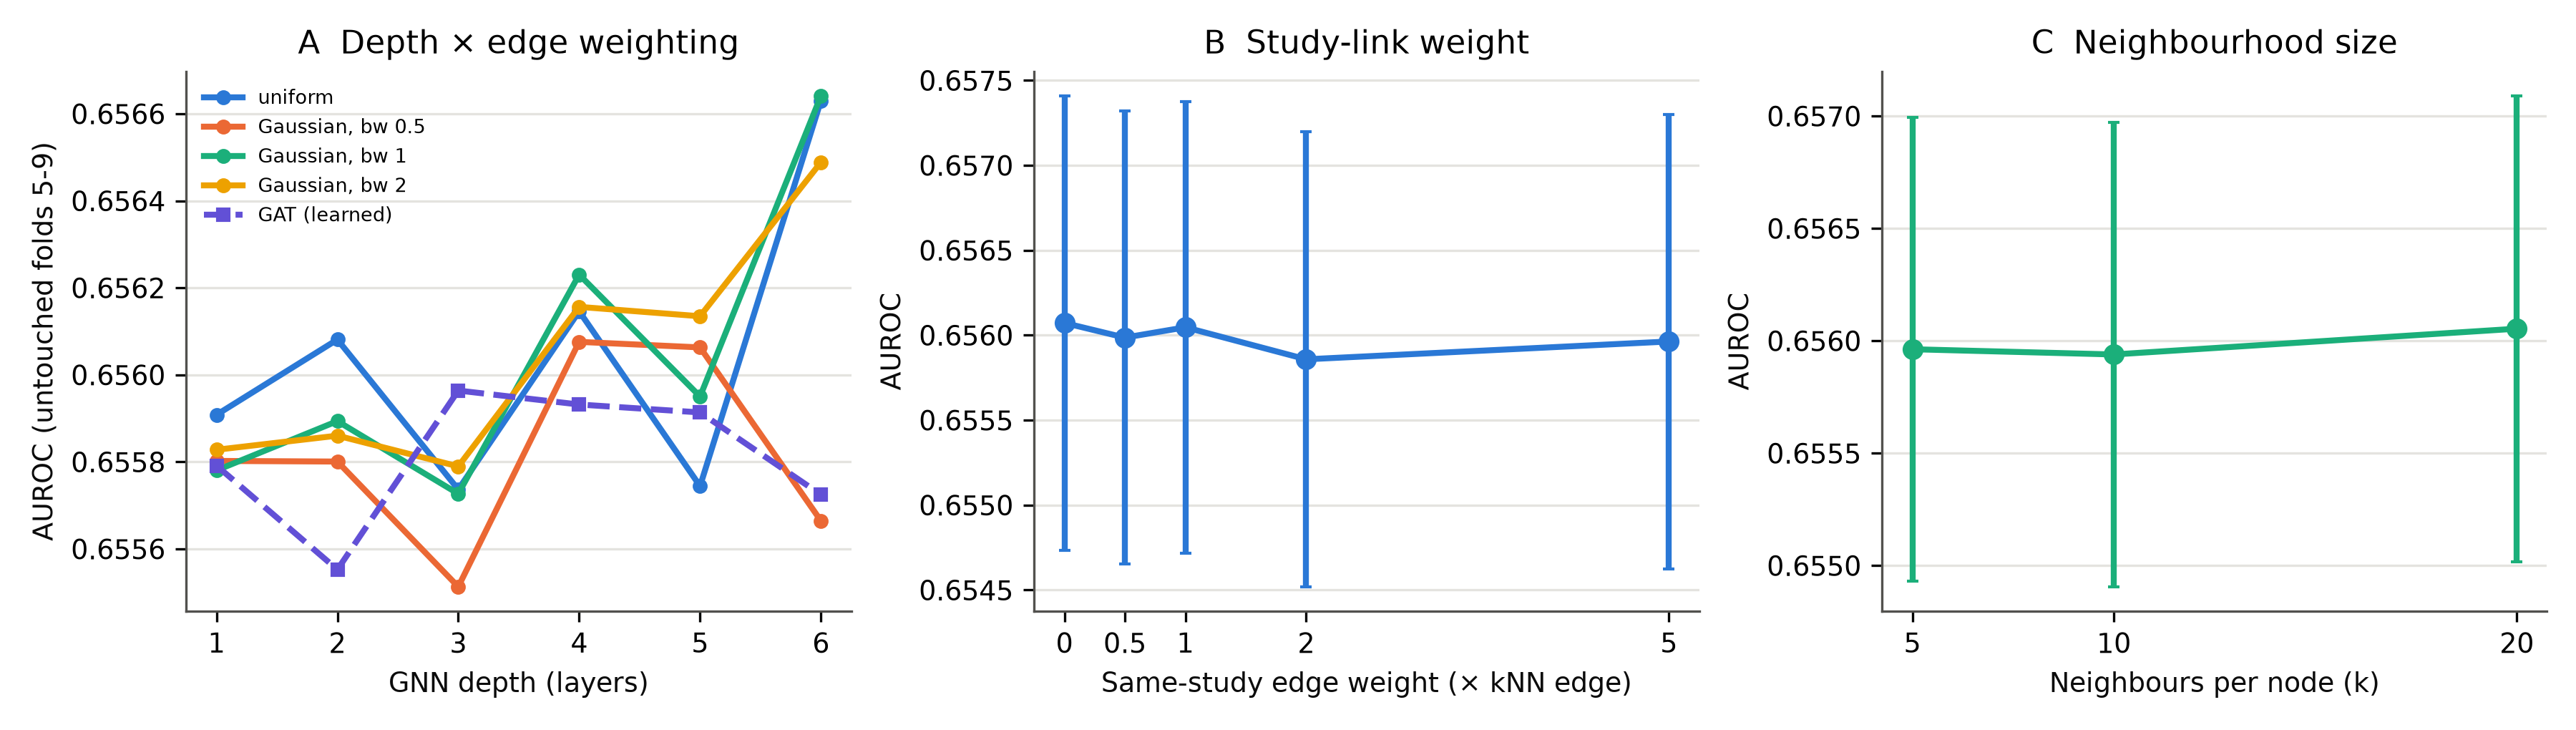
\includegraphics[width=1\linewidth,height=\textheight,keepaspectratio,alt={Graph neural network tuning, evaluated on untouched folds 5 to 9 (AUROC). (A) Network depth (1 to 6 message-passing layers) by edge weighting: uniform = all k-nearest-neighbour edges weight 1; gauss0.5, gauss1, gauss2 = Gaussian kernel of feature distance with bandwidth 0.5, 1 or 2; dashed = graph attention network (GAT) with learned weights. (B) Weight of same-study edges as a multiple of a k-nearest-neighbour edge. (C) Number of neighbours per node (k). Points = mean; bars = SD across folds. All differences are smaller than 0.002 AUROC. Remaining abbreviations and variable names: Nomenclature appendix.}]{figures/fig_gnn_depth_weights.png}
\caption{Graph neural network tuning, evaluated on untouched folds 5 to
9 (AUROC). (A) Network depth (1 to 6 message-passing layers) by edge
weighting: uniform = all k-nearest-neighbour edges weight 1; gauss0.5,
gauss1, gauss2 = Gaussian kernel of feature distance with bandwidth 0.5,
1 or 2; dashed = graph attention network (GAT) with learned weights. (B)
Weight of same-study edges as a multiple of a k-nearest-neighbour edge.
(C) Number of neighbours per node (k). Points = mean; bars = SD across
folds. All differences are smaller than 0.002 AUROC. Remaining
abbreviations and variable names: Nomenclature appendix.}
\end{figure}

\section{Ensembles (including the
GNN)}\label{ensembles-including-the-gnn}

Among 11 member combinations \ensuremath{\times} 3 combiners, the best ensemble
(cross\_family(pubmed+hybrid+synthetic), mean) reached AUROC 0.657, a
difference of 0.0010 from the best single model (q=1.000).

\section{Synthetic digital twins (factorial grid with local
refinement)}\label{synthetic-digital-twins-factorial-grid-with-local-refinement}

In the XGBoost grid (5,310 fits), no hybrid cell improved AUROC over
PubMed-only training (0 of 162 cells with a confidence interval above
zero); the best hybrid changed AUROC by 0.0009 (95\% CI, -0.0004 to
0.0022), synthetic-only training with twins fitted to real data lost
0.010, and twins built only from published priors reached AUROC values
near 0.55. Adding twins beyond about 9 to 27 times the real training
size reduced performance.

\begin{figure}
\centering
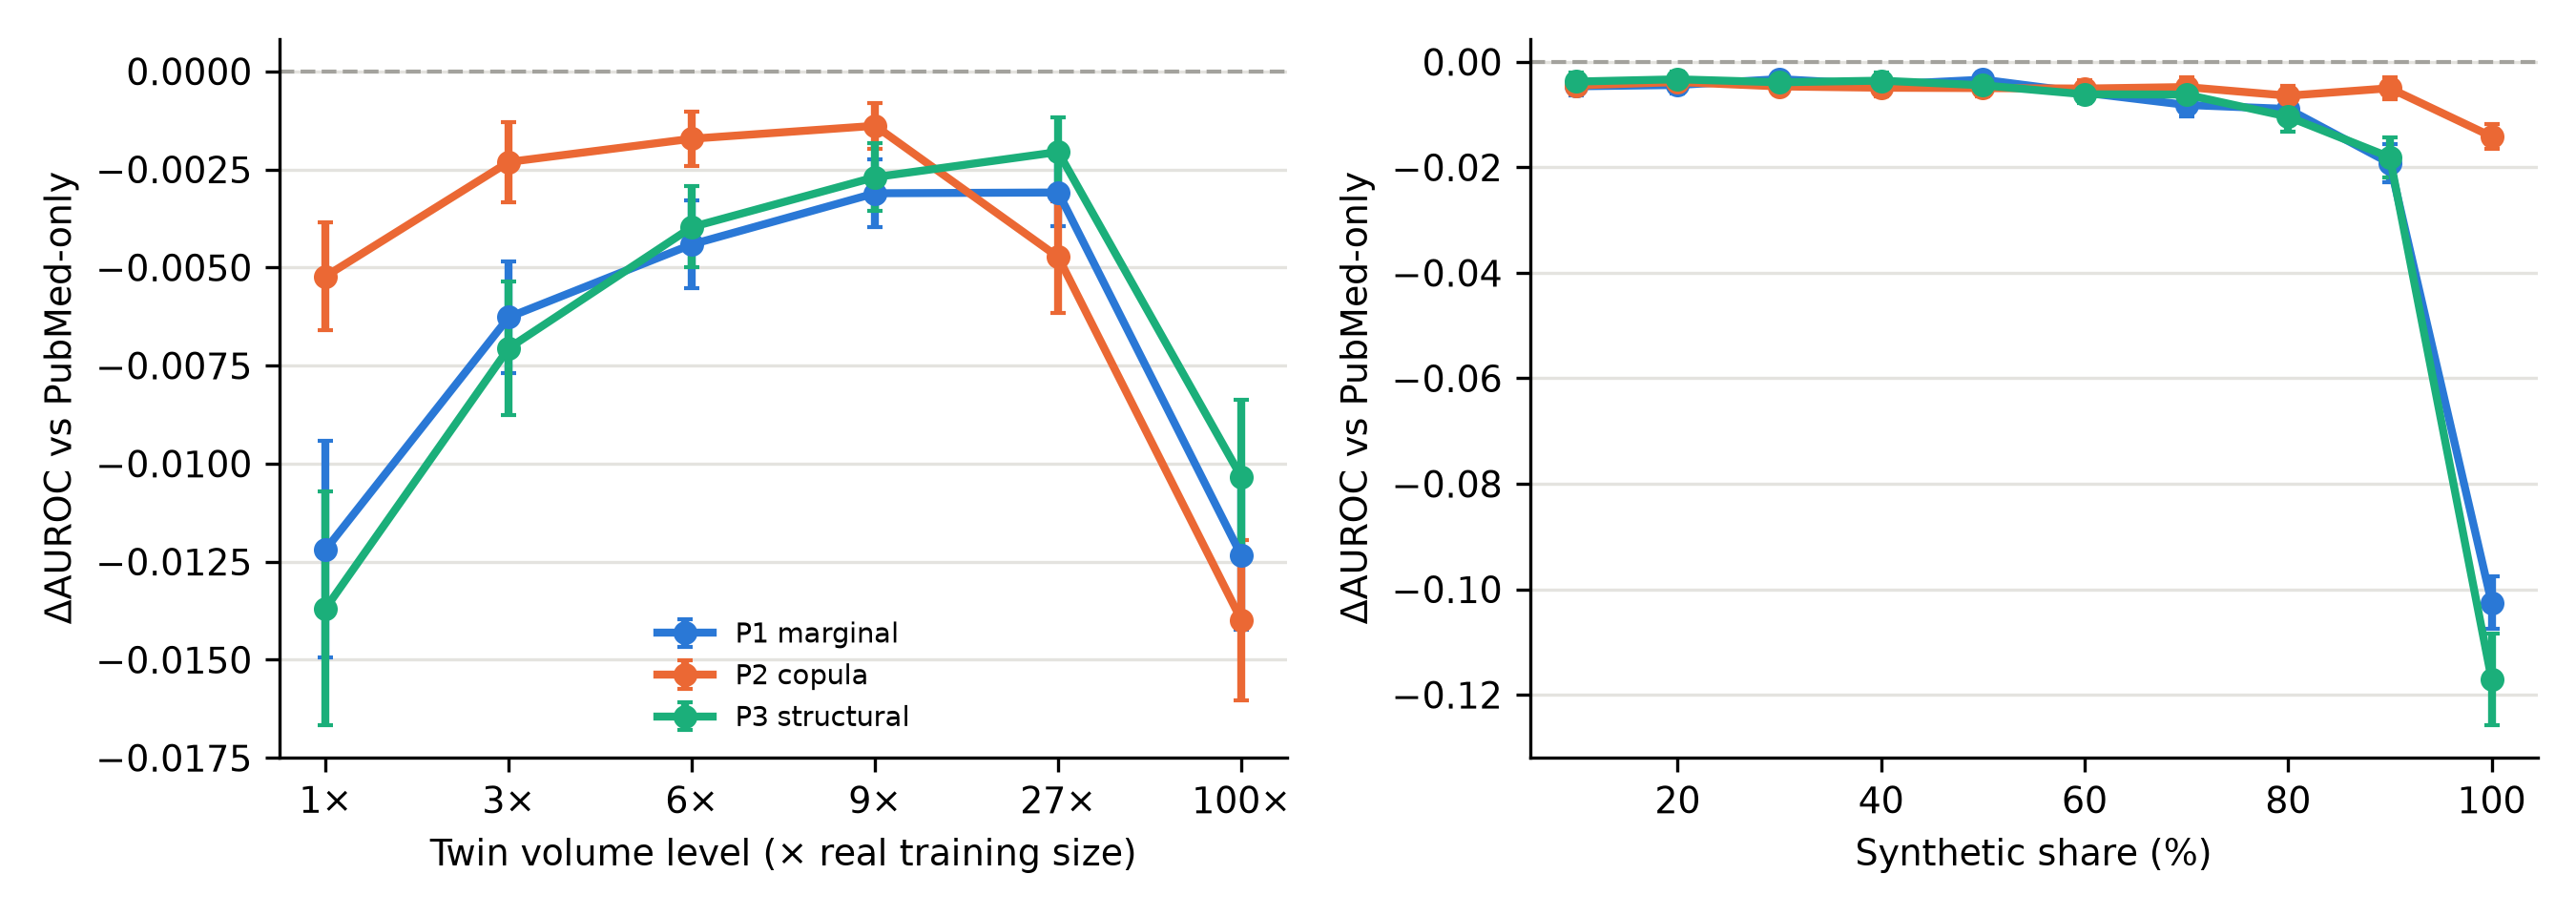
\includegraphics[width=1\linewidth,height=\textheight,keepaspectratio,alt={Synthetic-data grid (Stage 2, XGBoost): change in AUROC versus PubMed-only training on the same split (mean and 95\% CI over grid cells and seeds). Left, by synthetic volume (multiples of the real training size); right, by synthetic share of the training set. Blue, marginal generator; orange, Gaussian-copula generator; green, structural (logistic) generator. Dashed line = no change; values below zero mean synthetic data reduced discrimination. Remaining abbreviations and variable names: Nomenclature appendix.}]{figures/fig_volume_share_response.png}
\caption{Synthetic-data grid (Stage 2, XGBoost): change in AUROC versus
PubMed-only training on the same split (mean and 95\% CI over grid cells
and seeds). Left, by synthetic volume (multiples of the real training
size); right, by synthetic share of the training set. Blue, marginal
generator; orange, Gaussian-copula generator; green, structural
(logistic) generator. Dashed line = no change; values below zero mean
synthetic data reduced discrimination. Remaining abbreviations and
variable names: Nomenclature appendix.}
\end{figure}

\begin{figure}
\centering
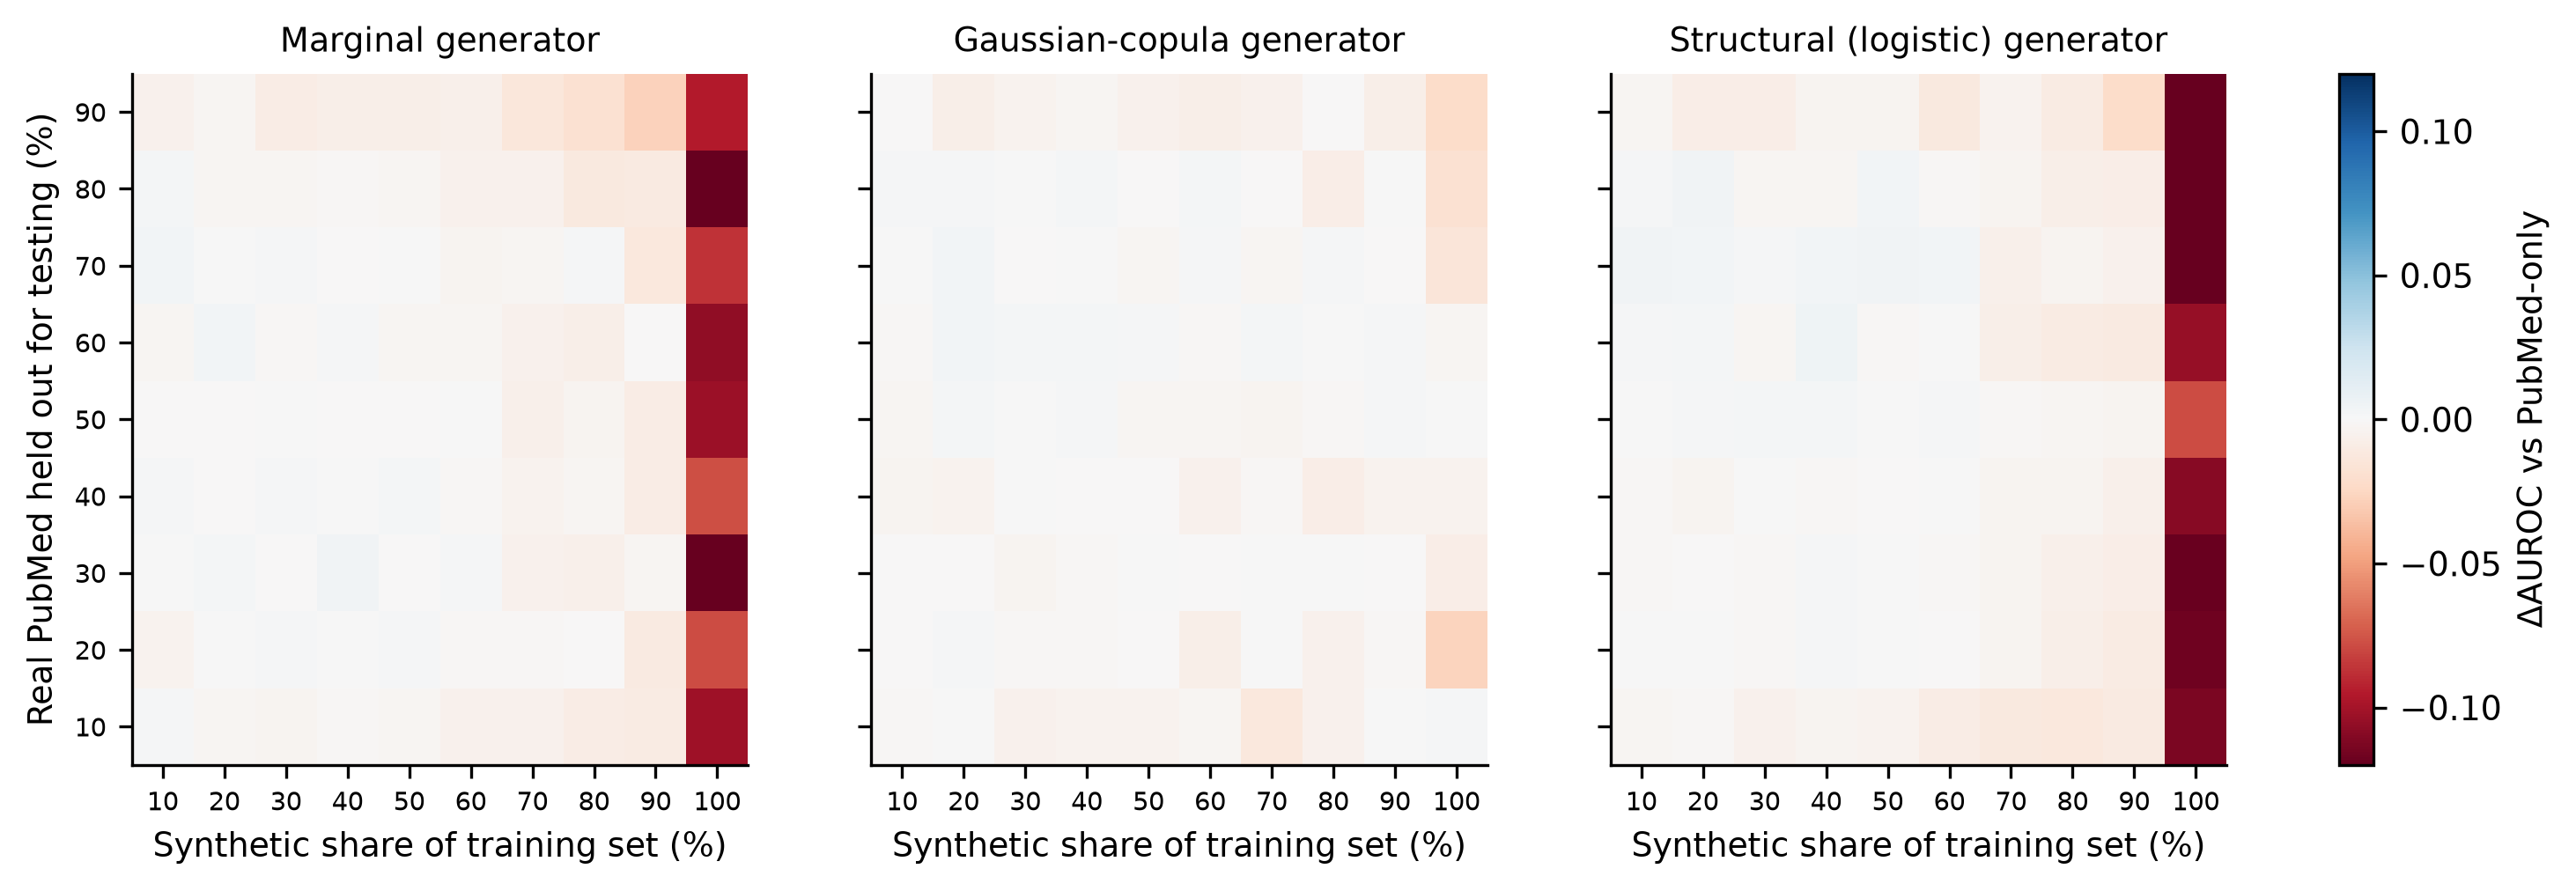
\includegraphics[width=1\linewidth,height=\textheight,keepaspectratio,alt={Synthetic-data grid at 9x volume: change in AUROC versus PubMed-only training (colour; red = worse, blue = better) by synthetic share of the training set (columns) and percentage of real PubMed data held out for testing (rows), for each generator. Training sets made entirely of synthetic data (100\% share) lose the most. Remaining abbreviations and variable names: Nomenclature appendix.}]{figures/fig_heatmap_share_heldout_V9.png}
\caption{Synthetic-data grid at 9x volume: change in AUROC versus
PubMed-only training (colour; red = worse, blue = better) by synthetic
share of the training set (columns) and percentage of real PubMed data
held out for testing (rows), for each generator. Training sets made
entirely of synthetic data (100\% share) lose the most. Remaining
abbreviations and variable names: Nomenclature appendix.}
\end{figure}

Across the full factorial grid (45,360 configurations), 4452 hybrid or
synthetic configurations improved discrimination over PubMed-only
training after Benjamini-Hochberg correction.

\begin{figure}
\centering
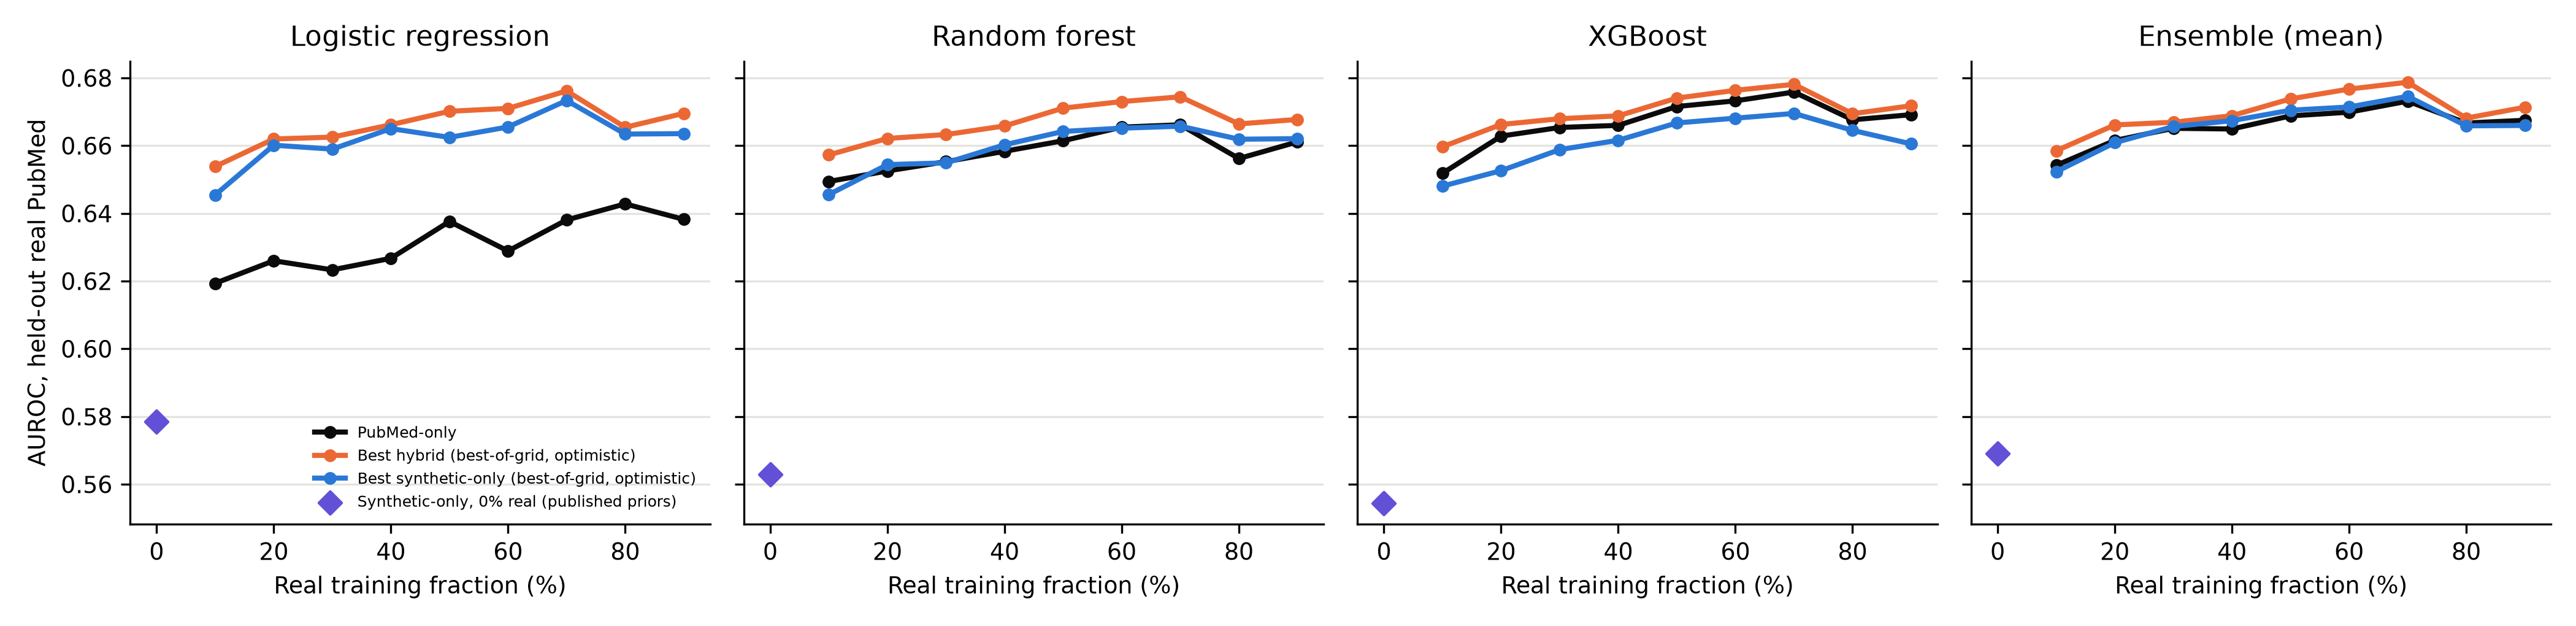
\includegraphics[width=1\linewidth,height=\textheight,keepaspectratio,alt={Full factorial experiment: AUROC on held-out real PubMed data versus the real training fraction, for each model. Black, PubMed-only training; orange, best hybrid (real plus synthetic) configuration; blue, best synthetic-only configuration; both selected as the best of the grid and therefore optimistic. Purple diamond at 0\% real data: synthetic-only training from published priors alone. Remaining abbreviations and variable names: Nomenclature appendix.}]{figures/fig_learning_curves_families.png}
\caption{Full factorial experiment: AUROC on held-out real PubMed data
versus the real training fraction, for each model. Black, PubMed-only
training; orange, best hybrid (real plus synthetic) configuration; blue,
best synthetic-only configuration; both selected as the best of the grid
and therefore optimistic. Purple diamond at 0\% real data:
synthetic-only training from published priors alone. Remaining
abbreviations and variable names: Nomenclature appendix.}
\end{figure}

\begin{figure}
\centering
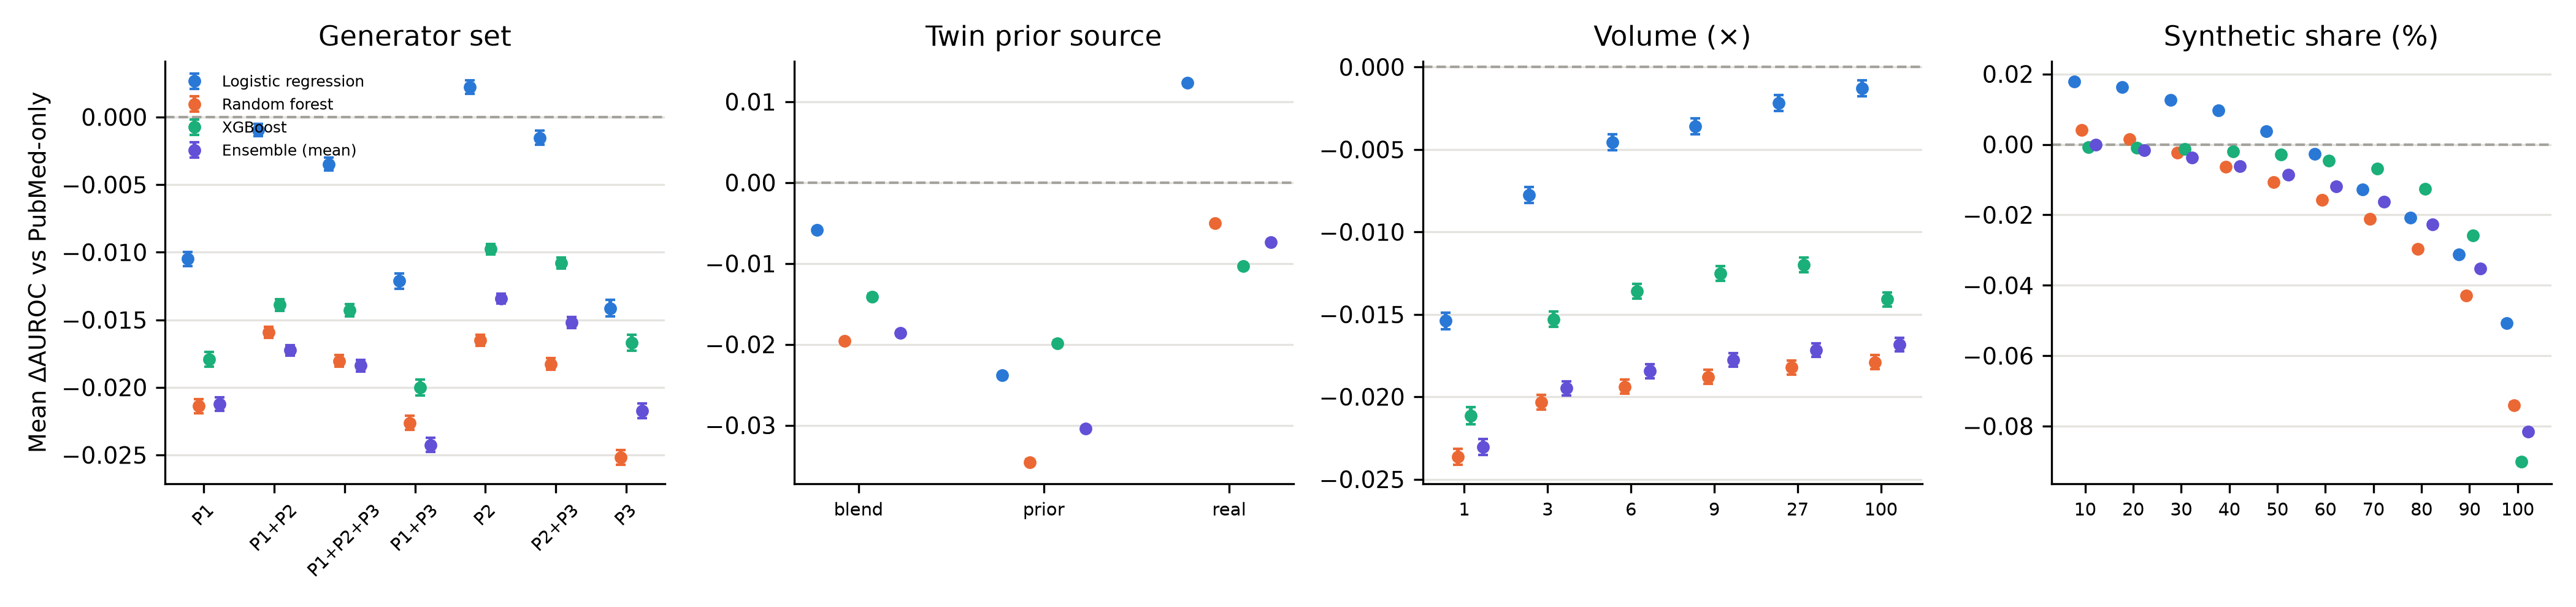
\includegraphics[width=1\linewidth,height=\textheight,keepaspectratio,alt={Full factorial experiment: main effect of each design factor on AUROC relative to PubMed-only training (mean change and 95\% CI, averaged over all other factors), by model (blue, logistic regression; orange, random forest; green, XGBoost; purple, mean ensemble). Generator set: Marg = marginal, Cop = Gaussian copula, Struct = structural (logistic), joined by + when combined. Prior source: real = fitted to the real training split; prior = published estimates only; blend = 50/50. Volume = synthetic records as a multiple of the real training size. Synthetic share = percentage of the training set that is synthetic. Dashed line = no change. Remaining abbreviations and variable names: Nomenclature appendix.}]{figures/fig_main_effects.png}
\caption{Full factorial experiment: main effect of each design factor on
AUROC relative to PubMed-only training (mean change and 95\% CI,
averaged over all other factors), by model (blue, logistic regression;
orange, random forest; green, XGBoost; purple, mean ensemble). Generator
set: Marg = marginal, Cop = Gaussian copula, Struct = structural
(logistic), joined by + when combined. Prior source: real = fitted to
the real training split; prior = published estimates only; blend =
50/50. Volume = synthetic records as a multiple of the real training
size. Synthetic share = percentage of the training set that is
synthetic. Dashed line = no change. Remaining abbreviations and variable
names: Nomenclature appendix.}
\end{figure}

\section{Model summary}\label{model-summary}

{\footnotesize
\begin{longtable}[]{@{}
  >{\raggedright\arraybackslash}p{(\linewidth - 14\tabcolsep) * \real{0.3500}}
  >{\raggedright\arraybackslash}p{(\linewidth - 14\tabcolsep) * \real{0.1150}}
  >{\raggedright\arraybackslash}p{(\linewidth - 14\tabcolsep) * \real{0.0750}}
  >{\raggedright\arraybackslash}p{(\linewidth - 14\tabcolsep) * \real{0.1550}}
  >{\raggedright\arraybackslash}p{(\linewidth - 14\tabcolsep) * \real{0.0700}}
  >{\raggedright\arraybackslash}p{(\linewidth - 14\tabcolsep) * \real{0.0350}}
  >{\raggedright\arraybackslash}p{(\linewidth - 14\tabcolsep) * \real{0.1050}}
  >{\raggedright\arraybackslash}p{(\linewidth - 14\tabcolsep) * \real{0.0950}}@{}}
\caption{Model performance by family. AUROC 10/90 = trained on 10\%,
tested on 90\%; AUROC 10x10\% folds = mean \ensuremath{\pm} SD over ten disjoint folds;
AUROC LOSO = leave-one-study-out; O/E = observed/expected events;
Sens/Spec and PPV/NPV at the top-10\% threshold; hybrid = real plus
synthetic training data; synthetic only = no real training data; priors
= published estimates used to generate synthetic data. Remaining
abbreviations and variable names: Nomenclature
appendix.\label{tbl:models}}\tabularnewline
\toprule\noalign{}
\begin{minipage}[b]{\linewidth}\raggedright
Model
\end{minipage} & \begin{minipage}[b]{\linewidth}\raggedright
Training data
\end{minipage} & \begin{minipage}[b]{\linewidth}\raggedright
AUROC 10/90
\end{minipage} & \begin{minipage}[b]{\linewidth}\raggedright
AUROC 10\ensuremath{\times}10\% folds
\end{minipage} & \begin{minipage}[b]{\linewidth}\raggedright
AUROC LOSO
\end{minipage} & \begin{minipage}[b]{\linewidth}\raggedright
O/E
\end{minipage} & \begin{minipage}[b]{\linewidth}\raggedright
Sens/Spec top 10\%
\end{minipage} & \begin{minipage}[b]{\linewidth}\raggedright
PPV/NPV top 10\%
\end{minipage} \\
\midrule\noalign{}
\endfirsthead
\toprule\noalign{}
\begin{minipage}[b]{\linewidth}\raggedright
Model
\end{minipage} & \begin{minipage}[b]{\linewidth}\raggedright
Training data
\end{minipage} & \begin{minipage}[b]{\linewidth}\raggedright
AUROC 10/90
\end{minipage} & \begin{minipage}[b]{\linewidth}\raggedright
AUROC 10\ensuremath{\times}10\% folds
\end{minipage} & \begin{minipage}[b]{\linewidth}\raggedright
AUROC LOSO
\end{minipage} & \begin{minipage}[b]{\linewidth}\raggedright
O/E
\end{minipage} & \begin{minipage}[b]{\linewidth}\raggedright
Sens/Spec top 10\%
\end{minipage} & \begin{minipage}[b]{\linewidth}\raggedright
PPV/NPV top 10\%
\end{minipage} \\
\midrule\noalign{}
\endhead
\bottomrule\noalign{}
\endlastfoot
Logistic regression (L2) & PubMed only & 0.627 & 0.616 \ensuremath{\pm} 0.010 & 0.528 &
1.01 & 0.26/0.85 & 0.075\%/99.96\% \\
Random forest & PubMed only & 0.642 & 0.646 \ensuremath{\pm} 0.014 & 0.531 & 1.00 &
0.31/0.85 & 0.096\%/99.96\% \\
XGBoost & PubMed only & 0.657 & 0.656 \ensuremath{\pm} 0.011 & 0.534 & 1.00 & 0.35/0.82
& 0.087\%/99.97\% \\
Mean ensemble (LR+RF+XGB) & PubMed only & 0.657 & 0.656 \ensuremath{\pm} 0.011 & --- &
--- & 0.31/0.86 & 0.101\%/99.97\% \\
GNN (GraphSAGE, 2 layers) & PubMed only & 0.647 & 0.649 \ensuremath{\pm} 0.014 & 0.531
& 1.01 & 0.35/0.82 & 0.086\%/99.97\% \\
GNN tuned (SAGE, depth 6, k=20, uniform, study weight 5.0) & PubMed only
& --- & 0.657 (untouched folds) & 0.541 & 1.03 & --- & --- \\
XGBoost (PubMed only) & PubMed only & --- & 0.667 (all fractions) & ---
& 1.00 & --- & --- \\
XGBoost --- hybrid (copula + structural generators, published priors,
100\ensuremath{\times}, 10\% synthetic) & Hybrid & --- & 0.669 (all fractions) & --- &
1.01 & --- & --- \\
Mean ensemble --- synthetic only (copula generator, real-data priors,
9\ensuremath{\times}, 100\% synthetic) & Synthetic only & --- & 0.664 (all fractions) &
--- & 1.01 & --- & --- \\
Mean ensemble --- synthetic only, 0\% real (copula generator, 100\ensuremath{\times}) &
Published priors only & --- & 0.569 (all real data as test) & --- & 1.11
& --- & --- \\
Ensemble cross-family (PubMed-only + hybrid + synthetic-only) (mean) &
PubMed only & --- & 0.657 \ensuremath{\pm} 0.010 & --- & 1.01 & --- & --- \\
Ensemble LR+XGBoost (mean) & PubMed only & --- & 0.657 \ensuremath{\pm} 0.008 & --- &
1.00 & --- & --- \\
\end{longtable}
}

\section{Data modalities and multimodal
feasibility}\label{data-modalities-and-multimodal-feasibility}

\begin{table}[!htbp]\centering\caption{Data modalities available for modelling and their use. CNN,
convolutional neural network; Grad-CAM, gradient-weighted class
activation mapping; OCT, optical coherence tomography. Remaining
abbreviations and variable names: Nomenclature appendix.}\scriptsize
\maxwbox{\textwidth}{\begin{tabular}{llll}\toprule
Modality & Available & Amount & Use / feasibility \\
\midrule
Structured tabular (categorical + numeric) & Yes & 3.27 million reconstructed patients & All supervised, graph, CNN-1D and twin models \\
Free text (abstracts, full texts) & Yes & 169 records; 60 full texts & Extraction only; too few labelled patients for text models \\
Images (fundus, OCT, visual fields, MRI) & Figures only & about 6 patients with pre/post figures & Not trainable; 2D/3D CNN + Grad-CAM pipeline prepared \\
3D volumes (OCT cubes) & No & 0 & Not available \\
Video / time series & No & 0 & Not available \\
\bottomrule\end{tabular}}
\end{table}

\begin{figure}
\centering
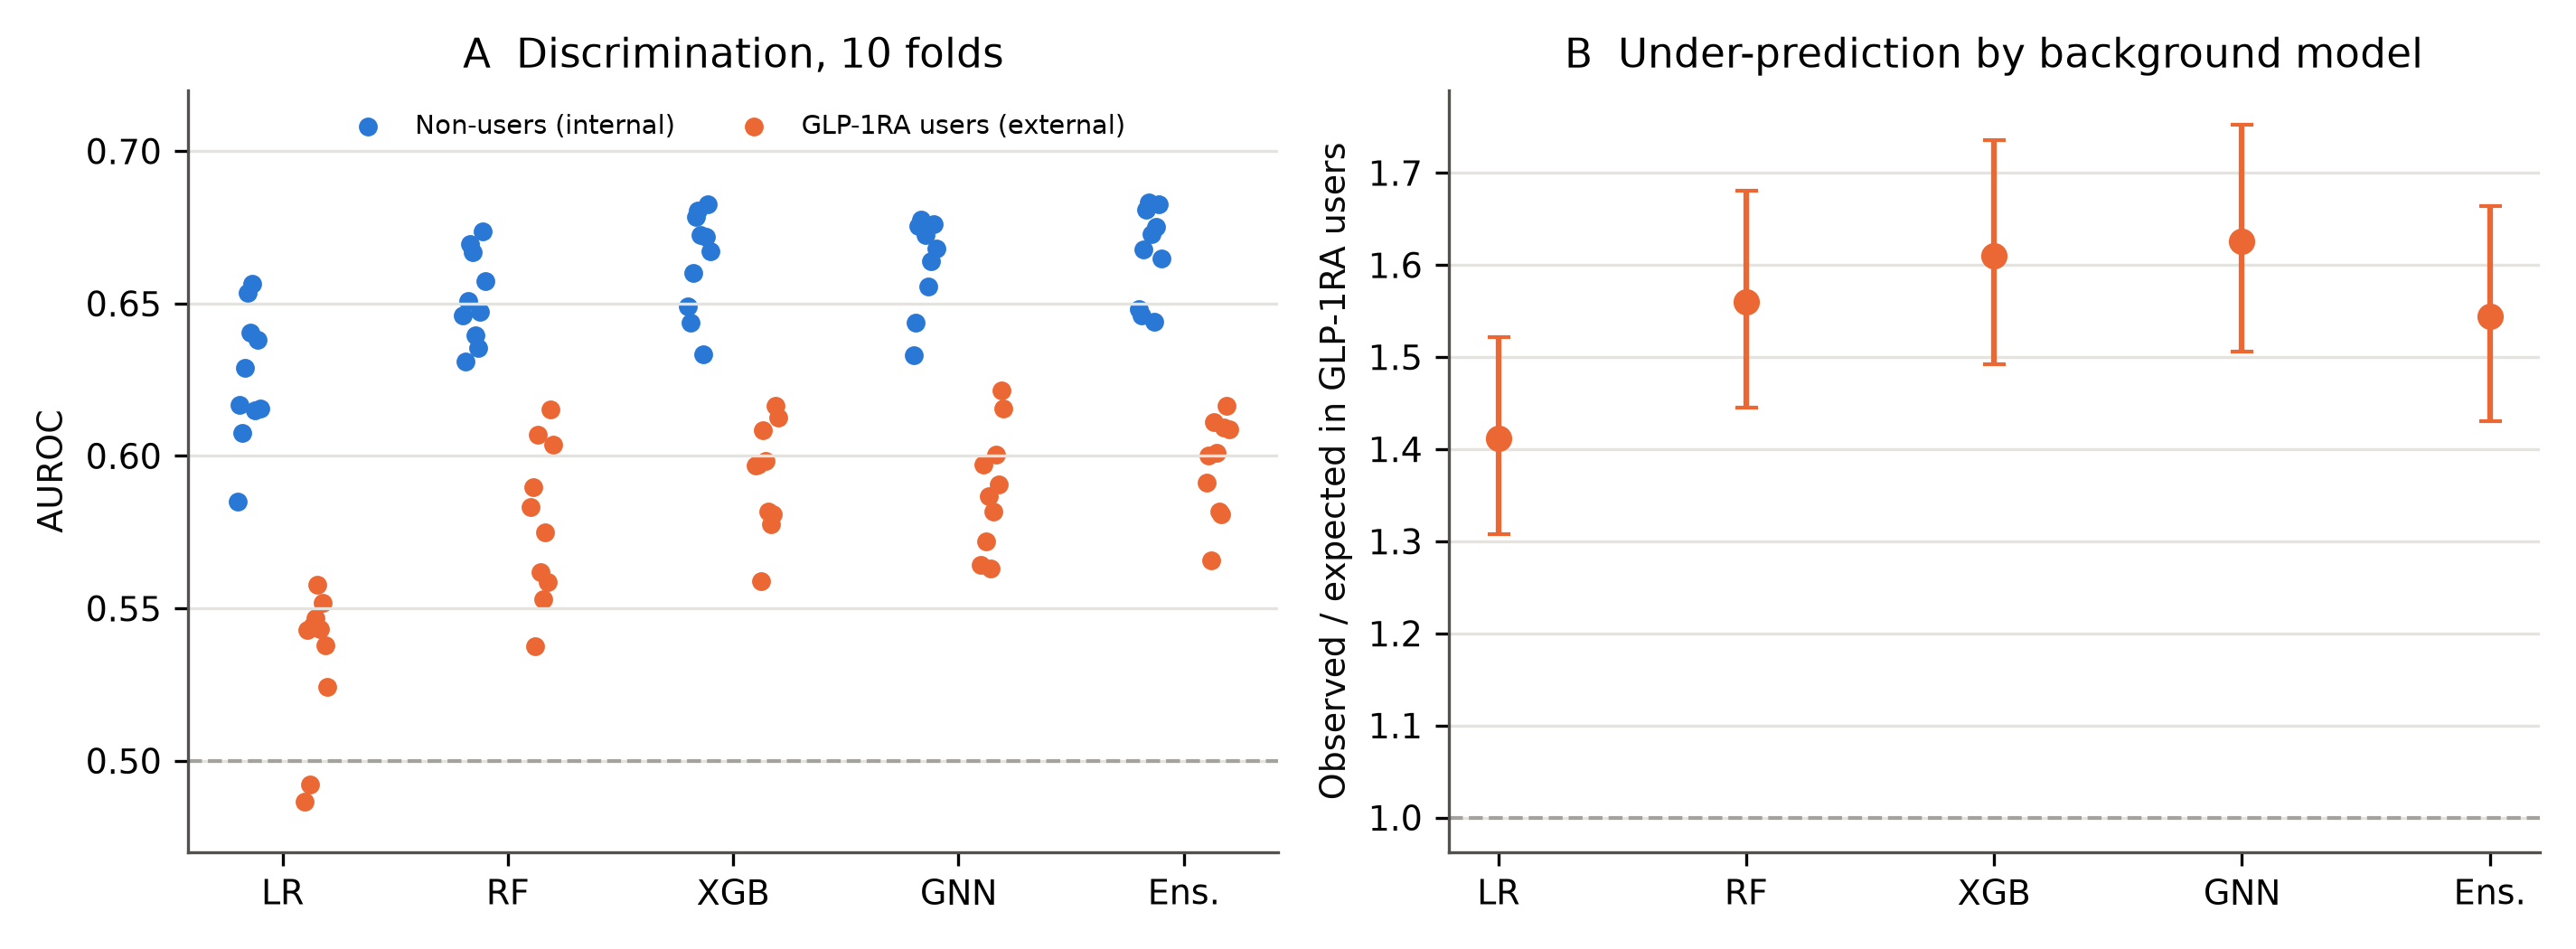
\includegraphics[width=1\linewidth,height=\textheight,keepaspectratio,alt={Background-risk models trained only on non-users and applied to GLP-1 receptor agonist users. (A) AUROC per fold: blue, internal validation in held-out non-users; orange, external validation in GLP-1RA users; dashed line = chance. (B) Observed/expected (O/E) NAION events in GLP-1RA users (mean and 95\% CI); values above the dashed line at 1 mean the non-user model under-predicts risk in users. LR, logistic regression; RF, random forest; XGB, XGBoost; GNN, graph neural network; Ens., mean ensemble. Remaining abbreviations and variable names: Nomenclature appendix.}]{figures/fig_stage7_external.png}
\caption{Background-risk models trained only on non-users and applied to
GLP-1 receptor agonist users. (A) AUROC per fold: blue, internal
validation in held-out non-users; orange, external validation in GLP-1RA
users; dashed line = chance. (B) Observed/expected (O/E) NAION events in
GLP-1RA users (mean and 95\% CI); values above the dashed line at 1 mean
the non-user model under-predicts risk in users. LR, logistic
regression; RF, random forest; XGB, XGBoost; GNN, graph neural network;
Ens., mean ensemble. Remaining abbreviations and variable names:
Nomenclature appendix.}
\end{figure}

\begin{figure}
\centering
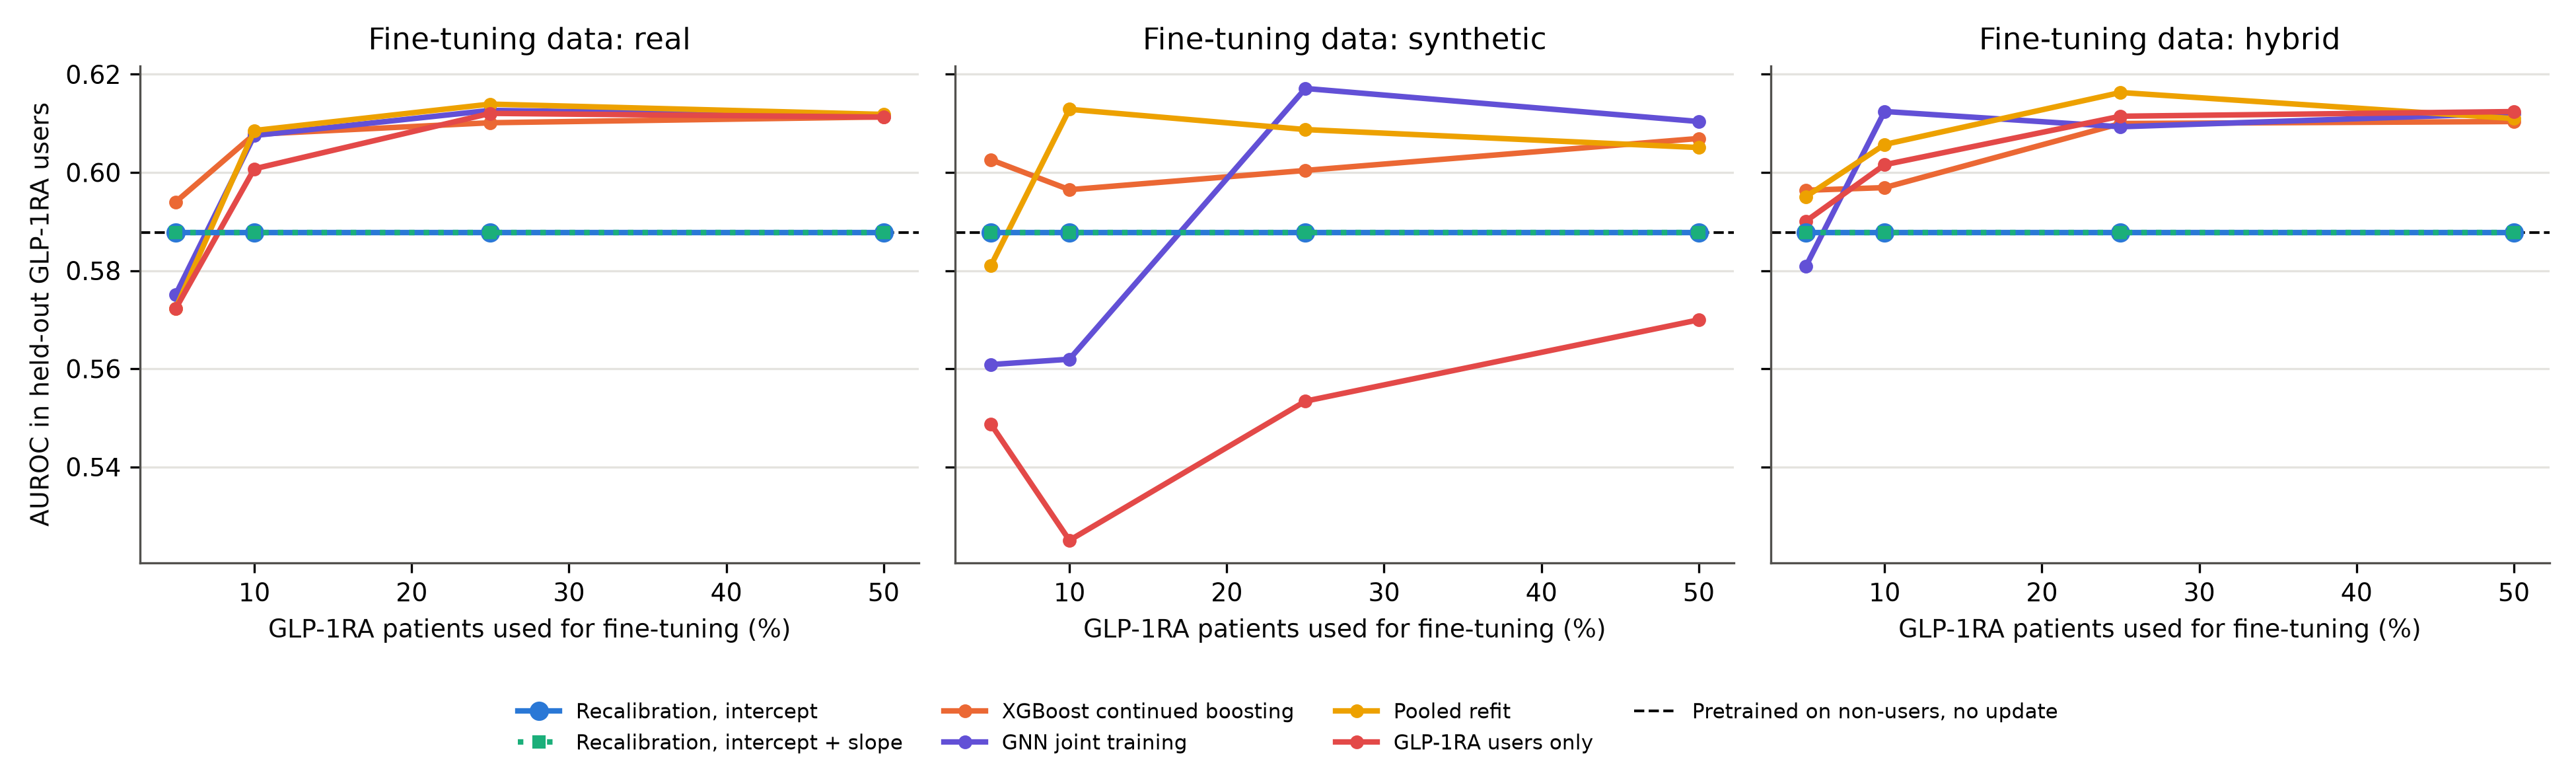
\includegraphics[width=1\linewidth,height=\textheight,keepaspectratio,alt={Fine-tuning a non-user model for GLP-1RA users: AUROC in held-out GLP-1RA users versus the percentage of GLP-1RA users used for fine-tuning, by fine-tuning data source (real, synthetic or hybrid). Lines = update methods (legend below the panels). Recalibration (intercept only, or intercept and slope) is a monotone transformation of the risk score, so it cannot change AUROC; both recalibration lines therefore lie on the dashed line (pretrained non-user model without update). GLP-1RA users only = model trained on GLP-1RA users without pretraining. Remaining abbreviations and variable names: Nomenclature appendix.}]{figures/fig_finetune.png}
\caption{Fine-tuning a non-user model for GLP-1RA users: AUROC in
held-out GLP-1RA users versus the percentage of GLP-1RA users used for
fine-tuning, by fine-tuning data source (real, synthetic or hybrid).
Lines = update methods (legend below the panels). Recalibration
(intercept only, or intercept and slope) is a monotone transformation of
the risk score, so it cannot change AUROC; both recalibration lines
therefore lie on the dashed line (pretrained non-user model without
update). GLP-1RA users only = model trained on GLP-1RA users without
pretraining. Remaining abbreviations and variable names: Nomenclature
appendix.}
\end{figure}

\section{Reporting checklist}\label{reporting-checklist}

{\footnotesize
\begin{longtable}[]{@{}
  >{\raggedright\arraybackslash}p{(\linewidth - 2\tabcolsep) * \real{0.1714}}
  >{\raggedright\arraybackslash}p{(\linewidth - 2\tabcolsep) * \real{0.8286}}@{}}
\caption{TRIPOD+AI reporting items (Transparent Reporting of a
multivariable prediction model for Individual Prognosis Or Diagnosis, AI
extension) and where each is addressed. Remaining abbreviations and
variable names: Nomenclature appendix.}\tabularnewline
\toprule\noalign{}
\begin{minipage}[b]{\linewidth}\raggedright
TRIPOD+AI domain
\end{minipage} & \begin{minipage}[b]{\linewidth}\raggedright
Where addressed
\end{minipage} \\
\midrule\noalign{}
\endfirsthead
\toprule\noalign{}
\begin{minipage}[b]{\linewidth}\raggedright
TRIPOD+AI domain
\end{minipage} & \begin{minipage}[b]{\linewidth}\raggedright
Where addressed
\end{minipage} \\
\midrule\noalign{}
\endhead
\bottomrule\noalign{}
\endlastfoot
Title/abstract & Identifies prediction-model development with ML on
published aggregate evidence; structured abstract \\
Background/objectives & Introduction: intended use = research risk
stratification; future use = antiplatelet selection (not yet
supported) \\
Data source & Methods: PubMed search, extraction schema, pseudo-IPD
reconstruction \\
Participants & Table~\ref{tbl:cohorts}: 11 non-overlapping cohorts;
eligibility = exposed/comparator counts for both arms \\
Outcome & NAION (or ischemic optic neuropathy where only ION reported;
flagged as a feature) \\
Predictors & Therapy, exposure, indication, region, data source,
follow-up, study mean age, \% female \\
Sample size & 3,271,499 reconstructed patients, 1,425 events \\
Missing data & Study-level medians with missingness indicators \\
Analysis/models & LR, RF, XGBoost, GNN (GraphSAGE/GAT), ensembles;
synthetic twins \\
Validation & 10/90 hold-out, 10 disjoint 10\% folds, training-fraction
sweep, leave-one-study-out, nested GNN tuning \\
Performance measures & AUROC, PR-AUC, Brier, calibration slope, O/E,
sensitivity, specificity, accuracy, PPV, NPV, net benefit \\
Explainability & SHAP with permutation tests; integrated gradients for
GNN \\
Fairness & Sex and age examined at study level only; patient-level
fairness not assessable \\
Limitations & Ecological features; no patient-level covariates; no
imaging; not prospectively validated \\
Code/data availability & Extraction files, code and results deposited
with the preprint \\
\end{longtable}
}

\section{Threshold metrics: advantages and limitations of the best
model}\label{threshold-metrics-advantages-and-limitations-of-the-best-model}

(train 10\% / test 90\%), mean \ensuremath{\pm} SD, unless stated.

{\footnotesize
\begin{longtable}[]{@{}
  >{\raggedright\arraybackslash}p{(\linewidth - 6\tabcolsep) * \real{0.2500}}
  >{\raggedright\arraybackslash}p{(\linewidth - 6\tabcolsep) * \real{0.2500}}
  >{\raggedright\arraybackslash}p{(\linewidth - 6\tabcolsep) * \real{0.2500}}
  >{\raggedright\arraybackslash}p{(\linewidth - 6\tabcolsep) * \real{0.2500}}@{}}
\caption{Threshold metrics of the best PubMed-only model (XGBoost):
advantages and limitations. Values are means over ten disjoint 10\%
training folds (tested on the remaining 90\%) unless stated; Youden, top
10\% and top 20\% = decision thresholds fixed on the training data; vs
chance = P value against the chance or no-information reference stated;
LR+ = positive likelihood ratio; prevalence = 0.044\%. Remaining
abbreviations and variable names: Nomenclature appendix.}\tabularnewline
\toprule\noalign{}
\begin{minipage}[b]{\linewidth}\raggedright
Metric
\end{minipage} & \begin{minipage}[b]{\linewidth}\raggedright
Best model (XGBoost)
\end{minipage} & \begin{minipage}[b]{\linewidth}\raggedright
vs chance
\end{minipage} & \begin{minipage}[b]{\linewidth}\raggedright
Reads as
\end{minipage} \\
\midrule\noalign{}
\endfirsthead
\toprule\noalign{}
\begin{minipage}[b]{\linewidth}\raggedright
Metric
\end{minipage} & \begin{minipage}[b]{\linewidth}\raggedright
Best model (XGBoost)
\end{minipage} & \begin{minipage}[b]{\linewidth}\raggedright
vs chance
\end{minipage} & \begin{minipage}[b]{\linewidth}\raggedright
Reads as
\end{minipage} \\
\midrule\noalign{}
\endhead
\bottomrule\noalign{}
\endlastfoot
AUROC & 0.657 (hold-out; 95\% CI \ensuremath{\approx}0.64--0.67); 0.657 \ensuremath{\pm} 0.011 over folds
& p \textless{} 1e-70 vs 0.5 & Advantage: signal is real and
reproducible. Limitation: modest; leave-one-study-out falls to 0.535 (p
= 0.02 vs 0.5), so most signal is setting, not patient \\
Sensitivity & 0.59 \ensuremath{\pm} 0.10 (Youden); 0.35 (top 10\%); 0.44 (top 20\%) &
all p \textless{} 1e-40 vs flag rate & Advantage: flags a 1.5--2\ensuremath{\times} larger
share of events than random. Limitation: misses 40--65\% of events, so
it cannot serve as a rule-out screen \\
Specificity & 0.61 (Youden); 0.82 (top 10\%); 0.75 (top 20\%) & p \ensuremath{\approx}
0.36--0.42 vs 1 \ensuremath{-} flag rate & Limitation: no better than chance at the
same flag rate. With 99.96\% non-events, specificity mostly reflects how
many people are flagged \\
Accuracy & 0.61 (Youden) -- 0.82 (top 10\%) & below the 0.9996
no-information rate (p = 1) & Limitation by construction: with 0.044\%
prevalence, calling everyone ``no NAION'' is 99.96\% accurate. Report it
but don't use it for model choice \\
PPV & 0.07\% (Youden) -- 0.09\% (top 10\%); prevalence 0.044\% & p
\textless{} 1e-28 vs prevalence & Advantage: about 2\ensuremath{\times} enrichment (LR+
1.6--2.0). Limitation: absolute PPV \textless{} 0.1\%, so about 1 in
1,000--1,500 flagged patients develops NAION. Any intervention given to
all flagged patients exposes about 1,000 patients per event \\
NPV & 99.97\% & p \textless{} 1e-12 vs 1 \ensuremath{-} prevalence & Mostly reflects
the low prevalence (baseline 99.956\%). Advantage only for reassurance
messaging; not evidence of safety \\
Net benefit & \textgreater{} treat-all and \textgreater{} treat-none at
the trained thresholds & --- & Advantage only at threshold probabilities
\ensuremath{\approx} 0.03--0.1\%, i.e.~for near-harmless actions (dilated exam / OCT of the
disc, counselling, slower dose escalation). Not for antiplatelet
therapy, whose bleeding risk implies a far higher treatment threshold \\
\end{longtable}
}

\subsection{Model-vs-model}\label{model-vs-model}

\begin{itemize}
\tightlist
\item
  k-fold corrected resampled t-test: no metric differs between XGBoost,
  RF, LR or the mean ensemble (all q \ensuremath{\geq} 0.99).
\item
  McNemar on the hold-out gives p \ensuremath{\approx} 0. That reflects millions of
  patients and the differing flag rates at each threshold, not better
  ranking. Interpret only alongside the matched-flag-rate comparison.
\item
  Predictions take few distinct values, because the reconstructed data
  have about 48 covariate patterns. So percentile thresholds are coarse:
  the realised flag rate for ``top 10\%'' was 14--18\%. This is a key
  limitation; patient-level features would fix it.
\end{itemize}

\subsection{Implication for the intended use (antiplatelet
selection)}\label{implication-for-the-intended-use-antiplatelet-selection}

\begin{itemize}
\tightlist
\item
  At PPV \textless{} 0.1\%, an antiplatelet given to everyone flagged
  would treat about 1,000 people per NAION event that occurs, before any
  treatment effect is considered. Antiplatelet benefit for NAION is
  unproven.
\item
  The score in its current form supports research enrichment (choosing
  whom to examine or enrol), not treatment selection. Prospective,
  patient-level validation plus a risk-stratified trial are required.
\end{itemize}

\section{Long result tables}

{\scriptsize
\begin{longtable}[]{@{}
  >{\raggedright\arraybackslash}p{(\linewidth - 10\tabcolsep) * \real{0.2753}}
  >{\raggedright\arraybackslash}p{(\linewidth - 10\tabcolsep) * \real{0.4438}}
  >{\raggedright\arraybackslash}p{(\linewidth - 10\tabcolsep) * \real{0.0899}}
  >{\raggedright\arraybackslash}p{(\linewidth - 10\tabcolsep) * \real{0.0730}}
  >{\raggedright\arraybackslash}p{(\linewidth - 10\tabcolsep) * \real{0.0787}}
  >{\raggedright\arraybackslash}p{(\linewidth - 10\tabcolsep) * \real{0.0393}}@{}}
\caption{AUROC with and without partial ABCD2 features (study-level age,
hypertension and diabetes items) in every experiment, on identical
splits. Difference = with minus without; q = Benjamini-Hochberg adjusted
P value of the paired test. Experiment names refer to the Stages in
Methods. Model or configuration: the model, ensemble (members joined by
+; cross-family = PubMed-only, hybrid and synthetic-only members), or,
for Stage 8, the update method followed by the pretraining data,
fine-tuning data and share of GLP-1RA patients used for fine-tuning. LR,
logistic regression; RF, random forest; XGB, XGBoost; GNN, graph neural
network; CNN, one-dimensional convolutional network; Ens., mean
ensemble; AE, autoencoder; IForest, isolation forest. Remaining
abbreviations and variable names: Nomenclature appendix.}\tabularnewline
\toprule\noalign{}
\begin{minipage}[b]{\linewidth}\raggedright
Experiment
\end{minipage} & \begin{minipage}[b]{\linewidth}\raggedright
Model or configuration
\end{minipage} & \begin{minipage}[b]{\linewidth}\raggedright
Without ABCD
\end{minipage} & \begin{minipage}[b]{\linewidth}\raggedright
With ABCD
\end{minipage} & \begin{minipage}[b]{\linewidth}\raggedright
Difference
\end{minipage} & \begin{minipage}[b]{\linewidth}\raggedright
q
\end{minipage} \\
\midrule\noalign{}
\endfirsthead
\toprule\noalign{}
\begin{minipage}[b]{\linewidth}\raggedright
Experiment
\end{minipage} & \begin{minipage}[b]{\linewidth}\raggedright
Model or configuration
\end{minipage} & \begin{minipage}[b]{\linewidth}\raggedright
Without ABCD
\end{minipage} & \begin{minipage}[b]{\linewidth}\raggedright
With ABCD
\end{minipage} & \begin{minipage}[b]{\linewidth}\raggedright
Difference
\end{minipage} & \begin{minipage}[b]{\linewidth}\raggedright
q
\end{minipage} \\
\midrule\noalign{}
\endhead
\bottomrule\noalign{}
\endlastfoot
Stage 1: 10 x 10\% folds & LR & 0.6159 & 0.6202 & 0.0043 & 1.000 \\
Stage 1: leave-one-study-out & LR & 0.5097 & 0.5353 & 0.0256 & 1.000 \\
Stage 1: 10 x 10\% folds & RF & 0.6458 & 0.6507 & 0.0050 & 1.000 \\
Stage 1: leave-one-study-out & RF & 0.5315 & 0.5315 & 0.0000 & 1.000 \\
Stage 1: 10 x 10\% folds & XGB & 0.6565 & 0.6542 & -0.0023 & 1.000 \\
Stage 1: leave-one-study-out & XGB & 0.5353 & 0.5441 & 0.0088 & 1.000 \\
Stage 1c: training fractions 10-90\% & LR & 0.6289 & 0.6408 & 0.0119 &
1.000 \\
Stage 1c: training fractions 10-90\% & RF & 0.6593 & 0.6630 & 0.0037 &
1.000 \\
Stage 1c: training fractions 10-90\% & XGB & 0.6669 & 0.6670 & 0.0001 &
1.000 \\
Stage 6: GNN folds & GNN & 0.6487 & 0.6508 & 0.0020 & 1.000 \\
Stage 6: GNN LOSO & GNN & 0.5309 & 0.5397 & 0.0088 & 1.000 \\
Stage 9: CNN folds & CNN & 0.6527 & 0.6523 & -0.0004 & 1.000 \\
Stage 9: CNN LOSO & CNN & 0.5137 & 0.5262 & 0.0125 & 1.000 \\
Stage 10: rare-event / anomaly folds & Poisson & 0.6523 & 0.6525 &
0.0002 & 1.000 \\
Stage 10: rare-event / anomaly folds & XGB (balanced) & 0.6481 & 0.6481
& 0.0000 & 1.000 \\
Stage 10: rare-event / anomaly folds & XGB (balanced, prior-corrected) &
0.6481 & 0.6481 & 0.0000 & 1.000 \\
Stage 10: rare-event / anomaly folds & LR (King-Zeng) & 0.6551 & 0.6579
& 0.0027 & 1.000 \\
Stage 10: rare-event / anomaly folds & XGB (incidence-anchored) & 0.6572
& 0.6542 & -0.0029 & 1.000 \\
Stage 10: rare-event / anomaly folds & MLP (focal loss) & 0.5749 &
0.5722 & -0.0027 & 1.000 \\
Stage 10: rare-event / anomaly folds & XGB (standard) & 0.6565 & 0.6542
& -0.0023 & 1.000 \\
Stage 10: rare-event / anomaly folds & IForest & 0.5411 & 0.5364 &
-0.0048 & 1.000 \\
Stage 10: rare-event / anomaly folds & One-class SVM & 0.4133 & 0.4162 &
0.0028 & 1.000 \\
Stage 10: rare-event / anomaly folds & LOF (novelty) & 0.4211 & 0.4138 &
-0.0073 & 1.000 \\
Stage 10: rare-event / anomaly folds & AE & 0.5747 & 0.5847 & 0.0100 &
1.000 \\
Stage 11: within GLP-1RA users & AE & 0.5136 & 0.5208 & 0.0072 &
1.000 \\
Stage 11: within all & AE & 0.5747 & 0.5847 & 0.0100 & 1.000 \\
Stage 11: within non-users & AE & 0.6114 & 0.6099 & -0.0014 & 1.000 \\
Stage 11: within GLP-1RA users & CNN & 0.5946 & 0.5935 & -0.0010 &
1.000 \\
Stage 11: within all & CNN & 0.6527 & 0.6523 & -0.0004 & 1.000 \\
Stage 11: within non-users & CNN & 0.6731 & 0.6734 & 0.0003 & 1.000 \\
Stage 11: within GLP-1RA users & Ens. & 0.5977 & 0.5976 & -0.0001 &
1.000 \\
Stage 11: within all & Ens. & 0.6559 & 0.6554 & -0.0005 & 1.000 \\
Stage 11: within non-users & Ens. & 0.6719 & 0.6728 & 0.0009 & 1.000 \\
Stage 11: within GLP-1RA users & GNN & 0.5942 & 0.5931 & -0.0011 &
1.000 \\
Stage 11: within all & GNN & 0.6491 & 0.6479 & -0.0011 & 1.000 \\
Stage 11: within non-users & GNN & 0.6673 & 0.6668 & -0.0005 & 1.000 \\
Stage 11: within GLP-1RA users & IForest & 0.5110 & 0.5110 & 0.0000 &
1.000 \\
Stage 11: within all & IForest & 0.5411 & 0.5364 & -0.0048 & 1.000 \\
Stage 11: within non-users & IForest & 0.5767 & 0.5646 & -0.0121 &
1.000 \\
Stage 11: within GLP-1RA users & LR & 0.5612 & 0.5760 & 0.0148 &
1.000 \\
Stage 11: within all & LR & 0.6159 & 0.6202 & 0.0043 & 1.000 \\
Stage 11: within non-users & LR & 0.6350 & 0.6377 & 0.0027 & 1.000 \\
Stage 11: within GLP-1RA users & Poisson & 0.5972 & 0.5972 & 0.0000 &
1.000 \\
Stage 11: within all & Poisson & 0.6523 & 0.6525 & 0.0002 & 1.000 \\
Stage 11: within non-users & Poisson & 0.6706 & 0.6704 & -0.0002 &
1.000 \\
Stage 11: within GLP-1RA users & RF & 0.5902 & 0.5940 & 0.0038 &
1.000 \\
Stage 11: within all & RF & 0.6458 & 0.6507 & 0.0050 & 1.000 \\
Stage 11: within non-users & RF & 0.6632 & 0.6682 & 0.0049 & 1.000 \\
Stage 11: within GLP-1RA users & XGB & 0.5995 & 0.5946 & -0.0050 &
1.000 \\
Stage 11: within all & XGB & 0.6565 & 0.6542 & -0.0023 & 1.000 \\
Stage 11: within non-users & XGB & 0.6740 & 0.6724 & -0.0017 & 1.000 \\
Stage 7: non-GLP model, external, GLP-1RA users & Ens. & 0.5966 & 0.5835
& -0.0131 & 1.000 \\
Stage 7: non-GLP model, internal, non-users & Ens. & 0.6665 & 0.6617 &
-0.0048 & 1.000 \\
Stage 7: non-GLP model, external, GLP-1RA users & GNN & 0.5893 & 0.5795
& -0.0098 & 1.000 \\
Stage 7: non-GLP model, internal, non-users & GNN & 0.6641 & 0.6592 &
-0.0049 & 1.000 \\
Stage 7: non-GLP model, external, GLP-1RA users & LR & 0.5328 & 0.5632 &
0.0305 & 1.000 \\
Stage 7: non-GLP model, internal, non-users & LR & 0.6257 & 0.6357 &
0.0101 & 1.000 \\
Stage 7: non-GLP model, external, GLP-1RA users & RF & 0.5784 & 0.5886 &
0.0101 & 1.000 \\
Stage 7: non-GLP model, internal, non-users & RF & 0.6518 & 0.6599 &
0.0082 & 1.000 \\
Stage 7: non-GLP model, external, GLP-1RA users & XGB & 0.5929 & 0.5856
& -0.0073 & 1.000 \\
Stage 7: non-GLP model, internal, non-users & XGB & 0.6639 & 0.6633 &
-0.0006 & 1.000 \\
Stage 4: ensembles folds & cross-family(pubmed+hybrid+synthetic) (mean)
& 0.6574 & 0.6563 & -0.0011 & 1.000 \\
Stage 4: ensembles folds & GNN (single model) & 0.6525 & 0.6487 &
-0.0037 & 1.000 \\
Stage 4: ensembles folds & LR (single model) & 0.6159 & 0.6202 & 0.0043
& 1.000 \\
Stage 4: ensembles folds & LR+GNN (mean) & 0.6527 & 0.6506 & -0.0021 &
1.000 \\
Stage 4: ensembles folds & LR+GNN (stacked) & 0.6528 & 0.6493 & -0.0035
& 1.000 \\
Stage 4: ensembles folds & LR+GNN (weighted) & 0.6519 & 0.6496 & -0.0022
& 1.000 \\
Stage 4: ensembles folds & LR+RF (mean) & 0.6455 & 0.6488 & 0.0034 &
1.000 \\
Stage 4: ensembles folds & LR+RF (stacked) & 0.6457 & 0.6506 & 0.0049 &
1.000 \\
Stage 4: ensembles folds & LR+RF (weighted) & 0.6449 & 0.6500 & 0.0051 &
1.000 \\
Stage 4: ensembles folds & LR+RF+GNN (mean) & 0.6539 & 0.6541 & 0.0002 &
1.000 \\
Stage 4: ensembles folds & LR+RF+GNN (stacked) & 0.6519 & 0.6499 &
-0.0020 & 1.000 \\
Stage 4: ensembles folds & LR+RF+GNN (weighted) & 0.6536 & 0.6531 &
-0.0005 & 1.000 \\
Stage 4: ensembles folds & LR+RF+XGB (mean) & 0.6556 & 0.6558 & 0.0002 &
1.000 \\
Stage 4: ensembles folds & LR+RF+XGB (stacked) & 0.6561 & 0.6543 &
-0.0018 & 1.000 \\
Stage 4: ensembles folds & LR+RF+XGB (weighted) & 0.6560 & 0.6558 &
-0.0002 & 1.000 \\
Stage 4: ensembles folds & LR+RF+XGB+GNN (mean) & 0.6560 & 0.6551 &
-0.0009 & 1.000 \\
Stage 4: ensembles folds & LR+RF+XGB+GNN (stacked) & 0.6556 & 0.6525 &
-0.0031 & 1.000 \\
Stage 4: ensembles folds & LR+RF+XGB+GNN (weighted) & 0.6556 & 0.6551 &
-0.0005 & 1.000 \\
Stage 4: ensembles folds & LR+XGB (mean) & 0.6571 & 0.6549 & -0.0021 &
1.000 \\
Stage 4: ensembles folds & LR+XGB (stacked) & 0.6565 & 0.6539 & -0.0025
& 1.000 \\
Stage 4: ensembles folds & LR+XGB (weighted) & 0.6569 & 0.6546 & -0.0023
& 1.000 \\
Stage 4: ensembles folds & LR+XGB+GNN (mean) & 0.6564 & 0.6537 & -0.0027
& 1.000 \\
Stage 4: ensembles folds & LR+XGB+GNN (stacked) & 0.6557 & 0.6528 &
-0.0029 & 1.000 \\
Stage 4: ensembles folds & LR+XGB+GNN (weighted) & 0.6554 & 0.6538 &
-0.0016 & 1.000 \\
Stage 4: ensembles folds & RF (single model) & 0.6458 & 0.6507 & 0.0050
& 1.000 \\
Stage 4: ensembles folds & RF+GNN (mean) & 0.6547 & 0.6533 & -0.0014 &
1.000 \\
Stage 4: ensembles folds & RF+GNN (stacked) & 0.6529 & 0.6485 & -0.0045
& 1.000 \\
Stage 4: ensembles folds & RF+GNN (weighted) & 0.6540 & 0.6534 & -0.0006
& 1.000 \\
Stage 4: ensembles folds & RF+XGB (mean) & 0.6563 & 0.6560 & -0.0003 &
1.000 \\
Stage 4: ensembles folds & RF+XGB (stacked) & 0.6568 & 0.6551 & -0.0017
& 1.000 \\
Stage 4: ensembles folds & RF+XGB (weighted) & 0.6561 & 0.6560 & -0.0001
& 1.000 \\
Stage 4: ensembles folds & RF+XGB+GNN (mean) & 0.6566 & 0.6544 & -0.0022
& 1.000 \\
Stage 4: ensembles folds & RF+XGB+GNN (stacked) & 0.6545 & 0.6520 &
-0.0025 & 1.000 \\
Stage 4: ensembles folds & RF+XGB+GNN (weighted) & 0.6559 & 0.6541 &
-0.0018 & 1.000 \\
Stage 4: ensembles folds & XGB (single model) & 0.6565 & 0.6542 &
-0.0023 & 1.000 \\
Stage 4: ensembles folds & XGB+GNN (mean) & 0.6557 & 0.6539 & -0.0018 &
1.000 \\
Stage 4: ensembles folds & XGB+GNN (stacked) & 0.6550 & 0.6527 & -0.0023
& 1.000 \\
Stage 4: ensembles folds & XGB+GNN (weighted) & 0.6557 & 0.6539 &
-0.0017 & 1.000 \\
Stage 8: fine-tuning & GLP-1RA-only model; pretrain hybrid, fine-tune
hybrid, 5\% GLP-1RA & 0.5841 & 0.5834 & -0.0007 & 1.000 \\
Stage 8: fine-tuning & GNN joint training; pretrain hybrid, fine-tune
hybrid, 5\% GLP-1RA & 0.6039 & 0.5954 & -0.0085 & 1.000 \\
Stage 8: fine-tuning & pooled refit; pretrain hybrid, fine-tune hybrid,
5\% GLP-1RA & 0.5947 & 0.5972 & 0.0025 & 1.000 \\
Stage 8: fine-tuning & no update; pretrain hybrid, fine-tune hybrid, 5\%
GLP-1RA & 0.5861 & 0.5906 & 0.0046 & 1.000 \\
Stage 8: fine-tuning & intercept recalibration; pretrain hybrid,
fine-tune hybrid, 5\% GLP-1RA & 0.5861 & 0.5906 & 0.0046 & 1.000 \\
Stage 8: fine-tuning & logistic recalibration; pretrain hybrid,
fine-tune hybrid, 5\% GLP-1RA & 0.5861 & 0.5906 & 0.0046 & 1.000 \\
Stage 8: fine-tuning & XGB continued boosting; pretrain hybrid,
fine-tune hybrid, 5\% GLP-1RA & 0.5961 & 0.5965 & 0.0004 & 1.000 \\
Stage 8: fine-tuning & GLP-1RA-only model; pretrain hybrid, fine-tune
hybrid, 10\% GLP-1RA & 0.6059 & 0.6058 & -0.0001 & 1.000 \\
Stage 8: fine-tuning & GNN joint training; pretrain hybrid, fine-tune
hybrid, 10\% GLP-1RA & 0.6090 & 0.6091 & 0.0001 & 1.000 \\
Stage 8: fine-tuning & pooled refit; pretrain hybrid, fine-tune hybrid,
10\% GLP-1RA & 0.6045 & 0.6057 & 0.0012 & 1.000 \\
Stage 8: fine-tuning & no update; pretrain hybrid, fine-tune hybrid,
10\% GLP-1RA & 0.5869 & 0.5901 & 0.0032 & 1.000 \\
Stage 8: fine-tuning & intercept recalibration; pretrain hybrid,
fine-tune hybrid, 10\% GLP-1RA & 0.5869 & 0.5901 & 0.0032 & 1.000 \\
Stage 8: fine-tuning & logistic recalibration; pretrain hybrid,
fine-tune hybrid, 10\% GLP-1RA & 0.5869 & 0.5901 & 0.0032 & 1.000 \\
Stage 8: fine-tuning & XGB continued boosting; pretrain hybrid,
fine-tune hybrid, 10\% GLP-1RA & 0.6052 & 0.6094 & 0.0042 & 1.000 \\
Stage 8: fine-tuning & GLP-1RA-only model; pretrain hybrid, fine-tune
hybrid, 25\% GLP-1RA & 0.6083 & 0.6087 & 0.0004 & 1.000 \\
Stage 8: fine-tuning & GNN joint training; pretrain hybrid, fine-tune
hybrid, 25\% GLP-1RA & 0.6107 & 0.6103 & -0.0004 & 1.000 \\
Stage 8: fine-tuning & pooled refit; pretrain hybrid, fine-tune hybrid,
25\% GLP-1RA & 0.6086 & 0.6070 & -0.0016 & 1.000 \\
Stage 8: fine-tuning & no update; pretrain hybrid, fine-tune hybrid,
25\% GLP-1RA & 0.5886 & 0.5801 & -0.0085 & 1.000 \\
Stage 8: fine-tuning & intercept recalibration; pretrain hybrid,
fine-tune hybrid, 25\% GLP-1RA & 0.5886 & 0.5801 & -0.0085 & 1.000 \\
Stage 8: fine-tuning & logistic recalibration; pretrain hybrid,
fine-tune hybrid, 25\% GLP-1RA & 0.5886 & 0.5801 & -0.0085 & 1.000 \\
Stage 8: fine-tuning & XGB continued boosting; pretrain hybrid,
fine-tune hybrid, 25\% GLP-1RA & 0.6084 & 0.6062 & -0.0022 & 1.000 \\
Stage 8: fine-tuning & GLP-1RA-only model; pretrain hybrid, fine-tune
hybrid, 50\% GLP-1RA & 0.6118 & 0.6120 & 0.0002 & 1.000 \\
Stage 8: fine-tuning & GNN joint training; pretrain hybrid, fine-tune
hybrid, 50\% GLP-1RA & 0.6131 & 0.6116 & -0.0015 & 1.000 \\
Stage 8: fine-tuning & pooled refit; pretrain hybrid, fine-tune hybrid,
50\% GLP-1RA & 0.6146 & 0.6129 & -0.0017 & 1.000 \\
Stage 8: fine-tuning & no update; pretrain hybrid, fine-tune hybrid,
50\% GLP-1RA & 0.5761 & 0.5826 & 0.0065 & 1.000 \\
Stage 8: fine-tuning & intercept recalibration; pretrain hybrid,
fine-tune hybrid, 50\% GLP-1RA & 0.5761 & 0.5826 & 0.0065 & 1.000 \\
Stage 8: fine-tuning & logistic recalibration; pretrain hybrid,
fine-tune hybrid, 50\% GLP-1RA & 0.5761 & 0.5826 & 0.0065 & 1.000 \\
Stage 8: fine-tuning & XGB continued boosting; pretrain hybrid,
fine-tune hybrid, 50\% GLP-1RA & 0.6135 & 0.6148 & 0.0013 & 1.000 \\
Stage 8: fine-tuning & no update; pretrain hybrid, fine-tune none, 0\%
GLP-1RA & 0.5701 & 0.5846 & 0.0145 & 1.000 \\
Stage 8: fine-tuning & GLP-1RA-only model; pretrain hybrid, fine-tune
real, 5\% GLP-1RA & 0.5655 & 0.5556 & -0.0099 & 1.000 \\
Stage 8: fine-tuning & GNN joint training; pretrain hybrid, fine-tune
real, 5\% GLP-1RA & 0.5676 & 0.5737 & 0.0060 & 1.000 \\
Stage 8: fine-tuning & pooled refit; pretrain hybrid, fine-tune real,
5\% GLP-1RA & 0.5856 & 0.5860 & 0.0005 & 1.000 \\
Stage 8: fine-tuning & no update; pretrain hybrid, fine-tune real, 5\%
GLP-1RA & 0.5804 & 0.5872 & 0.0068 & 1.000 \\
Stage 8: fine-tuning & intercept recalibration; pretrain hybrid,
fine-tune real, 5\% GLP-1RA & 0.5804 & 0.5872 & 0.0068 & 1.000 \\
Stage 8: fine-tuning & logistic recalibration; pretrain hybrid,
fine-tune real, 5\% GLP-1RA & 0.5804 & 0.5872 & 0.0068 & 1.000 \\
Stage 8: fine-tuning & XGB continued boosting; pretrain hybrid,
fine-tune real, 5\% GLP-1RA & 0.5915 & 0.5985 & 0.0070 & 1.000 \\
Stage 8: fine-tuning & GLP-1RA-only model; pretrain hybrid, fine-tune
real, 10\% GLP-1RA & 0.5953 & 0.5948 & -0.0005 & 1.000 \\
Stage 8: fine-tuning & GNN joint training; pretrain hybrid, fine-tune
real, 10\% GLP-1RA & 0.6012 & 0.6002 & -0.0010 & 1.000 \\
Stage 8: fine-tuning & pooled refit; pretrain hybrid, fine-tune real,
10\% GLP-1RA & 0.6046 & 0.6065 & 0.0019 & 1.000 \\
Stage 8: fine-tuning & no update; pretrain hybrid, fine-tune real, 10\%
GLP-1RA & 0.5749 & 0.5703 & -0.0046 & 1.000 \\
Stage 8: fine-tuning & intercept recalibration; pretrain hybrid,
fine-tune real, 10\% GLP-1RA & 0.5749 & 0.5703 & -0.0046 & 1.000 \\
Stage 8: fine-tuning & logistic recalibration; pretrain hybrid,
fine-tune real, 10\% GLP-1RA & 0.5749 & 0.5703 & -0.0046 & 1.000 \\
Stage 8: fine-tuning & XGB continued boosting; pretrain hybrid,
fine-tune real, 10\% GLP-1RA & 0.6053 & 0.5994 & -0.0059 & 1.000 \\
Stage 8: fine-tuning & GLP-1RA-only model; pretrain hybrid, fine-tune
real, 25\% GLP-1RA & 0.6080 & 0.6081 & 0.0001 & 1.000 \\
Stage 8: fine-tuning & GNN joint training; pretrain hybrid, fine-tune
real, 25\% GLP-1RA & 0.6083 & 0.6082 & -0.0001 & 1.000 \\
Stage 8: fine-tuning & pooled refit; pretrain hybrid, fine-tune real,
25\% GLP-1RA & 0.6138 & 0.6084 & -0.0054 & 1.000 \\
Stage 8: fine-tuning & no update; pretrain hybrid, fine-tune real, 25\%
GLP-1RA & 0.5774 & 0.5898 & 0.0125 & 1.000 \\
Stage 8: fine-tuning & intercept recalibration; pretrain hybrid,
fine-tune real, 25\% GLP-1RA & 0.5774 & 0.5898 & 0.0125 & 1.000 \\
Stage 8: fine-tuning & logistic recalibration; pretrain hybrid,
fine-tune real, 25\% GLP-1RA & 0.5774 & 0.5898 & 0.0125 & 1.000 \\
Stage 8: fine-tuning & XGB continued boosting; pretrain hybrid,
fine-tune real, 25\% GLP-1RA & 0.6094 & 0.6100 & 0.0005 & 1.000 \\
Stage 8: fine-tuning & GLP-1RA-only model; pretrain hybrid, fine-tune
real, 50\% GLP-1RA & 0.6113 & 0.6113 & 0.0000 & 1.000 \\
Stage 8: fine-tuning & GNN joint training; pretrain hybrid, fine-tune
real, 50\% GLP-1RA & 0.6130 & 0.6118 & -0.0012 & 1.000 \\
Stage 8: fine-tuning & pooled refit; pretrain hybrid, fine-tune real,
50\% GLP-1RA & 0.6126 & 0.6125 & -0.0001 & 1.000 \\
Stage 8: fine-tuning & no update; pretrain hybrid, fine-tune real, 50\%
GLP-1RA & 0.5790 & 0.5791 & 0.0001 & 1.000 \\
Stage 8: fine-tuning & intercept recalibration; pretrain hybrid,
fine-tune real, 50\% GLP-1RA & 0.5790 & 0.5791 & 0.0001 & 1.000 \\
Stage 8: fine-tuning & logistic recalibration; pretrain hybrid,
fine-tune real, 50\% GLP-1RA & 0.5790 & 0.5791 & 0.0001 & 1.000 \\
Stage 8: fine-tuning & XGB continued boosting; pretrain hybrid,
fine-tune real, 50\% GLP-1RA & 0.6089 & 0.6119 & 0.0030 & 1.000 \\
Stage 8: fine-tuning & GLP-1RA-only model; pretrain hybrid, fine-tune
synthetic, 5\% GLP-1RA & 0.5224 & 0.5235 & 0.0011 & 1.000 \\
Stage 8: fine-tuning & GNN joint training; pretrain hybrid, fine-tune
synthetic, 5\% GLP-1RA & 0.5671 & 0.5591 & -0.0081 & 1.000 \\
Stage 8: fine-tuning & pooled refit; pretrain hybrid, fine-tune
synthetic, 5\% GLP-1RA & 0.5646 & 0.5775 & 0.0128 & 1.000 \\
Stage 8: fine-tuning & no update; pretrain hybrid, fine-tune synthetic,
5\% GLP-1RA & 0.5983 & 0.5898 & -0.0084 & 1.000 \\
Stage 8: fine-tuning & intercept recalibration; pretrain hybrid,
fine-tune synthetic, 5\% GLP-1RA & 0.5983 & 0.5898 & -0.0084 & 1.000 \\
Stage 8: fine-tuning & logistic recalibration; pretrain hybrid,
fine-tune synthetic, 5\% GLP-1RA & 0.5983 & 0.5898 & -0.0084 & 1.000 \\
Stage 8: fine-tuning & XGB continued boosting; pretrain hybrid,
fine-tune synthetic, 5\% GLP-1RA & 0.5983 & 0.5829 & -0.0154 & 1.000 \\
Stage 8: fine-tuning & GLP-1RA-only model; pretrain hybrid, fine-tune
synthetic, 10\% GLP-1RA & 0.5338 & 0.5569 & 0.0232 & 1.000 \\
Stage 8: fine-tuning & GNN joint training; pretrain hybrid, fine-tune
synthetic, 10\% GLP-1RA & 0.6018 & 0.5948 & -0.0070 & 1.000 \\
Stage 8: fine-tuning & pooled refit; pretrain hybrid, fine-tune
synthetic, 10\% GLP-1RA & 0.6099 & 0.6112 & 0.0013 & 1.000 \\
Stage 8: fine-tuning & no update; pretrain hybrid, fine-tune synthetic,
10\% GLP-1RA & 0.5926 & 0.5862 & -0.0063 & 1.000 \\
Stage 8: fine-tuning & intercept recalibration; pretrain hybrid,
fine-tune synthetic, 10\% GLP-1RA & 0.5926 & 0.5862 & -0.0063 & 1.000 \\
Stage 8: fine-tuning & logistic recalibration; pretrain hybrid,
fine-tune synthetic, 10\% GLP-1RA & 0.5926 & 0.5862 & -0.0063 & 1.000 \\
Stage 8: fine-tuning & XGB continued boosting; pretrain hybrid,
fine-tune synthetic, 10\% GLP-1RA & 0.6025 & 0.6010 & -0.0015 & 1.000 \\
Stage 8: fine-tuning & GLP-1RA-only model; pretrain hybrid, fine-tune
synthetic, 25\% GLP-1RA & 0.5495 & 0.5548 & 0.0053 & 1.000 \\
Stage 8: fine-tuning & GNN joint training; pretrain hybrid, fine-tune
synthetic, 25\% GLP-1RA & 0.5963 & 0.6024 & 0.0062 & 1.000 \\
Stage 8: fine-tuning & pooled refit; pretrain hybrid, fine-tune
synthetic, 25\% GLP-1RA & 0.6059 & 0.6055 & -0.0004 & 1.000 \\
Stage 8: fine-tuning & no update; pretrain hybrid, fine-tune synthetic,
25\% GLP-1RA & 0.5953 & 0.5976 & 0.0023 & 1.000 \\
Stage 8: fine-tuning & intercept recalibration; pretrain hybrid,
fine-tune synthetic, 25\% GLP-1RA & 0.5953 & 0.5976 & 0.0023 & 1.000 \\
Stage 8: fine-tuning & logistic recalibration; pretrain hybrid,
fine-tune synthetic, 25\% GLP-1RA & 0.5953 & 0.5976 & 0.0023 & 1.000 \\
Stage 8: fine-tuning & XGB continued boosting; pretrain hybrid,
fine-tune synthetic, 25\% GLP-1RA & 0.6037 & 0.6063 & 0.0025 & 1.000 \\
Stage 8: fine-tuning & GLP-1RA-only model; pretrain hybrid, fine-tune
synthetic, 50\% GLP-1RA & 0.5721 & 0.5792 & 0.0070 & 1.000 \\
Stage 8: fine-tuning & GNN joint training; pretrain hybrid, fine-tune
synthetic, 50\% GLP-1RA & 0.5998 & 0.6081 & 0.0082 & 1.000 \\
Stage 8: fine-tuning & pooled refit; pretrain hybrid, fine-tune
synthetic, 50\% GLP-1RA & 0.6098 & 0.6100 & 0.0002 & 1.000 \\
Stage 8: fine-tuning & no update; pretrain hybrid, fine-tune synthetic,
50\% GLP-1RA & 0.5861 & 0.5759 & -0.0102 & 1.000 \\
Stage 8: fine-tuning & intercept recalibration; pretrain hybrid,
fine-tune synthetic, 50\% GLP-1RA & 0.5861 & 0.5759 & -0.0102 & 1.000 \\
Stage 8: fine-tuning & logistic recalibration; pretrain hybrid,
fine-tune synthetic, 50\% GLP-1RA & 0.5861 & 0.5759 & -0.0102 & 1.000 \\
Stage 8: fine-tuning & XGB continued boosting; pretrain hybrid,
fine-tune synthetic, 50\% GLP-1RA & 0.5996 & 0.6089 & 0.0093 & 1.000 \\
Stage 8: fine-tuning & GLP-1RA-only model; pretrain none, fine-tune
hybrid, 5\% GLP-1RA & 0.5985 & 0.5960 & -0.0025 & 1.000 \\
Stage 8: fine-tuning & pooled refit; pretrain none, fine-tune hybrid,
5\% GLP-1RA & 0.5985 & 0.5960 & -0.0025 & 1.000 \\
Stage 8: fine-tuning & GLP-1RA-only model; pretrain none, fine-tune
hybrid, 10\% GLP-1RA & 0.5963 & 0.5945 & -0.0018 & 1.000 \\
Stage 8: fine-tuning & pooled refit; pretrain none, fine-tune hybrid,
10\% GLP-1RA & 0.5963 & 0.5945 & -0.0018 & 1.000 \\
Stage 8: fine-tuning & GLP-1RA-only model; pretrain none, fine-tune
hybrid, 25\% GLP-1RA & 0.6121 & 0.6143 & 0.0022 & 1.000 \\
Stage 8: fine-tuning & pooled refit; pretrain none, fine-tune hybrid,
25\% GLP-1RA & 0.6121 & 0.6143 & 0.0022 & 1.000 \\
Stage 8: fine-tuning & GLP-1RA-only model; pretrain none, fine-tune
hybrid, 50\% GLP-1RA & 0.6149 & 0.6139 & -0.0010 & 1.000 \\
Stage 8: fine-tuning & pooled refit; pretrain none, fine-tune hybrid,
50\% GLP-1RA & 0.6149 & 0.6139 & -0.0010 & 1.000 \\
Stage 8: fine-tuning & GLP-1RA-only model; pretrain none, fine-tune
real, 5\% GLP-1RA & 0.5736 & 0.5656 & -0.0080 & 1.000 \\
Stage 8: fine-tuning & pooled refit; pretrain none, fine-tune real, 5\%
GLP-1RA & 0.5736 & 0.5656 & -0.0080 & 1.000 \\
Stage 8: fine-tuning & GLP-1RA-only model; pretrain none, fine-tune
real, 10\% GLP-1RA & 0.5958 & 0.5891 & -0.0067 & 1.000 \\
Stage 8: fine-tuning & pooled refit; pretrain none, fine-tune real, 10\%
GLP-1RA & 0.5958 & 0.5891 & -0.0067 & 1.000 \\
Stage 8: fine-tuning & GLP-1RA-only model; pretrain none, fine-tune
real, 25\% GLP-1RA & 0.6114 & 0.6114 & 0.0000 & 1.000 \\
Stage 8: fine-tuning & pooled refit; pretrain none, fine-tune real, 25\%
GLP-1RA & 0.6114 & 0.6114 & 0.0000 & 1.000 \\
Stage 8: fine-tuning & GLP-1RA-only model; pretrain none, fine-tune
real, 50\% GLP-1RA & 0.6113 & 0.6113 & 0.0000 & 1.000 \\
Stage 8: fine-tuning & pooled refit; pretrain none, fine-tune real, 50\%
GLP-1RA & 0.6113 & 0.6113 & 0.0000 & 1.000 \\
Stage 8: fine-tuning & GLP-1RA-only model; pretrain none, fine-tune
synthetic, 5\% GLP-1RA & 0.5489 & 0.5361 & -0.0128 & 1.000 \\
Stage 8: fine-tuning & pooled refit; pretrain none, fine-tune synthetic,
5\% GLP-1RA & 0.5489 & 0.5361 & -0.0128 & 1.000 \\
Stage 8: fine-tuning & GLP-1RA-only model; pretrain none, fine-tune
synthetic, 10\% GLP-1RA & 0.5172 & 0.5109 & -0.0063 & 1.000 \\
Stage 8: fine-tuning & pooled refit; pretrain none, fine-tune synthetic,
10\% GLP-1RA & 0.5172 & 0.5109 & -0.0063 & 1.000 \\
Stage 8: fine-tuning & GLP-1RA-only model; pretrain none, fine-tune
synthetic, 25\% GLP-1RA & 0.5783 & 0.5739 & -0.0044 & 1.000 \\
Stage 8: fine-tuning & pooled refit; pretrain none, fine-tune synthetic,
25\% GLP-1RA & 0.5783 & 0.5739 & -0.0044 & 1.000 \\
Stage 8: fine-tuning & GLP-1RA-only model; pretrain none, fine-tune
synthetic, 50\% GLP-1RA & 0.5683 & 0.5774 & 0.0091 & 1.000 \\
Stage 8: fine-tuning & pooled refit; pretrain none, fine-tune synthetic,
50\% GLP-1RA & 0.5683 & 0.5774 & 0.0091 & 1.000 \\
Stage 8: fine-tuning & GLP-1RA-only model; pretrain real, fine-tune
hybrid, 5\% GLP-1RA & 0.5817 & 0.5780 & -0.0037 & 1.000 \\
Stage 8: fine-tuning & GNN joint training; pretrain real, fine-tune
hybrid, 5\% GLP-1RA & 0.5809 & 0.5835 & 0.0027 & 1.000 \\
Stage 8: fine-tuning & pooled refit; pretrain real, fine-tune hybrid,
5\% GLP-1RA & 0.5951 & 0.5969 & 0.0019 & 1.000 \\
Stage 8: fine-tuning & no update; pretrain real, fine-tune hybrid, 5\%
GLP-1RA & 0.5878 & 0.5870 & -0.0008 & 1.000 \\
Stage 8: fine-tuning & intercept recalibration; pretrain real, fine-tune
hybrid, 5\% GLP-1RA & 0.5878 & 0.5870 & -0.0008 & 1.000 \\
Stage 8: fine-tuning & logistic recalibration; pretrain real, fine-tune
hybrid, 5\% GLP-1RA & 0.5878 & 0.5870 & -0.0008 & 1.000 \\
Stage 8: fine-tuning & XGB continued boosting; pretrain real, fine-tune
hybrid, 5\% GLP-1RA & 0.5964 & 0.5965 & 0.0002 & 1.000 \\
Stage 8: fine-tuning & GLP-1RA-only model; pretrain real, fine-tune
hybrid, 10\% GLP-1RA & 0.6069 & 0.6071 & 0.0002 & 1.000 \\
Stage 8: fine-tuning & GNN joint training; pretrain real, fine-tune
hybrid, 10\% GLP-1RA & 0.6124 & 0.6112 & -0.0012 & 1.000 \\
Stage 8: fine-tuning & pooled refit; pretrain real, fine-tune hybrid,
10\% GLP-1RA & 0.6057 & 0.6089 & 0.0032 & 1.000 \\
Stage 8: fine-tuning & no update; pretrain real, fine-tune hybrid, 10\%
GLP-1RA & 0.5878 & 0.5870 & -0.0008 & 1.000 \\
Stage 8: fine-tuning & intercept recalibration; pretrain real, fine-tune
hybrid, 10\% GLP-1RA & 0.5878 & 0.5870 & -0.0008 & 1.000 \\
Stage 8: fine-tuning & logistic recalibration; pretrain real, fine-tune
hybrid, 10\% GLP-1RA & 0.5878 & 0.5870 & -0.0008 & 1.000 \\
Stage 8: fine-tuning & XGB continued boosting; pretrain real, fine-tune
hybrid, 10\% GLP-1RA & 0.5969 & 0.5963 & -0.0006 & 1.000 \\
Stage 8: fine-tuning & GLP-1RA-only model; pretrain real, fine-tune
hybrid, 25\% GLP-1RA & 0.6108 & 0.6113 & 0.0005 & 1.000 \\
Stage 8: fine-tuning & GNN joint training; pretrain real, fine-tune
hybrid, 25\% GLP-1RA & 0.6093 & 0.6110 & 0.0016 & 1.000 \\
Stage 8: fine-tuning & pooled refit; pretrain real, fine-tune hybrid,
25\% GLP-1RA & 0.6163 & 0.6141 & -0.0022 & 1.000 \\
Stage 8: fine-tuning & no update; pretrain real, fine-tune hybrid, 25\%
GLP-1RA & 0.5878 & 0.5870 & -0.0008 & 1.000 \\
Stage 8: fine-tuning & intercept recalibration; pretrain real, fine-tune
hybrid, 25\% GLP-1RA & 0.5878 & 0.5870 & -0.0008 & 1.000 \\
Stage 8: fine-tuning & logistic recalibration; pretrain real, fine-tune
hybrid, 25\% GLP-1RA & 0.5878 & 0.5870 & -0.0008 & 1.000 \\
Stage 8: fine-tuning & XGB continued boosting; pretrain real, fine-tune
hybrid, 25\% GLP-1RA & 0.6100 & 0.6118 & 0.0019 & 1.000 \\
Stage 8: fine-tuning & GLP-1RA-only model; pretrain real, fine-tune
hybrid, 50\% GLP-1RA & 0.6099 & 0.6100 & 0.0001 & 1.000 \\
Stage 8: fine-tuning & GNN joint training; pretrain real, fine-tune
hybrid, 50\% GLP-1RA & 0.6121 & 0.6109 & -0.0011 & 1.000 \\
Stage 8: fine-tuning & pooled refit; pretrain real, fine-tune hybrid,
50\% GLP-1RA & 0.6110 & 0.6084 & -0.0026 & 1.000 \\
Stage 8: fine-tuning & no update; pretrain real, fine-tune hybrid, 50\%
GLP-1RA & 0.5878 & 0.5870 & -0.0008 & 1.000 \\
Stage 8: fine-tuning & intercept recalibration; pretrain real, fine-tune
hybrid, 50\% GLP-1RA & 0.5878 & 0.5870 & -0.0008 & 1.000 \\
Stage 8: fine-tuning & logistic recalibration; pretrain real, fine-tune
hybrid, 50\% GLP-1RA & 0.5878 & 0.5870 & -0.0008 & 1.000 \\
Stage 8: fine-tuning & XGB continued boosting; pretrain real, fine-tune
hybrid, 50\% GLP-1RA & 0.6104 & 0.6091 & -0.0013 & 1.000 \\
Stage 8: fine-tuning & no update; pretrain real, fine-tune none, 0\%
GLP-1RA & 0.5878 & 0.5870 & -0.0008 & 1.000 \\
Stage 8: fine-tuning & GLP-1RA-only model; pretrain real, fine-tune
real, 5\% GLP-1RA & 0.5709 & 0.5627 & -0.0082 & 1.000 \\
Stage 8: fine-tuning & GNN joint training; pretrain real, fine-tune
real, 5\% GLP-1RA & 0.5751 & 0.5751 & 0.0000 & 1.000 \\
Stage 8: fine-tuning & pooled refit; pretrain real, fine-tune real, 5\%
GLP-1RA & 0.5723 & 0.5720 & -0.0002 & 1.000 \\
Stage 8: fine-tuning & no update; pretrain real, fine-tune real, 5\%
GLP-1RA & 0.5878 & 0.5870 & -0.0008 & 1.000 \\
Stage 8: fine-tuning & intercept recalibration; pretrain real, fine-tune
real, 5\% GLP-1RA & 0.5878 & 0.5870 & -0.0008 & 1.000 \\
Stage 8: fine-tuning & logistic recalibration; pretrain real, fine-tune
real, 5\% GLP-1RA & 0.5878 & 0.5870 & -0.0008 & 1.000 \\
Stage 8: fine-tuning & XGB continued boosting; pretrain real, fine-tune
real, 5\% GLP-1RA & 0.5940 & 0.5818 & -0.0122 & 1.000 \\
Stage 8: fine-tuning & GLP-1RA-only model; pretrain real, fine-tune
real, 10\% GLP-1RA & 0.6057 & 0.6046 & -0.0011 & 1.000 \\
Stage 8: fine-tuning & GNN joint training; pretrain real, fine-tune
real, 10\% GLP-1RA & 0.6075 & 0.6058 & -0.0017 & 1.000 \\
Stage 8: fine-tuning & pooled refit; pretrain real, fine-tune real, 10\%
GLP-1RA & 0.6085 & 0.6082 & -0.0003 & 1.000 \\
Stage 8: fine-tuning & no update; pretrain real, fine-tune real, 10\%
GLP-1RA & 0.5878 & 0.5870 & -0.0008 & 1.000 \\
Stage 8: fine-tuning & intercept recalibration; pretrain real, fine-tune
real, 10\% GLP-1RA & 0.5878 & 0.5870 & -0.0008 & 1.000 \\
Stage 8: fine-tuning & logistic recalibration; pretrain real, fine-tune
real, 10\% GLP-1RA & 0.5878 & 0.5870 & -0.0008 & 1.000 \\
Stage 8: fine-tuning & XGB continued boosting; pretrain real, fine-tune
real, 10\% GLP-1RA & 0.6078 & 0.6065 & -0.0013 & 1.000 \\
Stage 8: fine-tuning & GLP-1RA-only model; pretrain real, fine-tune
real, 25\% GLP-1RA & 0.6127 & 0.6127 & 0.0000 & 1.000 \\
Stage 8: fine-tuning & GNN joint training; pretrain real, fine-tune
real, 25\% GLP-1RA & 0.6127 & 0.6127 & 0.0001 & 1.000 \\
Stage 8: fine-tuning & pooled refit; pretrain real, fine-tune real, 25\%
GLP-1RA & 0.6139 & 0.6139 & 0.0000 & 1.000 \\
Stage 8: fine-tuning & no update; pretrain real, fine-tune real, 25\%
GLP-1RA & 0.5878 & 0.5870 & -0.0008 & 1.000 \\
Stage 8: fine-tuning & intercept recalibration; pretrain real, fine-tune
real, 25\% GLP-1RA & 0.5878 & 0.5870 & -0.0008 & 1.000 \\
Stage 8: fine-tuning & logistic recalibration; pretrain real, fine-tune
real, 25\% GLP-1RA & 0.5878 & 0.5870 & -0.0008 & 1.000 \\
Stage 8: fine-tuning & XGB continued boosting; pretrain real, fine-tune
real, 25\% GLP-1RA & 0.6101 & 0.6123 & 0.0021 & 1.000 \\
Stage 8: fine-tuning & GLP-1RA-only model; pretrain real, fine-tune
real, 50\% GLP-1RA & 0.6113 & 0.6113 & 0.0000 & 1.000 \\
Stage 8: fine-tuning & GNN joint training; pretrain real, fine-tune
real, 50\% GLP-1RA & 0.6115 & 0.6115 & 0.0000 & 1.000 \\
Stage 8: fine-tuning & pooled refit; pretrain real, fine-tune real, 50\%
GLP-1RA & 0.6118 & 0.6114 & -0.0005 & 1.000 \\
Stage 8: fine-tuning & no update; pretrain real, fine-tune real, 50\%
GLP-1RA & 0.5878 & 0.5870 & -0.0008 & 1.000 \\
Stage 8: fine-tuning & intercept recalibration; pretrain real, fine-tune
real, 50\% GLP-1RA & 0.5878 & 0.5870 & -0.0008 & 1.000 \\
Stage 8: fine-tuning & logistic recalibration; pretrain real, fine-tune
real, 50\% GLP-1RA & 0.5878 & 0.5870 & -0.0008 & 1.000 \\
Stage 8: fine-tuning & XGB continued boosting; pretrain real, fine-tune
real, 50\% GLP-1RA & 0.6113 & 0.6120 & 0.0007 & 1.000 \\
Stage 8: fine-tuning & GLP-1RA-only model; pretrain real, fine-tune
synthetic, 5\% GLP-1RA & 0.5485 & 0.5496 & 0.0011 & 1.000 \\
Stage 8: fine-tuning & GNN joint training; pretrain real, fine-tune
synthetic, 5\% GLP-1RA & 0.5608 & 0.5858 & 0.0249 & 1.000 \\
Stage 8: fine-tuning & pooled refit; pretrain real, fine-tune synthetic,
5\% GLP-1RA & 0.5810 & 0.5905 & 0.0095 & 1.000 \\
Stage 8: fine-tuning & no update; pretrain real, fine-tune synthetic,
5\% GLP-1RA & 0.5878 & 0.5870 & -0.0008 & 1.000 \\
Stage 8: fine-tuning & intercept recalibration; pretrain real, fine-tune
synthetic, 5\% GLP-1RA & 0.5878 & 0.5870 & -0.0008 & 1.000 \\
Stage 8: fine-tuning & logistic recalibration; pretrain real, fine-tune
synthetic, 5\% GLP-1RA & 0.5878 & 0.5870 & -0.0008 & 1.000 \\
Stage 8: fine-tuning & XGB continued boosting; pretrain real, fine-tune
synthetic, 5\% GLP-1RA & 0.6026 & 0.6020 & -0.0006 & 1.000 \\
Stage 8: fine-tuning & GLP-1RA-only model; pretrain real, fine-tune
synthetic, 10\% GLP-1RA & 0.5328 & 0.5239 & -0.0089 & 1.000 \\
Stage 8: fine-tuning & GNN joint training; pretrain real, fine-tune
synthetic, 10\% GLP-1RA & 0.5619 & 0.5723 & 0.0103 & 1.000 \\
Stage 8: fine-tuning & pooled refit; pretrain real, fine-tune synthetic,
10\% GLP-1RA & 0.6129 & 0.6078 & -0.0051 & 1.000 \\
Stage 8: fine-tuning & no update; pretrain real, fine-tune synthetic,
10\% GLP-1RA & 0.5878 & 0.5870 & -0.0008 & 1.000 \\
Stage 8: fine-tuning & intercept recalibration; pretrain real, fine-tune
synthetic, 10\% GLP-1RA & 0.5878 & 0.5870 & -0.0008 & 1.000 \\
Stage 8: fine-tuning & logistic recalibration; pretrain real, fine-tune
synthetic, 10\% GLP-1RA & 0.5878 & 0.5870 & -0.0008 & 1.000 \\
Stage 8: fine-tuning & XGB continued boosting; pretrain real, fine-tune
synthetic, 10\% GLP-1RA & 0.5965 & 0.5888 & -0.0077 & 1.000 \\
Stage 8: fine-tuning & GLP-1RA-only model; pretrain real, fine-tune
synthetic, 25\% GLP-1RA & 0.5285 & 0.5293 & 0.0008 & 1.000 \\
Stage 8: fine-tuning & GNN joint training; pretrain real, fine-tune
synthetic, 25\% GLP-1RA & 0.6171 & 0.6151 & -0.0021 & 1.000 \\
Stage 8: fine-tuning & pooled refit; pretrain real, fine-tune synthetic,
25\% GLP-1RA & 0.6087 & 0.6126 & 0.0038 & 1.000 \\
Stage 8: fine-tuning & no update; pretrain real, fine-tune synthetic,
25\% GLP-1RA & 0.5878 & 0.5870 & -0.0008 & 1.000 \\
Stage 8: fine-tuning & intercept recalibration; pretrain real, fine-tune
synthetic, 25\% GLP-1RA & 0.5878 & 0.5870 & -0.0008 & 1.000 \\
Stage 8: fine-tuning & logistic recalibration; pretrain real, fine-tune
synthetic, 25\% GLP-1RA & 0.5878 & 0.5870 & -0.0008 & 1.000 \\
Stage 8: fine-tuning & XGB continued boosting; pretrain real, fine-tune
synthetic, 25\% GLP-1RA & 0.6004 & 0.6064 & 0.0059 & 1.000 \\
Stage 8: fine-tuning & GLP-1RA-only model; pretrain real, fine-tune
synthetic, 50\% GLP-1RA & 0.5717 & 0.5738 & 0.0021 & 1.000 \\
Stage 8: fine-tuning & GNN joint training; pretrain real, fine-tune
synthetic, 50\% GLP-1RA & 0.6104 & 0.6155 & 0.0051 & 1.000 \\
Stage 8: fine-tuning & pooled refit; pretrain real, fine-tune synthetic,
50\% GLP-1RA & 0.6051 & 0.6099 & 0.0048 & 1.000 \\
Stage 8: fine-tuning & no update; pretrain real, fine-tune synthetic,
50\% GLP-1RA & 0.5878 & 0.5870 & -0.0008 & 1.000 \\
Stage 8: fine-tuning & intercept recalibration; pretrain real, fine-tune
synthetic, 50\% GLP-1RA & 0.5878 & 0.5870 & -0.0008 & 1.000 \\
Stage 8: fine-tuning & logistic recalibration; pretrain real, fine-tune
synthetic, 50\% GLP-1RA & 0.5878 & 0.5870 & -0.0008 & 1.000 \\
Stage 8: fine-tuning & XGB continued boosting; pretrain real, fine-tune
synthetic, 50\% GLP-1RA & 0.6069 & 0.6088 & 0.0019 & 1.000 \\
Stage 8: fine-tuning & GLP-1RA-only model; pretrain synthetic, fine-tune
hybrid, 5\% GLP-1RA & 0.5635 & 0.5630 & -0.0005 & 1.000 \\
Stage 8: fine-tuning & GNN joint training; pretrain synthetic, fine-tune
hybrid, 5\% GLP-1RA & 0.5550 & 0.5684 & 0.0134 & 1.000 \\
Stage 8: fine-tuning & pooled refit; pretrain synthetic, fine-tune
hybrid, 5\% GLP-1RA & 0.5657 & 0.5633 & -0.0024 & 1.000 \\
Stage 8: fine-tuning & no update; pretrain synthetic, fine-tune hybrid,
5\% GLP-1RA & 0.5011 & 0.5108 & 0.0097 & 1.000 \\
Stage 8: fine-tuning & intercept recalibration; pretrain synthetic,
fine-tune hybrid, 5\% GLP-1RA & 0.5011 & 0.5108 & 0.0097 & 1.000 \\
Stage 8: fine-tuning & logistic recalibration; pretrain synthetic,
fine-tune hybrid, 5\% GLP-1RA & 0.5011 & 0.5108 & 0.0097 & 1.000 \\
Stage 8: fine-tuning & XGB continued boosting; pretrain synthetic,
fine-tune hybrid, 5\% GLP-1RA & 0.5579 & 0.5622 & 0.0042 & 1.000 \\
Stage 8: fine-tuning & GLP-1RA-only model; pretrain synthetic, fine-tune
hybrid, 10\% GLP-1RA & 0.6146 & 0.6158 & 0.0012 & 1.000 \\
Stage 8: fine-tuning & GNN joint training; pretrain synthetic, fine-tune
hybrid, 10\% GLP-1RA & 0.6131 & 0.6182 & 0.0052 & 1.000 \\
Stage 8: fine-tuning & pooled refit; pretrain synthetic, fine-tune
hybrid, 10\% GLP-1RA & 0.6178 & 0.6191 & 0.0014 & 1.000 \\
Stage 8: fine-tuning & no update; pretrain synthetic, fine-tune hybrid,
10\% GLP-1RA & 0.5078 & 0.5271 & 0.0193 & 1.000 \\
Stage 8: fine-tuning & intercept recalibration; pretrain synthetic,
fine-tune hybrid, 10\% GLP-1RA & 0.5078 & 0.5271 & 0.0193 & 1.000 \\
Stage 8: fine-tuning & logistic recalibration; pretrain synthetic,
fine-tune hybrid, 10\% GLP-1RA & 0.5078 & 0.5271 & 0.0193 & 1.000 \\
Stage 8: fine-tuning & XGB continued boosting; pretrain synthetic,
fine-tune hybrid, 10\% GLP-1RA & 0.6134 & 0.6138 & 0.0004 & 1.000 \\
Stage 8: fine-tuning & GLP-1RA-only model; pretrain synthetic, fine-tune
hybrid, 25\% GLP-1RA & 0.6107 & 0.6114 & 0.0006 & 1.000 \\
Stage 8: fine-tuning & GNN joint training; pretrain synthetic, fine-tune
hybrid, 25\% GLP-1RA & 0.6120 & 0.6120 & -0.0000 & 1.000 \\
Stage 8: fine-tuning & pooled refit; pretrain synthetic, fine-tune
hybrid, 25\% GLP-1RA & 0.6088 & 0.6112 & 0.0024 & 1.000 \\
Stage 8: fine-tuning & no update; pretrain synthetic, fine-tune hybrid,
25\% GLP-1RA & 0.5461 & 0.5509 & 0.0048 & 1.000 \\
Stage 8: fine-tuning & intercept recalibration; pretrain synthetic,
fine-tune hybrid, 25\% GLP-1RA & 0.5461 & 0.5509 & 0.0048 & 1.000 \\
Stage 8: fine-tuning & logistic recalibration; pretrain synthetic,
fine-tune hybrid, 25\% GLP-1RA & 0.5461 & 0.5509 & 0.0048 & 1.000 \\
Stage 8: fine-tuning & XGB continued boosting; pretrain synthetic,
fine-tune hybrid, 25\% GLP-1RA & 0.6088 & 0.6089 & 0.0001 & 1.000 \\
Stage 8: fine-tuning & GLP-1RA-only model; pretrain synthetic, fine-tune
hybrid, 50\% GLP-1RA & 0.6104 & 0.6084 & -0.0020 & 1.000 \\
Stage 8: fine-tuning & GNN joint training; pretrain synthetic, fine-tune
hybrid, 50\% GLP-1RA & 0.6109 & 0.6099 & -0.0010 & 1.000 \\
Stage 8: fine-tuning & pooled refit; pretrain synthetic, fine-tune
hybrid, 50\% GLP-1RA & 0.6142 & 0.6085 & -0.0057 & 1.000 \\
Stage 8: fine-tuning & no update; pretrain synthetic, fine-tune hybrid,
50\% GLP-1RA & 0.5143 & 0.5305 & 0.0162 & 1.000 \\
Stage 8: fine-tuning & intercept recalibration; pretrain synthetic,
fine-tune hybrid, 50\% GLP-1RA & 0.5143 & 0.5305 & 0.0162 & 1.000 \\
Stage 8: fine-tuning & logistic recalibration; pretrain synthetic,
fine-tune hybrid, 50\% GLP-1RA & 0.5143 & 0.5305 & 0.0162 & 1.000 \\
Stage 8: fine-tuning & XGB continued boosting; pretrain synthetic,
fine-tune hybrid, 50\% GLP-1RA & 0.6123 & 0.6094 & -0.0029 & 1.000 \\
Stage 8: fine-tuning & no update; pretrain synthetic, fine-tune none,
0\% GLP-1RA & 0.5182 & 0.5420 & 0.0238 & 1.000 \\
Stage 8: fine-tuning & GLP-1RA-only model; pretrain synthetic, fine-tune
real, 5\% GLP-1RA & 0.5958 & 0.5967 & 0.0008 & 1.000 \\
Stage 8: fine-tuning & GNN joint training; pretrain synthetic, fine-tune
real, 5\% GLP-1RA & 0.6059 & 0.6034 & -0.0025 & 1.000 \\
Stage 8: fine-tuning & pooled refit; pretrain synthetic, fine-tune real,
5\% GLP-1RA & 0.6131 & 0.6043 & -0.0088 & 1.000 \\
Stage 8: fine-tuning & no update; pretrain synthetic, fine-tune real,
5\% GLP-1RA & 0.5599 & 0.5703 & 0.0105 & 1.000 \\
Stage 8: fine-tuning & intercept recalibration; pretrain synthetic,
fine-tune real, 5\% GLP-1RA & 0.5599 & 0.5703 & 0.0105 & 1.000 \\
Stage 8: fine-tuning & logistic recalibration; pretrain synthetic,
fine-tune real, 5\% GLP-1RA & 0.5599 & 0.5703 & 0.0105 & 1.000 \\
Stage 8: fine-tuning & XGB continued boosting; pretrain synthetic,
fine-tune real, 5\% GLP-1RA & 0.6013 & 0.6049 & 0.0035 & 1.000 \\
Stage 8: fine-tuning & GLP-1RA-only model; pretrain synthetic, fine-tune
real, 10\% GLP-1RA & 0.6048 & 0.6050 & 0.0002 & 1.000 \\
Stage 8: fine-tuning & GNN joint training; pretrain synthetic, fine-tune
real, 10\% GLP-1RA & 0.6052 & 0.6000 & -0.0053 & 1.000 \\
Stage 8: fine-tuning & pooled refit; pretrain synthetic, fine-tune real,
10\% GLP-1RA & 0.6066 & 0.6082 & 0.0015 & 1.000 \\
Stage 8: fine-tuning & no update; pretrain synthetic, fine-tune real,
10\% GLP-1RA & 0.5217 & 0.5516 & 0.0299 & 1.000 \\
Stage 8: fine-tuning & intercept recalibration; pretrain synthetic,
fine-tune real, 10\% GLP-1RA & 0.5217 & 0.5516 & 0.0299 & 1.000 \\
Stage 8: fine-tuning & logistic recalibration; pretrain synthetic,
fine-tune real, 10\% GLP-1RA & 0.5217 & 0.5516 & 0.0299 & 1.000 \\
Stage 8: fine-tuning & XGB continued boosting; pretrain synthetic,
fine-tune real, 10\% GLP-1RA & 0.5906 & 0.5983 & 0.0078 & 1.000 \\
Stage 8: fine-tuning & GLP-1RA-only model; pretrain synthetic, fine-tune
real, 25\% GLP-1RA & 0.6086 & 0.6086 & 0.0000 & 1.000 \\
Stage 8: fine-tuning & GNN joint training; pretrain synthetic, fine-tune
real, 25\% GLP-1RA & 0.6091 & 0.6097 & 0.0005 & 1.000 \\
Stage 8: fine-tuning & pooled refit; pretrain synthetic, fine-tune real,
25\% GLP-1RA & 0.6114 & 0.6124 & 0.0010 & 1.000 \\
Stage 8: fine-tuning & no update; pretrain synthetic, fine-tune real,
25\% GLP-1RA & 0.5778 & 0.5651 & -0.0127 & 1.000 \\
Stage 8: fine-tuning & intercept recalibration; pretrain synthetic,
fine-tune real, 25\% GLP-1RA & 0.5778 & 0.5651 & -0.0127 & 1.000 \\
Stage 8: fine-tuning & logistic recalibration; pretrain synthetic,
fine-tune real, 25\% GLP-1RA & 0.5778 & 0.5651 & -0.0127 & 1.000 \\
Stage 8: fine-tuning & XGB continued boosting; pretrain synthetic,
fine-tune real, 25\% GLP-1RA & 0.6111 & 0.6119 & 0.0008 & 1.000 \\
Stage 8: fine-tuning & GLP-1RA-only model; pretrain synthetic, fine-tune
real, 50\% GLP-1RA & 0.6113 & 0.6113 & 0.0000 & 1.000 \\
Stage 8: fine-tuning & GNN joint training; pretrain synthetic, fine-tune
real, 50\% GLP-1RA & 0.6116 & 0.6116 & 0.0001 & 1.000 \\
Stage 8: fine-tuning & pooled refit; pretrain synthetic, fine-tune real,
50\% GLP-1RA & 0.6153 & 0.6092 & -0.0061 & 1.000 \\
Stage 8: fine-tuning & no update; pretrain synthetic, fine-tune real,
50\% GLP-1RA & 0.5388 & 0.5414 & 0.0026 & 1.000 \\
Stage 8: fine-tuning & intercept recalibration; pretrain synthetic,
fine-tune real, 50\% GLP-1RA & 0.5388 & 0.5414 & 0.0026 & 1.000 \\
Stage 8: fine-tuning & logistic recalibration; pretrain synthetic,
fine-tune real, 50\% GLP-1RA & 0.5388 & 0.5414 & 0.0026 & 1.000 \\
Stage 8: fine-tuning & XGB continued boosting; pretrain synthetic,
fine-tune real, 50\% GLP-1RA & 0.6075 & 0.6082 & 0.0008 & 1.000 \\
Stage 8: fine-tuning & GLP-1RA-only model; pretrain synthetic, fine-tune
synthetic, 5\% GLP-1RA & 0.5108 & 0.5126 & 0.0018 & 1.000 \\
Stage 8: fine-tuning & GNN joint training; pretrain synthetic, fine-tune
synthetic, 5\% GLP-1RA & 0.5474 & 0.5119 & -0.0355 & 1.000 \\
Stage 8: fine-tuning & pooled refit; pretrain synthetic, fine-tune
synthetic, 5\% GLP-1RA & 0.5378 & 0.5523 & 0.0146 & 1.000 \\
Stage 8: fine-tuning & no update; pretrain synthetic, fine-tune
synthetic, 5\% GLP-1RA & 0.5153 & 0.5423 & 0.0270 & 1.000 \\
Stage 8: fine-tuning & intercept recalibration; pretrain synthetic,
fine-tune synthetic, 5\% GLP-1RA & 0.5153 & 0.5423 & 0.0270 & 1.000 \\
Stage 8: fine-tuning & logistic recalibration; pretrain synthetic,
fine-tune synthetic, 5\% GLP-1RA & 0.5153 & 0.5423 & 0.0270 & 1.000 \\
Stage 8: fine-tuning & XGB continued boosting; pretrain synthetic,
fine-tune synthetic, 5\% GLP-1RA & 0.5315 & 0.5580 & 0.0266 & 1.000 \\
Stage 8: fine-tuning & GLP-1RA-only model; pretrain synthetic, fine-tune
synthetic, 10\% GLP-1RA & 0.5146 & 0.5305 & 0.0159 & 1.000 \\
Stage 8: fine-tuning & GNN joint training; pretrain synthetic, fine-tune
synthetic, 10\% GLP-1RA & 0.5717 & 0.5499 & -0.0218 & 1.000 \\
Stage 8: fine-tuning & pooled refit; pretrain synthetic, fine-tune
synthetic, 10\% GLP-1RA & 0.5469 & 0.5770 & 0.0301 & 1.000 \\
Stage 8: fine-tuning & no update; pretrain synthetic, fine-tune
synthetic, 10\% GLP-1RA & 0.5005 & 0.4999 & -0.0006 & 1.000 \\
Stage 8: fine-tuning & intercept recalibration; pretrain synthetic,
fine-tune synthetic, 10\% GLP-1RA & 0.5005 & 0.4999 & -0.0006 & 1.000 \\
Stage 8: fine-tuning & logistic recalibration; pretrain synthetic,
fine-tune synthetic, 10\% GLP-1RA & 0.5005 & 0.4999 & -0.0006 & 1.000 \\
Stage 8: fine-tuning & XGB continued boosting; pretrain synthetic,
fine-tune synthetic, 10\% GLP-1RA & 0.5280 & 0.5458 & 0.0178 & 1.000 \\
Stage 8: fine-tuning & GLP-1RA-only model; pretrain synthetic, fine-tune
synthetic, 25\% GLP-1RA & 0.5571 & 0.5599 & 0.0028 & 1.000 \\
Stage 8: fine-tuning & GNN joint training; pretrain synthetic, fine-tune
synthetic, 25\% GLP-1RA & 0.5517 & 0.5557 & 0.0040 & 1.000 \\
Stage 8: fine-tuning & pooled refit; pretrain synthetic, fine-tune
synthetic, 25\% GLP-1RA & 0.5812 & 0.5868 & 0.0055 & 1.000 \\
Stage 8: fine-tuning & no update; pretrain synthetic, fine-tune
synthetic, 25\% GLP-1RA & 0.5355 & 0.5617 & 0.0262 & 1.000 \\
Stage 8: fine-tuning & intercept recalibration; pretrain synthetic,
fine-tune synthetic, 25\% GLP-1RA & 0.5355 & 0.5617 & 0.0262 & 1.000 \\
Stage 8: fine-tuning & logistic recalibration; pretrain synthetic,
fine-tune synthetic, 25\% GLP-1RA & 0.5355 & 0.5617 & 0.0262 & 1.000 \\
Stage 8: fine-tuning & XGB continued boosting; pretrain synthetic,
fine-tune synthetic, 25\% GLP-1RA & 0.5741 & 0.5853 & 0.0112 & 1.000 \\
Stage 8: fine-tuning & GLP-1RA-only model; pretrain synthetic, fine-tune
synthetic, 50\% GLP-1RA & 0.5634 & 0.5663 & 0.0028 & 1.000 \\
Stage 8: fine-tuning & GNN joint training; pretrain synthetic, fine-tune
synthetic, 50\% GLP-1RA & 0.5909 & 0.5746 & -0.0164 & 1.000 \\
Stage 8: fine-tuning & pooled refit; pretrain synthetic, fine-tune
synthetic, 50\% GLP-1RA & 0.5853 & 0.5972 & 0.0119 & 1.000 \\
Stage 8: fine-tuning & no update; pretrain synthetic, fine-tune
synthetic, 50\% GLP-1RA & 0.5289 & 0.5450 & 0.0161 & 1.000 \\
Stage 8: fine-tuning & intercept recalibration; pretrain synthetic,
fine-tune synthetic, 50\% GLP-1RA & 0.5289 & 0.5450 & 0.0161 & 1.000 \\
Stage 8: fine-tuning & logistic recalibration; pretrain synthetic,
fine-tune synthetic, 50\% GLP-1RA & 0.5289 & 0.5450 & 0.0161 & 1.000 \\
Stage 8: fine-tuning & XGB continued boosting; pretrain synthetic,
fine-tune synthetic, 50\% GLP-1RA & 0.5821 & 0.5745 & -0.0076 & 1.000 \\
Stage 3: full factorial & all 45744 configurations & 0.6406 & 0.6417 &
0.0011 & 1.000 \\
\end{longtable}
}

{\scriptsize
\begin{longtable}[]{@{}
  >{\raggedright\arraybackslash}p{(\linewidth - 20\tabcolsep) * \real{0.4684}}
  >{\raggedright\arraybackslash}p{(\linewidth - 20\tabcolsep) * \real{0.0474}}
  >{\raggedright\arraybackslash}p{(\linewidth - 20\tabcolsep) * \real{0.0474}}
  >{\raggedright\arraybackslash}p{(\linewidth - 20\tabcolsep) * \real{0.0474}}
  >{\raggedright\arraybackslash}p{(\linewidth - 20\tabcolsep) * \real{0.0895}}
  >{\raggedright\arraybackslash}p{(\linewidth - 20\tabcolsep) * \real{0.0421}}
  >{\raggedright\arraybackslash}p{(\linewidth - 20\tabcolsep) * \real{0.0421}}
  >{\raggedright\arraybackslash}p{(\linewidth - 20\tabcolsep) * \real{0.0421}}
  >{\raggedright\arraybackslash}p{(\linewidth - 20\tabcolsep) * \real{0.0474}}
  >{\raggedright\arraybackslash}p{(\linewidth - 20\tabcolsep) * \real{0.0421}}
  >{\raggedright\arraybackslash}p{(\linewidth - 20\tabcolsep) * \real{0.0842}}@{}}
\caption{Best feature-group combinations for each number of groups (two
best per size; mean over folds; threshold = top 10\% of training risk).
SD = standard deviation of AUROC over folds; q (AUROC\textgreater0.5)
and q (PPV\textgreater prev) = Benjamini-Hochberg adjusted P values for
AUROC above chance and PPV above prevalence, over all 511 combinations
and models; Sens, Spec, Acc, PPV, NPV as proportions. Feature groups are
joined by +; LR, logistic regression; RF, random forest; XGB, XGBoost;
GNN, graph neural network; CNN, one-dimensional convolutional network.
Full results for every combination and model are in Supplementary
Workbook S1. Remaining abbreviations and variable names: Nomenclature
appendix.}\tabularnewline
\toprule\noalign{}
\begin{minipage}[b]{\linewidth}\raggedright
Feature groups
\end{minipage} & \begin{minipage}[b]{\linewidth}\raggedright
Model
\end{minipage} & \begin{minipage}[b]{\linewidth}\raggedright
AUROC
\end{minipage} & \begin{minipage}[b]{\linewidth}\raggedright
SD
\end{minipage} & \begin{minipage}[b]{\linewidth}\raggedright
q (AUROC\textgreater0.5)
\end{minipage} & \begin{minipage}[b]{\linewidth}\raggedright
Sens
\end{minipage} & \begin{minipage}[b]{\linewidth}\raggedright
Spec
\end{minipage} & \begin{minipage}[b]{\linewidth}\raggedright
Acc
\end{minipage} & \begin{minipage}[b]{\linewidth}\raggedright
PPV
\end{minipage} & \begin{minipage}[b]{\linewidth}\raggedright
NPV
\end{minipage} & \begin{minipage}[b]{\linewidth}\raggedright
q (PPV\textgreater prev)
\end{minipage} \\
\midrule\noalign{}
\endfirsthead
\toprule\noalign{}
\begin{minipage}[b]{\linewidth}\raggedright
Feature groups
\end{minipage} & \begin{minipage}[b]{\linewidth}\raggedright
Model
\end{minipage} & \begin{minipage}[b]{\linewidth}\raggedright
AUROC
\end{minipage} & \begin{minipage}[b]{\linewidth}\raggedright
SD
\end{minipage} & \begin{minipage}[b]{\linewidth}\raggedright
q (AUROC\textgreater0.5)
\end{minipage} & \begin{minipage}[b]{\linewidth}\raggedright
Sens
\end{minipage} & \begin{minipage}[b]{\linewidth}\raggedright
Spec
\end{minipage} & \begin{minipage}[b]{\linewidth}\raggedright
Acc
\end{minipage} & \begin{minipage}[b]{\linewidth}\raggedright
PPV
\end{minipage} & \begin{minipage}[b]{\linewidth}\raggedright
NPV
\end{minipage} & \begin{minipage}[b]{\linewidth}\raggedright
q (PPV\textgreater prev)
\end{minipage} \\
\midrule\noalign{}
\endhead
\bottomrule\noalign{}
\endlastfoot
duration & GNN & 0.6322 & 0.00684 & \textless0.001 & 0.3989 & 0.7579 &
0.7578 & 0.00074 & 0.9997 & \textless0.001 \\
duration & XGB & 0.6306 & 0.00753 & \textless0.001 & 0.3758 & 0.7804 &
0.7803 & 0.00077 & 0.9997 & \textless0.001 \\
drug + setting & XGB & 0.6532 & 0.00967 & \textless0.001 & 0.3266 &
0.8378 & 0.8375 & 0.00090 & 0.9997 & \textless0.001 \\
drug + setting & CNN & 0.6488 & 0.00993 & \textless0.001 & 0.3199 &
0.8452 & 0.8450 & 0.00095 & 0.9997 & \textless0.001 \\
exposure + setting + sex & XGB & 0.6594 & 0.00976 & \textless0.001 &
0.3424 & 0.8343 & 0.8341 & 0.00094 & 0.9997 & \textless0.001 \\
duration + exposure + setting & XGB & 0.6576 & 0.00878 & \textless0.001
& 0.3386 & 0.8359 & 0.8357 & 0.00092 & 0.9997 & \textless0.001 \\
age + exposure + setting + sex & XGB & 0.6601 & 0.00764 & \textless0.001
& 0.3470 & 0.8310 & 0.8308 & 0.00092 & 0.9997 & \textless0.001 \\
exposure + hypertension + setting + sex & XGB & 0.6595 & 0.00811 &
\textless0.001 & 0.3429 & 0.8336 & 0.8334 & 0.00094 & 0.9997 &
\textless0.001 \\
age + exposure + hypertension + setting + sex & XGB & 0.6595 & 0.00757 &
\textless0.001 & 0.3529 & 0.8267 & 0.8265 & 0.00092 & 0.9997 &
\textless0.001 \\
diabetes + exposure + indication + setting + sex & XGB & 0.6591 & 0.0132
& \textless0.001 & 0.3292 & 0.8453 & 0.8451 & 0.00096 & 0.9997 &
\textless0.001 \\
age + duration + exposure + hypertension + setting + sex & XGB & 0.6591
& 0.00841 & \textless0.001 & 0.3432 & 0.8338 & 0.8336 & 0.00093 & 0.9997
& \textless0.001 \\
diabetes + exposure + hypertension + indication + setting + sex & XGB &
0.6584 & 0.0108 & \textless0.001 & 0.3291 & 0.8452 & 0.8449 & 0.00096 &
0.9997 & \textless0.001 \\
age + diabetes + exposure + hypertension + indication + setting + sex &
XGB & 0.6566 & 0.0111 & \textless0.001 & 0.3436 & 0.8311 & 0.8309 &
0.00093 & 0.9997 & \textless0.001 \\
age + diabetes + drug + exposure + indication + setting + sex & XGB &
0.6565 & 0.0103 & \textless0.001 & 0.3526 & 0.8199 & 0.8197 & 0.00087 &
0.9997 & \textless0.001 \\
age + diabetes + drug + duration + exposure + indication + setting + sex
& XGB & 0.6558 & 0.0104 & \textless0.001 & 0.3513 & 0.8209 & 0.8207 &
0.00087 & 0.9997 & \textless0.001 \\
age + diabetes + duration + exposure + hypertension + indication +
setting + sex & XGB & 0.6551 & 0.0118 & \textless0.001 & 0.3474 & 0.8228
& 0.8226 & 0.00087 & 0.9997 & \textless0.001 \\
age + diabetes + drug + duration + exposure + hypertension + indication
+ setting + sex & XGB & 0.6551 & 0.0120 & \textless0.001 & 0.3492 &
0.8209 & 0.8207 & 0.00087 & 0.9997 & \textless0.001 \\
age + diabetes + drug + duration + exposure + hypertension + indication
+ setting + sex & RF & 0.6513 & 0.0128 & \textless0.001 & 0.3210 &
0.8412 & 0.8410 & 0.00090 & 0.9996 & \textless0.001 \\
\end{longtable}
}

\clearpage\twocolumn
\section*{Acknowledgment}
\textbf{Disclosure of AI-generated content (IEEE and medRxiv policy).} This work was carried out with Claude Opus 5.5 (model \texttt{claude-opus-5-5}; Anthropic), used through the Claude Code agentic command-line tool~\cite{anthropic2026claudecode} between November 21 and 23, 2026, as an agentic research tool under the direction of the author. AI-generated content, by section: (i)~\textit{Data sources and extraction} (Sec.~II-A, Appendix~B): the AI system ran the PubMed and PubMed Central searches and extracted structured values, each stored with its source PMID and a verbatim evidence quotation so that every value can be checked against the original article; (ii)~\textit{Methods, experiments and Results} (Secs.~II--III, Appendices~C--N): the AI system wrote and executed all analysis code, including data reconstruction, model training, validation, statistical tests and the synthetic digital-twin experiments, and all tables and figures were generated by that code from saved result files; (iii)~\textit{Text}: the AI system drafted the Introduction (from a literature search it performed), Methods, Results and Discussion. The author conceived the study, set the research questions, chose the validation scheme, the synthetic-data design and every additional experiment, reviewed the results and the manuscript, and takes full responsibility for the content. Claude is not listed as an author because an AI system cannot take responsibility for the work, as required by ICMJE, IEEE and medRxiv authorship policies. Approximately 0.25~kWh of local compute and at least 764{,}000 metered language-model tokens were used (see Methods).

\textit{Funding:} this work received no specific funding. \textit{Competing interests:} K.~E.~Green is the founder of NeuroAgent AI, Inc. and HazyEyes AI; the author declares no other competing interests. \textit{Ethics:} only published aggregate data and computationally generated synthetic records were used; no human participants were involved, so institutional review board approval was not required.

\textit{Data and code availability:} Code, trained model weights, extraction files (every value with PMID and evidence quotation), reconstructed count-weighted patient-level data and synthetic digital-twin datasets are available at \url{https://github.com/aeyemovment/naion-glp1-risk} (release v1.0.0). A research-only web calculator is at \url{https://naion-glp1-calculator.vercel.app}. Copyright \copyright 2026 NeuroAgent AI, Inc. All materials are released for non-commercial research use only, with attribution (citation of this article): code and model weights under a research-only, non-commercial licence included in the repository, data under CC BY-NC 4.0. Commercial use, and clinical, diagnostic or treatment-selection use, are not permitted without prior written permission (kemarearlgreen@neuroagentai.org).
\bibliographystyle{IEEEtran}
\bibliography{references}
\end{document}
